\documentclass[12pt]{article}
\usepackage[utf8]{inputenc}
\usepackage{lipsum}
\usepackage{titling}
\usepackage{amsmath}
\usepackage{bbm}
\usepackage{hyperref}
\usepackage{natbib}
\usepackage[margin=1in]{geometry}
\usepackage{setspace}
\doublespacing
\usepackage{graphicx}
\usepackage{placeins} % \FloatBarrier
\usepackage{wrapfig}
\usepackage{multirow}
\usepackage{longtable}
\usepackage{booktabs}
\usepackage{lscape}
\usepackage{caption}
\graphicspath{{pics/}}
\hypersetup{
    colorlinks=true,
    linkcolor=blue,
    filecolor=magenta,      
    urlcolor=cyan,
    pdftitle={Overleaf Example},
    pdfpagemode=FullScreen,
    }

\urlstyle{same}

% Let overleaf run longer to compile many pictures
\maxdeadcycles=200


\title{Filling in the Gaps: Using Consumer Products to Replace Missing Pollution Data}
\author{Aaron Watt}
\date{February 2022}
\setlength{\droptitle}{-10em}

% REVIEW COUNT -- goal is 100 by April
% increase the count each time the intro is reviewed
% 8


% Helpful docs:
% CONVERSABLE ECONOMIST: Writing the Intro to Your Economics Research Paper (Timothy Taylor)
% Bellemare, “How to Write Applied Papers in Economics.”
% McCloskey, Economical Writing.


% Task: Submission of your complete paper. Typically a complete paper will include an introduction, a model, an econometric equation, a description of the data, discussion of results, and a conclusion. The paper should be no more than 30 pages using a 12 pt font, 1-inch margins, including tables, graphs and reference, and with the core text double-spaced.


\begin{document}

\maketitle

%============================================
\begin{abstract}
%============================================
% Typically, it is possible to write a solid draft of your abstract by keeping only the first sentence of the hook, research question, and value added sections of your introduction, and by polishing up the resulting paragraph some.
% Except for the requisite terminology (e.g., randomized controlled trial, difference-in-differences, regression discontinuity), your abstract should be intelligible to any smart, college-educated person who is not an economist. This is especially true for an applied economics paper. After all, we are writing about real-world phenomena that are of interest to policy makers or business managers, so your abstract should be intelligible to someone with a master’s degree in public policy or in business administration, depending on what you are doing. Do not make the mistake of confusing lack of intelligibility with intellectual rigor; this is economics, not French postmodern philosophy.
% If your title is not repellent, and if your abstract is intelligible to people who are not experts in your field and to people in other disciplines, you have just expanded the scope of your citations tenfold, because whether one likes it or not, a lot of people cite stuff they have only read the abstract of.


% Research Question
[abstract here]

% Proposed Model


% Dataset


% Estimation and testing plan


\vspace{2em}
\end{abstract}





% Research Question
% How much do prediction errors matter in pollution regulation? Does incorporating prediction errors of machine-learning-produced pollution data affect the policy categorization of areas without a pollution monitor?

%==========================================
\section{Introduction} 
\label{introduction}
%==========================================

%===================================================
%   Introduction
%===================================================
  
% Something about measurement error in environmental economics... robustness-to-measurement-error replication study, focusing on omitted measurement error from scientifically measured data (like temperature, elevation, pollution concentration, satellite approximated surface characteristics, etc).


% =====================================
%               1. HOOK (1-2)
% =====================================
% A good introduction starts with a good “hook,” i.e., something that grabs the reader’s attention and makes her want to keep reading. Here, the closer one can get to the reader, the better. Likewise, the broader one can go, the better. Bad hooks tend to appeal to the literature: “A long literature in economics has looked at ...” If that is the case, do you really want to make it any longer? Good hooks tend to relate to the real world: A lot of the food we buy at the grocery store is grown in the context of long value chains. What does the first link in that value chain look like? What does participating in those value chains do for the people who actually grow the food we eat? The hook should be one or two paragraphs long.

% Attract the reader’s interest by telling them that this paper relates to something interesting. What makes a topic interesting? Some combination of the following attributes makes Y something worth looking at.
% Y matters: When Y rises or falls, people are hurt or helped.
% Y is puzzling: it defies easy explanation.
% Y is controversial: some argue one thing while other say another.
% Y is big (like the service sector) or common (like traffic jams).

% Things to avoid:
% The bait and switch : promising an interesting topic but delivering something else, in particular, something boring.
% “all my friends are doing it” : presenting no other motivation for a topic than that other people have written papers on it.


A critical input to good air quality regulation is good air quality measurement.
%
Specifically, the efficiency of current pollution regulation hinges on our ability to accurately monitor air quality across the country.
%
In the United States, air quality is assessed by the government using a network of monitors that measure levels of ambient air pollution to a high degree of accuracy.
%
The Environmental Protection Agency (EPA) requires these monitors to measure average daily air quality at specific frequencies to ensure enough data is collected for effective regulation.\footnote{The three main measurement frequencies require measuring daily average air quality every 1, 3 or 6 days.}
%
During the days that are required to be measured, the goal is to accurately measure the daily average pollution concentration at the site of the monitor.
%
Statistics of these daily averages, called \textit{design values}, are then used to decide if a region is in or out of compliance with the National Ambient Air Quality Standards (NAAQS).


Though these air quality monitoring stations are regulated by the EPA, they are managed by local and state officials who control when the monitors are on or off.
%
For added flexibility, the EPA allows for some portion of air quality readings to be missing when calculating the design values that determine a region's compliance with the NAAQS.
% \citep{epa_appendix_2017}
For instance, when measuring particulate matter in the air (one of the most common types of pollution), the EPA allows more than 25\% of measurements to be missing or omitted \citep{epaAppendixPart502017}.\footnote{Design values are used to decide compliance with NAAQS and are statistics of daily averages. In calculating daily averages, the daily average is valid if at least 75\% of the hourly readings (18 of 24 hours) are reported and valid. In calculating the design values, the design value is valid if at least 75\% of daily averages in each year are reported and valid. Combined, the minimum reporting standard is actually 56-57\% of all required hourly PM2.5 readings. This is slightly different for each site depending on their reporting frequency (every 1, 3, or 6 days). }
%
In effect, this flexibility means that local managers of monitoring stations can choose up to 25\% of readings to omit -- readings that would otherwise be used to determine of compliance.
%
Though the measurements of air quality at the site of the monitor are fairly accurate when the monitor is on, omitting some measurements (by turning the monitor off) can bias the daily average and compliance statistics calculated from reported measurements.
% 
Additionally, if a region is out of compliance with the standards, the region or state can potentially face large penalties and forced adoption of expensive abatement technology.


The combination of large penalties and the discretion local officials have to drop measurements that could negatively impact compliance status leads to misaligned incentives between federal regulators and local officials in charge of monitoring air quality, potentially leading to biased air quality statistics.
%
Indeed, previous research suggests that there is mismeasurement of air quality statistics occurring;
%\cite{zou_unwatched_2021} and \cite{mu_whats_2021}
\cite{zouUnwatchedPollutionEffect2021}, \cite{muWhatMissingEnvironmental2021}, \cite{graingerRegulatorsStrategicallyAvoid2019} and \cite{graingerDiscriminationAmbientAir2019} provide evidence of strategic behavior in pollution measurement on behalf of local pollution regulators.
%
This paper focuses the size of mismeasurement occurring and the effects this mismeasurement has on determining compliance.



 







% =====================================
%       2. RESEARCH QUESTION (1)
% =====================================
% After hooking the reader in and setting the stage, it is time to state your research question as clearly as possible. I like to do so by stating my actual research question as the first sentence of this part of my introductions. “What is the impact of participation in contract farming on the welfare of those who participate?” The clearer this is stated, the better, because the fewer are the occasions for the reader to be disappointed. This should be one paragraph long.

% Tell the reader what this paper actually does. Think of this as the point in a trial where having detailed the crime, you now identify a perpetrator and promise to provide a persuasive case. The reader should have an idea of a clean research question that will have a more or less satisfactory answer by the end of the paper. Examples follow below. The question may take two paragraphs. At the end of the first (2nd paragraph of the paper) or possibly beginning of the second (3rd paragraph overall) you should have the “This paper addresses the question” sentence.

% Research question
Specifically, I explore the question: is there a bias in reported air quality data and how might this bias affect NAAQS compliance?
% Explanation
To explore these issues, I utilize a new dataset of air quality measurements collected from consumer products (PurpleAir sensors).
%
These data help provide an independent groundtruth comparison to air quality reported to the EPA.
%
The most promising new data coming from these consumer products are PM2.5 measurements -- the concentration of particles in air that are 2.5 micrometers and below.
%
Specifically, I combine PM2.5 measurements from multiple PurpleAir sensors that are near to federally-regulated monitoring stations to estimate the PM2.5 value at the monitoring station; I use inverse distance weighting to create a weighted average of PurpleAir measurements.\footnote{Inverse distance weighting has drawbacks: it can apply very large weight to sensors very near to the NAAQS monitor and it does not take into account that some PurpleAir sensors will be better predictors for the NAAQS monitor. See Appendix section \ref{sec:app-prediction} for an alternative strategy that I plan to implement.}
%
This allows me to construct predicted values of PM2.5 at the station during times when the station's readings would be used to calculated NAAQS compliance but when the station was shut down.
%
I first examine how these predicted missing PM2.5 values compare to the reported values -- if the missing data is missing at random, I would expect the data to be similar in distribution. Then I use the predicted values from PurpleAir sensors to fill in the gaps in the NAAQS monitor's reported data and use this reconstructed dataset to generate counterfactual NAAQS compliance statistics.

The NAAQS compliance statistics for PM2.5, called \textit{design values}, are functions of the daily averages reported by air quality monitors.
%
There are two primary design values for PM2.5: the ``annual'' design value is a three-year average of the daily averages; and ``24-hour'' design value is a three-year average of the annual 98$^{th}$ percentile of daily averages.\footnote{these statistics are discussed more in the Data section. Specific formulas for these statistics are listed in the appendix.}
%
Each quarter (3-month period), these two design values are calculated and compared to the NAAQS for PM2.5.
%
If a monitor's design value is above the standard, then the monitor (and associated region) is determined to be in \textit{non-attainment} (non-compliance) with the standard for that quarter.
%
Using the reconstructed dataset of PM2.5 (PM2.5 estimates for all hours that would be reported from a given NAAQS monitor), I construct counterfactual estimates of the design values that determine if a region is in or out of attainment.
%
I use these counterfactuals to determine which regions would have changed compliance status if they reported 100\% of their PM2.5 measurements -- I call these ``flipped regions''.
%
I also examine how close these flipped regions were to the regulatory threshold and report a measure of the bias related to the station's missing PM2.5 readings.




% =====================================
%           3. ANTECEDENTS
% =====================================
% After stating your research question, it is time to relate it and what you are doing to the existing literature. Here, relate your work to the five to ten closest studies (the closer to five, the better) in the literature. What the relevant literature -- the antecedents—is will obviously depend on the question at hand. If you are lucky enough to work in a literature that has seen a lot of activity, you may have a hard time narrowing it down, and you will need to judiciously pick the five to ten closest studies. If you are working on a problem that no one has really looked at, or that no one has looked at in a long time, you might have to go back in time a bit further or expand your parameters for what counts as antecedents. Here, what counts is to tell a bit of a story; no one wants to read a bland enumeration of studies: “Johnson (2011) found this. Wang (2012) found that. Smith (2013) found something else. Patel (2015) found something else altogether.” For every topic, the intellectual history of that topic can be told in an interesting way.

% Relate your work to the five closest studies in the literature
% tell a bit of a story



Though I am examining the effect of pollution data that are missing from a monitor's record (data missing \textit{in time}), there is also the issue of attempting to measure a region's ambient air quality using spatially sparse locations of monitors (you could consider this and issue of data missing \textit{in space}).
%
Previous literature has examined the sparse distribution of regulation-grade monitors and the resulting sensitivity of CAA air quality regulation.
%\cite{grainger_regulators_2019} and \cite{grainger_discrimination_2019}
\cite{graingerRegulatorsStrategicallyAvoid2019} and \cite{graingerDiscriminationAmbientAir2019} identify a principle-agent problem with the initial spatial placement of sparse pollution monitors; they find evidence that local regulators may be strategically locating their air quality monitors based on pollution, and possibly socioeconomic characteristics. 
%\citealt{sullivan_using_2018}, \citealt{fowlie_bringing_2019}
To address the issue of sparse data and fill in the gaps, several authors have used satellite data products to provide finer resolution pollution data (\citealt{sullivanUsingSatelliteData2018}, \citealt{fowlieBringingSatelliteBasedAir2019}).
%\cite{zou_unwatched_2021}
Moving to more time-based issues, \cite{zouUnwatchedPollutionEffect2021} also uses satellite estimates to discuss the issue of strategic behavior in reaction to the timing of pollution monitoring. He provides evidence that some areas have significantly worse air quality on unmonitored days.
% \cite{mu_whats_2021}
In related work, \cite{muWhatMissingEnvironmental2021} show potential for strategic monitor shutdowns on days of expected high pollution, contributing to air quality data that is missing \textit{in time}.








% =====================================
%           4. VALUE ADDED
% =====================================
% This is where you need to shine. What is your contribution? How does your paper change people’s priors about your topic? Ideally, your paper will have three contributions. For instance, you may be improving on the internal validity front for the question you are looking at by having a better identification strategy. You may also be improving on the external validity front by having data that cover a broader swath of the real world; or you may be performing a mediation analysis that allows identifying what mechanism m the treatment variable D operates through in causing changes in y. Lastly, you may also be bringing a small methodological improvement to the table. But even papers with one contribution deserve to be published, provided that contribution is important enough.


% Contribution 1 \cite{fowlie_bringing_2019}
This paper is most similar to the analysis in \cite{fowlieBringingSatelliteBasedAir2019} where they use PM2.5 estimates generated from satellite data to examine counterfactual compliance status.
%
However, they end their analysis noting that the satellite-based data commonly used in these applications has significant prediction error in some areas; this can cause result in incorrect conclusions about design values.
%\citeauthor{mu_whats_2021}
This paper compliments their analysis and that of \citeauthor{muWhatMissingEnvironmental2021}, where I use a different form of ground-truth PM2.5 data to also address missing air quality data \textit{in time}. \footnote{PurpleAir data, and other on-the-ground pollution sensors, also have the potential to examine issues of spatial distributions of monitor networks -- work left for future research.} In contrast to \citeauthor{muWhatMissingEnvironmental2021} however, I am examining pollution at times when it is missing in the data but required to be reported, whereas their work was on pollution at times that are not required to be reported.
%
While satellite-based PM2.5 estimates have potential for large prediction errors, PurpleAir sensors can be fairly accurate measures of their local air quality\footnote{PurpleAir sensors have specifically been shown to be less accurate than regulation-grade monitors at high levels of PM2.5 concentration. 
However, the EPA has developed a correction technique that result in PurpleAir readings within 5\% of co-located EPA monitors. 
This correction technique is used here and explained in more detail in the appendix.} and can be averaged over multiple nearby sensors.
%
PurpleAir data also have drawbacks however -- the sensors are highly non-uniform in coverage across the US and are sensitive to specific placement by the consumer, perhaps leading to hyper-local estimates of air quality.

For these reasons, this analysis should be seen as a compliment to previous works.
%
As consumer sensors become more widespread, we can augment reliable federal air quality measurements with a growing number of auxiliary data points to better understand the shape of mismeasurement in air quality.
%
In this paper, I explore one way of leveraging these data to test for issues with biased reporting of air quality.
%
After predicting missing observations using PurpleAir measurements, I do not find any statistically significant flipping of NAAQS compliance status in the 15 California NAAQS monitors. However, for a monitor in Fresno, CA, I do find differences between design values calculated on reported NAAQS data and design values calculated on imputed data; these differences persist for five quarters in 2020 and 2021 and are statistically significant at more than the 95\% level. 
%
The largest discrepancy for Fresno is in the 24-hour design values, where the difference is more than 2.5$\mu$g/m$^3$ of PM2.5 on average between 2018 and 2021. 
%\citep{currie_what_2020}
Fresno has been out of compliance for some time, and these results mimic previous literature that suggests larger pollution measurement problems in nonattainment areas.
%
There is also evidence from previous research that pollution in non-attainment areas has been decreasing at significantly faster rates since the introduction of the CAA \citep{currieWhatCausedRacial2020}.
%
Due to the small sample size of this study, there is not much evidence of widespread biased pollution standards. However, with the framework now setup, it would be possible to expand this type of analysis to all NAAQS monitors in the United States and all PurpleAir monitors available. 
% With continued growth in the adoption of consumer-based air quality monitoring, it is possible we will see increased resolution of air quality and

Ultimately, a possible outcome of this line of research is estimating the possible gains to be made in changing reporting standards. Increasing reporting standards to decrease allowable omitted observations may result in more non-attainment areas and further increases regulatory efficiency. 

% Contribution 2


% Contribution 3





% =====================================
%           5. ROAD MAP
% =====================================
% Lastly, you should provide your reader with a roadmap to your paper. This section usually starts with “The remainder of this article is organized as follows,” and it lists section and what they do in order. So for a typical paper, it would go: “The remainder of this paper is organized as follows. Section 2 presents the theoretical framework used to study the research question and derives this paper’s core testable prediction. In section 3, the empirical framework is presented, first by discussing the estimation strategy, and then by discussing the identification strategy. Section 4 presents the data and discusses some summary statistics. In section 5, the empirical results are presented and discussed, followed by a battery of robustness checks and a discussion of the limitations of the results. Section 6 concludes with policy recommendations and suggestions for future research.” I have seen some economists on social media state that they have gotten papers rejected for many reasons, but never for want of a roadmap section. Fair enough. In most cases, however, it is simply easier to include such a roadmap section and delete it at a reviewer’s request than to not have one and have to write one when asked to revise and resubmit a paper, not to mention the fact that some readers will simply expect there to be a roadmap, since the majority of applied economics articles include them. Anything that signals that you know what the unspoken rules and norms of the profession are is a good thing for your article’s chances of getting published.

% Section 1.b (optional): background (not lit review)
% Section 2: theoretical framework, testable prediction
% Section 3: empirical framework: estimation strategy, identification strategy
% Section 4: data, summary stats
% Section 5: empirical results, discussion, robustness checks, limitations of the results
% Section 6: policy recommendations, future research


The remainder of this article is organized as follows. Section \ref{background} briefly reviews the history of air quality standard in the US and some key details of current regulations. Section \ref{data} then discusses the data used and section \ref{theoretical} describes the theoretical and empirical framework that will be applied to estimate the missing pollution and effects on reference levels for national standards. Section \ref{results} reviews the results of the empirical study and concludes.

%==========================================
\section{Background} 
\label{background}
%==========================================
%\citep{91st_us_congress_clean_1970}
Amid growing public concern about air quality and pollution, the United States Congress passed the Clean Air Act of 1963 (CAA). Later additions to the CAA, the Clean Air Amendments of 1970, granted the Environmental Protection Agency (EPA) the regulatory authority to create and enforce air quality standards in the US. One major way air quality is regulated is through the National Ambient Air Quality Standards (NAAQS), which set concentration thresholds for a list of different ``criteria'' pollutants
\citep{91stuscongressCleanAirAmendments1970}. The EPA has since been in charge of setting and updating the NAAQS and require states to submit plans to bring their air quality to within NAAQS limits. An important aspect of enforcing the NAAQS is measuring criteria pollutants across the US by requiring states to install pollution monitoring stations in areas of questionable air quality. Because these monitoring stations are used for potentially costly enforcement, the equipment within each station must abide by specific regulations and are relatively costly to install and run.

Over the last decade, commercially available scientific equipment in measuring various air pollutants has evolved. There is now relatively cheap\footnote{e.g., a PurpleAir outdoor air quality sensor is about \$250 to purchase with little upkeep from the end user, compared to roughly \$100,000-200,000 to install EPA regulation-grade criteria pollutant monitors and trained staff to upkeep and record measurements. The cost alone is not a good comparison because the EPA monitors use different technology that is known to be more accurate across a wider range of pollution concentrations, have a better sense the sensor error, and measure more pollutants than the PurpleAir monitors. For the purposes of this analysis, PurpleAir monitors should be seen as a compliment to EPA monitors, not a potential replacement.} equipment available to measure particulate matter (one of the criteria pollutants that regulated by the NAAQS). Specifically, the PurpleAir company produces devices that can measure particulate matter that has a diameter of less than 2.5 micrometers (designated as PM2.5).\footnote{PurpleAir devices can measure a few other criteria pollutants (namely ozone and PM10) but the comparability of the PM2.5 measurements between PurpleAir and EPA monitors are currently better understood.} PurpleAir is of particular interest because they have built an opt-out mechanism for end-users to allow their ambient air quality data to be stored in the cloud. They also provide multiple ways for researchers and the general public to use this crowd-sourced air quality data.

This paper is primarily concerned with the minimum reporting requirement. As with many federal regulations, there are many ways that states or emitters can cleverly navigate the rules to emit more than they are meant to according to the spirit of the regulation. One way of navigating the CAA regulations is through the choice of what data to report. The EPA currently requires a minimum threshold of air quality data to be reported -- for PM 2.5, 75\% of daily measurements need to be reported, and each day must have 75\% of hours reported. That leaves many choices of which hours to turn the monitor off for cleaning, calibration, or other reasons. I wish to understand how these timing decisions are affecting the distribution of reported data -- specifically how it might be affecting a statistic of that distribution: the design value.





%===========================================
\section{Data} \label{data}
%===========================================


\subsection{EPA Regulation-grade Monitors}
There are currently 388 air quality monitoring stations around the US that are used for NAAQS determination for PM2.5; I will refer to these monitors as \textit{NAAQS monitors}. There are more regulation-grade monitors that meet or approach the regulatory accuracy standards set by the EPA, but these 388 are the monitors that are officially used to calculate the design values that decide NAAQS attainment status. Of the 388 NAAQS monitors in the US, I limit my preliminary analysis on the 15 monitors in California that take hourly readings every day. Future analysis will include the full set of NAAQS monitors, which include monitors that only report daily averages (as opposed to hourly averages) and monitors that only report every 2, 3, 6, or 12 days.

%\citep{fowlie_bringing_2019}
\textbf{Design Values.} PM2.5 \textit{design values} are statistics of hourly PM2.5 concentrations reported by the NAAQS monitors. In reality, design value determination for a monitor begins by calculating the initial design value on the non-missing data and then includes a negotiation step between EPA and the local regulator to decide the final, publicly-reported design value. I could use final design values for each monitor that are listed in EPA reports. However, I am interested in directly comparing the design values calculated from only reported data to design values that include predictions of unreported data. Because I cannot replicate the final negotiation process, I replicate work done in \citep{fowlieBringingSatelliteBasedAir2019} to create \textit{pseudo design values} by calculating the statistic on the data and making comparisons based on this initial design value. There are two NAAQS design values for PM2.5 explained in Section \ref{design_value_equations}: annual and 24-hour. These design value calculations only use valid daily and annual averages, where validity is determined based on the number of reported and non-excluded observations.

% \cite{epa_event_1990}
\textbf{Excluded Readings.} There are a number of events that create air quality measurements that cannot be used in NAAQS determination; wildfires or machine calibrations (for example) can cause hour- or day-long readings to be invalid for the purposes of NAAQS determination. These times, referred to as \textit{exceptional events} (EE), are events that are ``not expected to recur routinely at a given location, or that [are] possibly uncontrollable or unrealistic to control through the [NAAQS regulatory] process''\citep{epaEventQualifier1990}. These events are identified in the NAAQS monitor data and removed from the analysis: hours that have been labeled as EE are removed from both the PurpleAir and NAAQS monitor data before calculating design values.\footnote{See Appendix Section \ref{sec:tables} Table \ref{tab:excluded_qualifiers} for a detailed list of reasons that observations are excluded from NAAQS determinations.} These are not considered ``missing'' or ``unreported'' data for the sake of predicting missing values, however these are considered invalid observations in the design value calculation. Removing EE provides more realistic pseudo design value estimates.

\subsection{PurpleAir Consumer Sensors}
The last ten years have seen a growing interest in consumer-based air quality measurement. PurpleAir air quality sensors are designed to mainly measure PM2.5, but also measure other pollutants (PM10, ozone) and environmental factors (humidity, temperature).\footnote{See Appendix section \ref{sec:monitor_pictures} for pictures of both a NAAQS monitoring station and a typical PurpleAir outdoor pollution sensor}. In my analysis, PurpleAir PM2.5 data plays a ground-truth role -- it gives me an alternative source of PM2.5 measurements to rely on when the NAAQS monitor is shut off. 

To examine how design values might be influenced by missing data, I predict missing PM2.5 hourly average concentrations from EPA NAAQS monitors using nearby PurpleAir PM2.5 sensors. For an initial analysis, I limit the sample to include PurpleAir sensors within 5 miles of each NAAQS monitor, or extending up to 25 miles to get 10 PurpleAir sensors minimum for each monitor.

This is a fairly new and rich dataset: there have been more than 16,000 public PurpleAir sensors brought online in the United States since 2015. When a consumer is setting up their sensor, they have the choice to make the sensor public or private. All sensors upload their PM2.5 readings to an online server, but only public sensors have data available for research use. The company asks consumers to make their data public if possible, attempting to contribute to more citizen science. Of the 16,000+ US sensors, there are 10,401 in California, Oregon, Nevada, and Arizona and I limit my sample to the 592 unique PurpleAir sensors within 5 miles of 15 NAAQS-primary monitors.

\textbf{Correction of PurpleAir Readings.} PurpleAir sensors are known to have worse readings at higher levels of pollution. I modify PurpleAir PM2.5 values using the EPA's correction equation for PurpleAir sensors. The calibrated this equation by studying co-located PurpleAir and NAAQS monitors.
$$
\widetilde{PA}_{j,t}=\begin{cases}
			0.52*PA_{j,t} - 0.086*H_{j,t} + 5.75, & \text{if $PA_{j,t} \leq 343 \mu$g/m$^3$}\\
            0.46*PA_{j,t} + 0.(3.93e-4)PA_{j,t}^2 + 2.97, & \text{otherwise}
		 \end{cases}
$$
where $PA_{j,t}$ is the ambient PM2.5 measured by PurpleAir sensor $j$ at time $t$ and $H_{j,t}$ is the relative humidity (between 0 and 1) also measured by the PurpleAir device. This correction helps reduce concerns about heteroskedasticity due to larger errors in PurpleAir readings at high levels of PM2.5. Future work involves a more complex predictive model.


% Highlights:
% \begin{itemize}
% \item Goal: predict missing
% \item Limited the analysis to include PurpleAir sensors within 5 miles of each NAAQS-primary monitor.
% \item 16,038 PurpleAir outdoor, publicly-shared PM2.5 sensors in the United States have some accessible data.
% \item 10,401 sensors in California, Oregon, Nevada, and Arizona.
% \item 11,205 instances of PurpleAir sensors within 50 miles of the 15 NAAQS-primary monitors (double counting permitted).
% \item 7,777 unique PurpleAir sensors within 50 miles of 15 NAAQS-primary monitors.
% \item 592 unique PurpleAir sensors within 5 miles of 15 NAAQS-primary monitors (final sample of PA sensors contributing to estimated EPA monitor values).
% \item I correct PurpleAir PM2.5 values using EPA's correction equation.
% \item For each hour that there are valid PurpleAir sensor readings within 5 miles of the EPA monitor, I calculate an inverse-distance weighted average PM2.5 level.
% \item Future work includes a better PurpleAir prediction for EPA monitor PM2.5 measurements, using wind speed and direction.
% \item There are some PurpleAir sensors that are biasing the prediction of PM2.5 -- seem to be measuring localized pollution that the EPA monitor does not pick up. These would be down-weighted or removed in the future version of the prediction mentioned above.
% \item I show plots for an example NAAQS monitor in Los Angeles, CA. Plots for other monitors are in the appendix.
% \end{itemize}

% \FloatBarrier
% \begin{figure}[ht]
% \centering
% 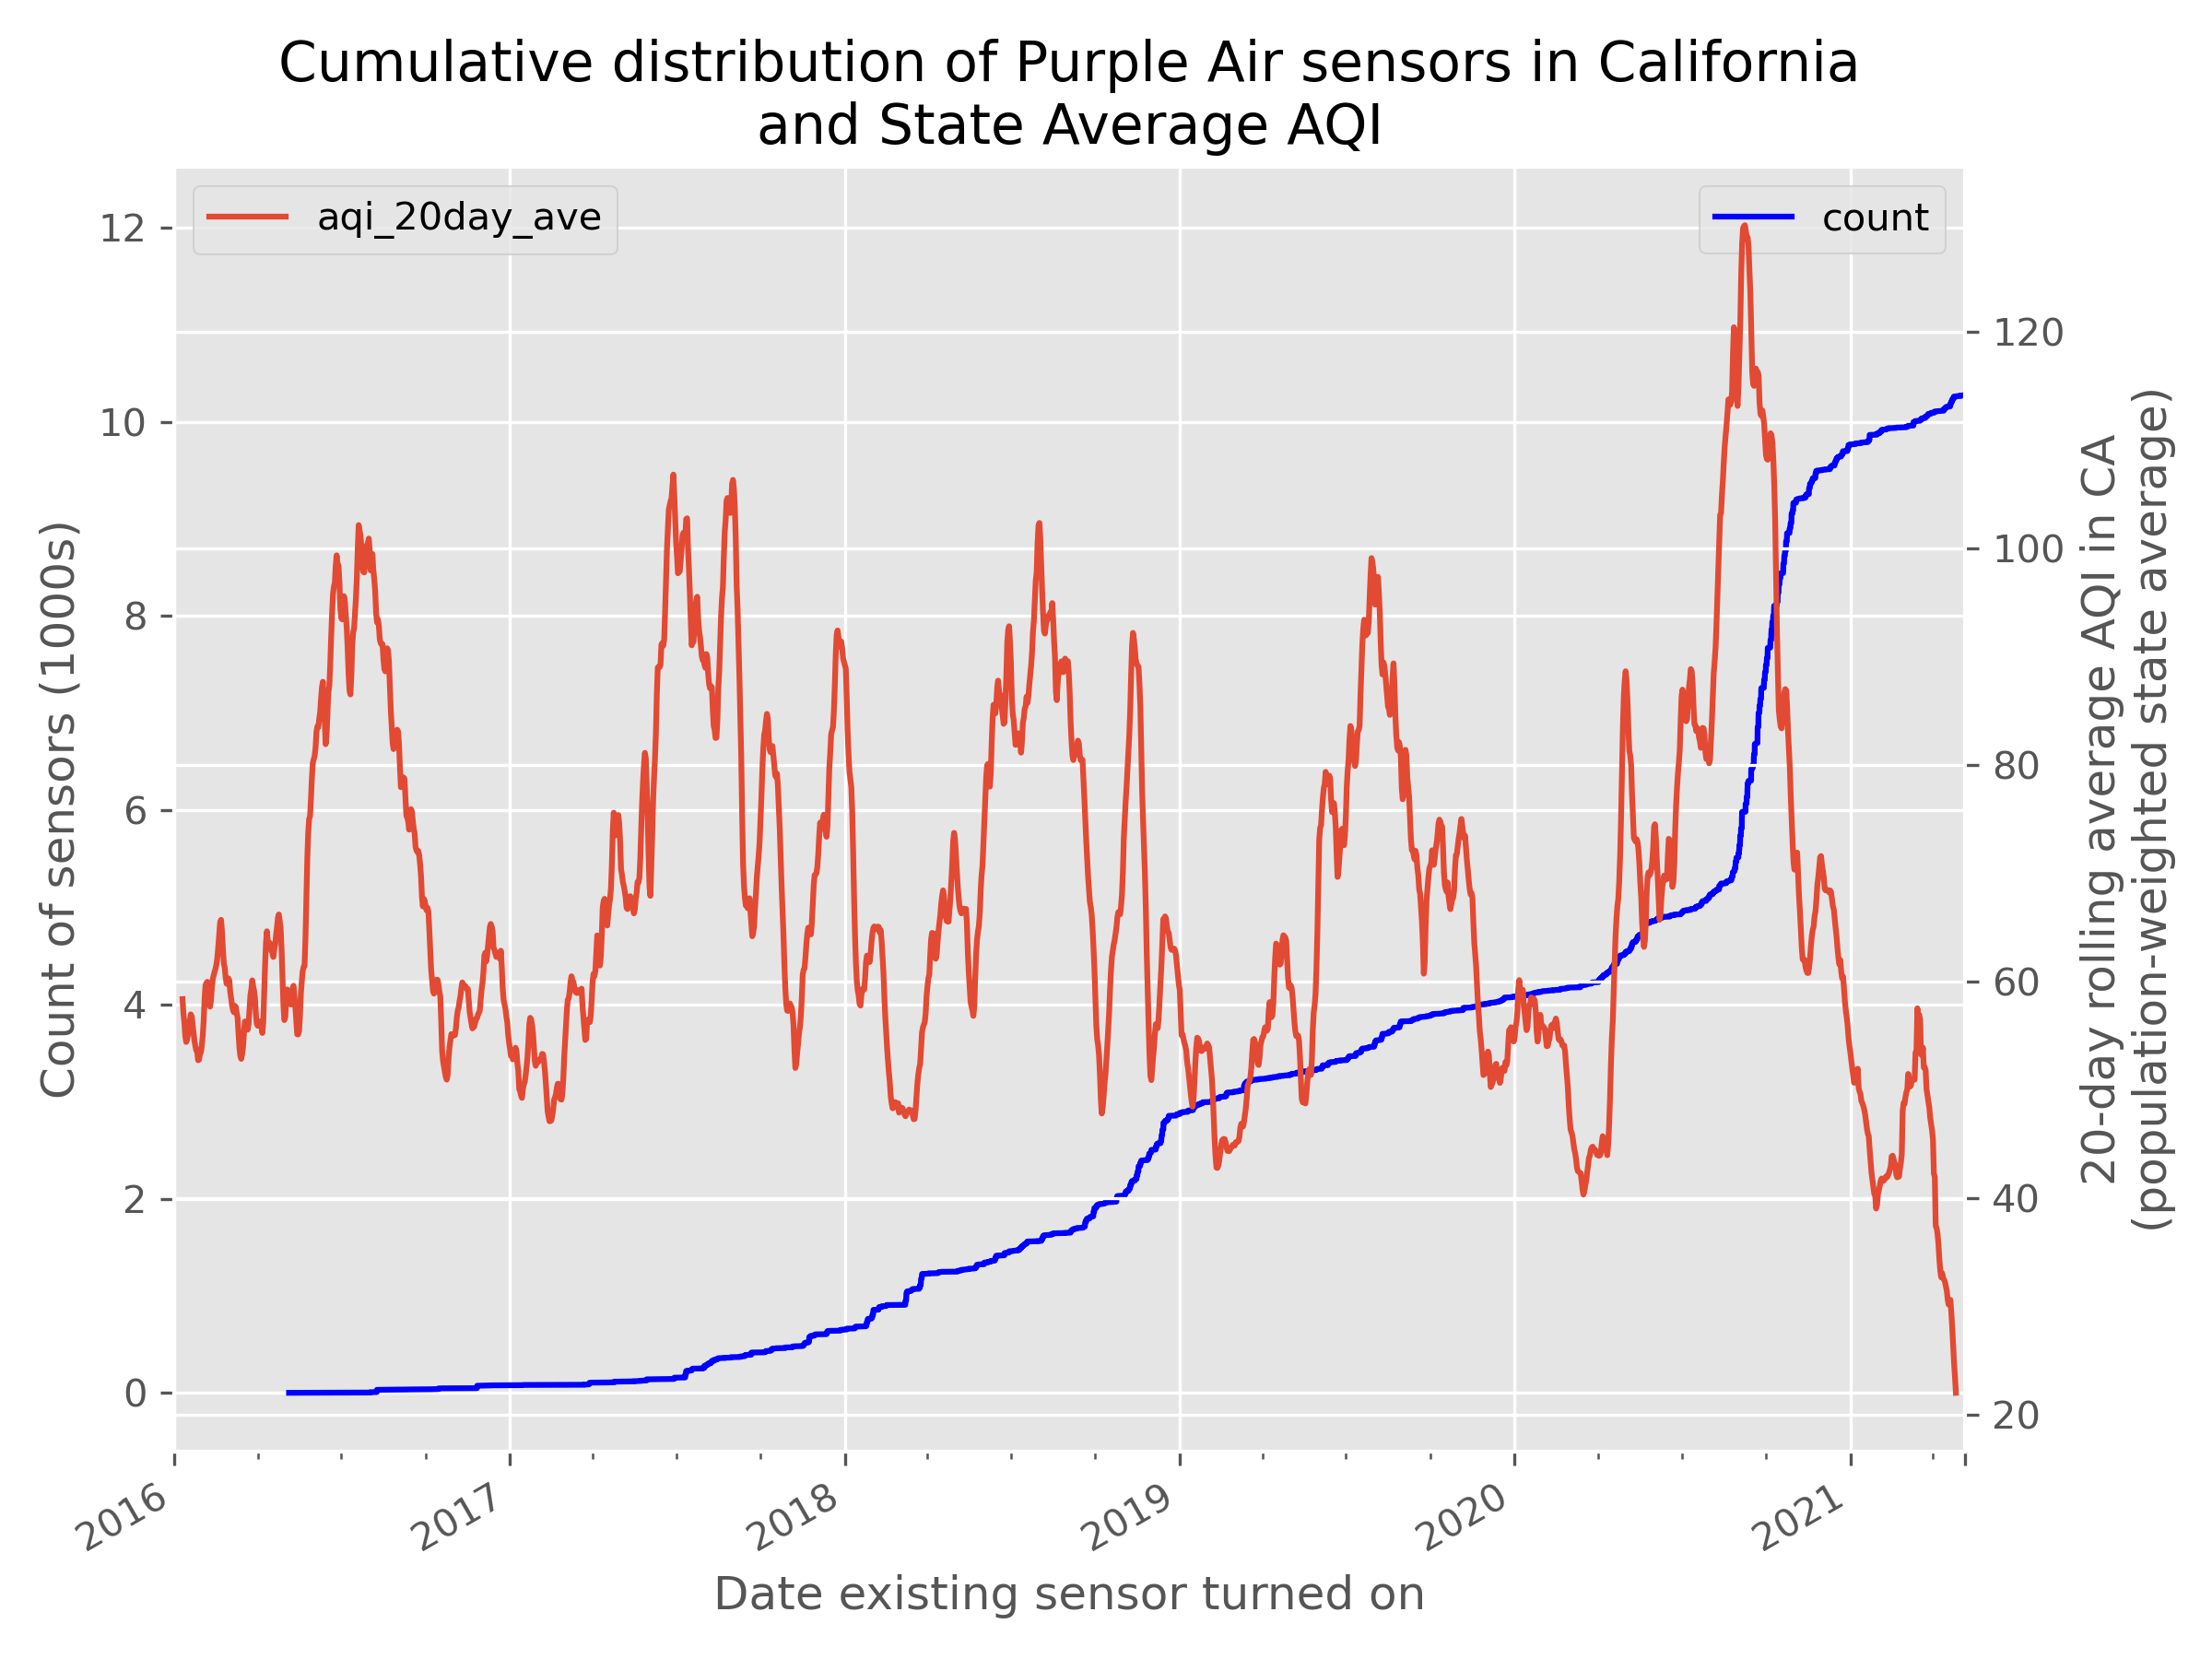
\includegraphics[width=0.8\textwidth]{purple_air_sensor_cum_time_california.png}
% \caption{(Red) 20-day rolling average of the Air Quality Index in California. (Blue) Cumulative PurpleAir outdoor sensors posting public PM2.5 data.}
% \label{fig:ca_purpleair_adoption}
% \end{figure}

\FloatBarrier
\begin{figure}[ht]
\centering
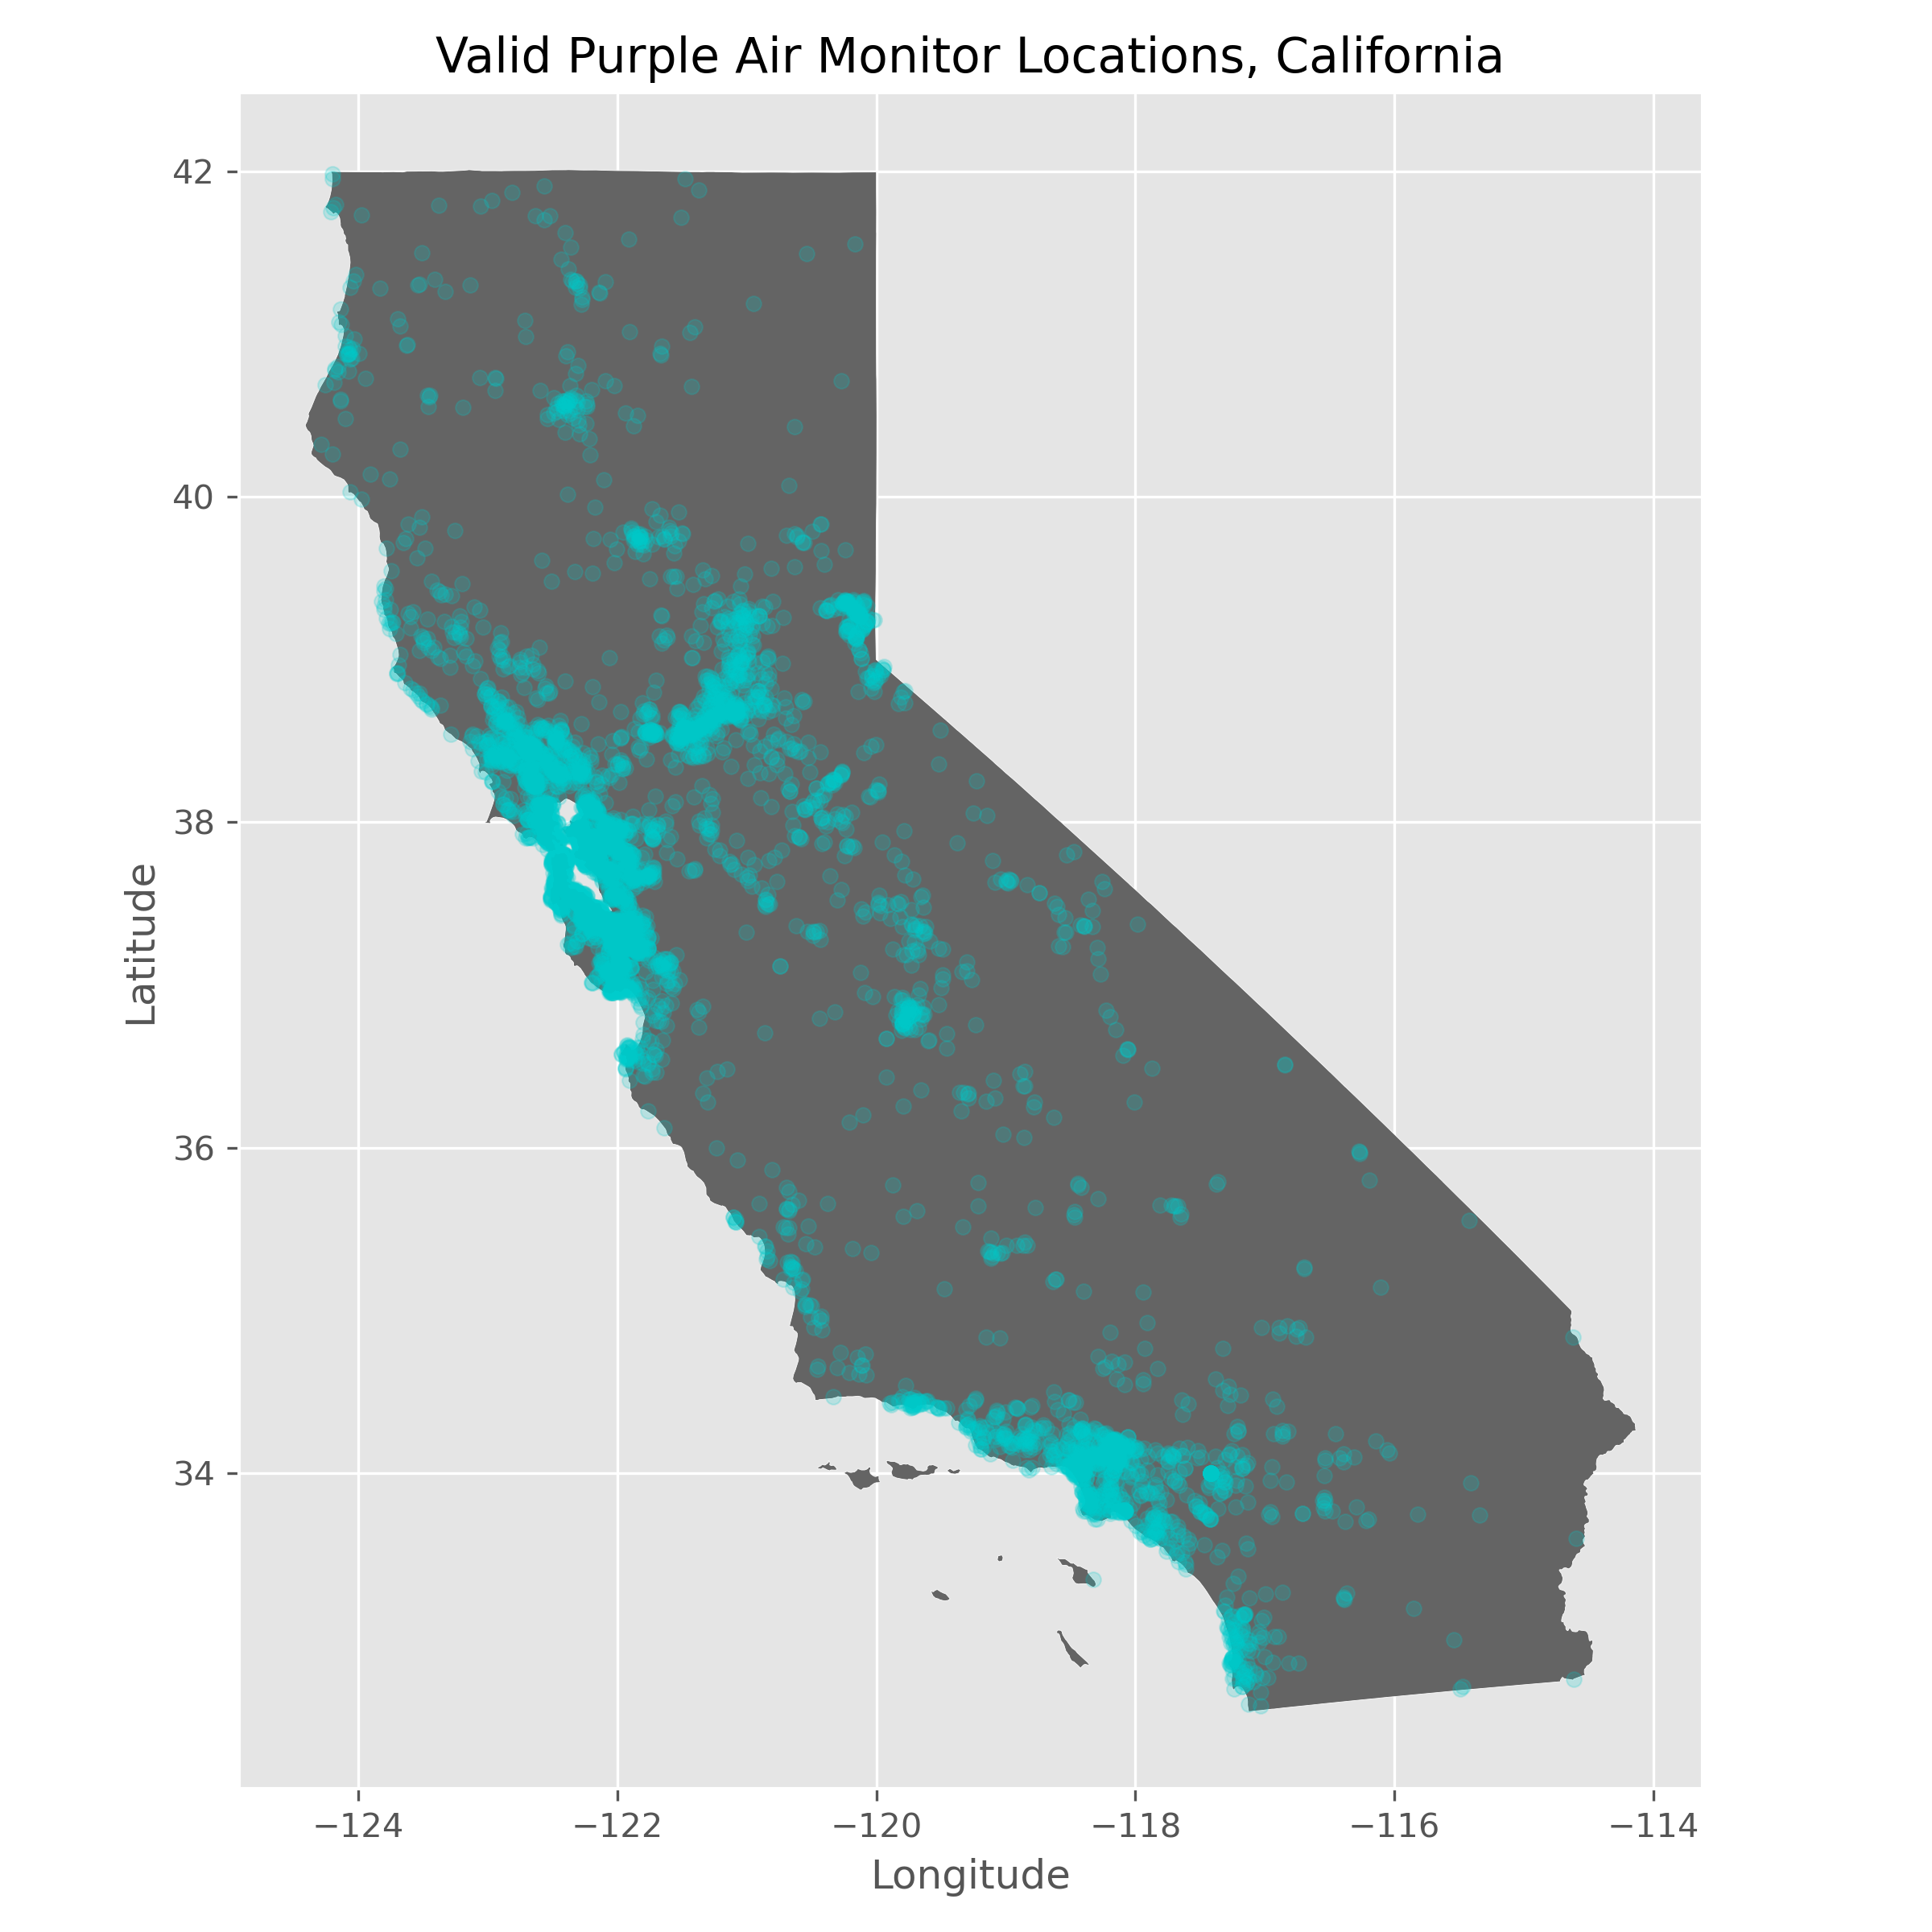
\includegraphics[width=0.8\textwidth]{purple_air_sensor_map_california.png}
\caption{Map of PurpleAir sensors offering public, outdoor PM2.5 measurements. These are sensors that have offered any data in the past, so many are now inactive. The historical data is used in this analysis.}
\label{fig:ca_purpleair_map}
\end{figure}

\FloatBarrier
\textbf{PurpleAir and a NAAQS Monitor.} As an example, figure \ref{fig:concentric_purpleair_037-4004} depicts the high number of PurpleAir sensors in the vacinity of one of Los Angeles's NAAQS monitors. I select the PurpleAir sensors in pink, those within 5 miles of the monitor.
\begin{figure}[ht]
\centering
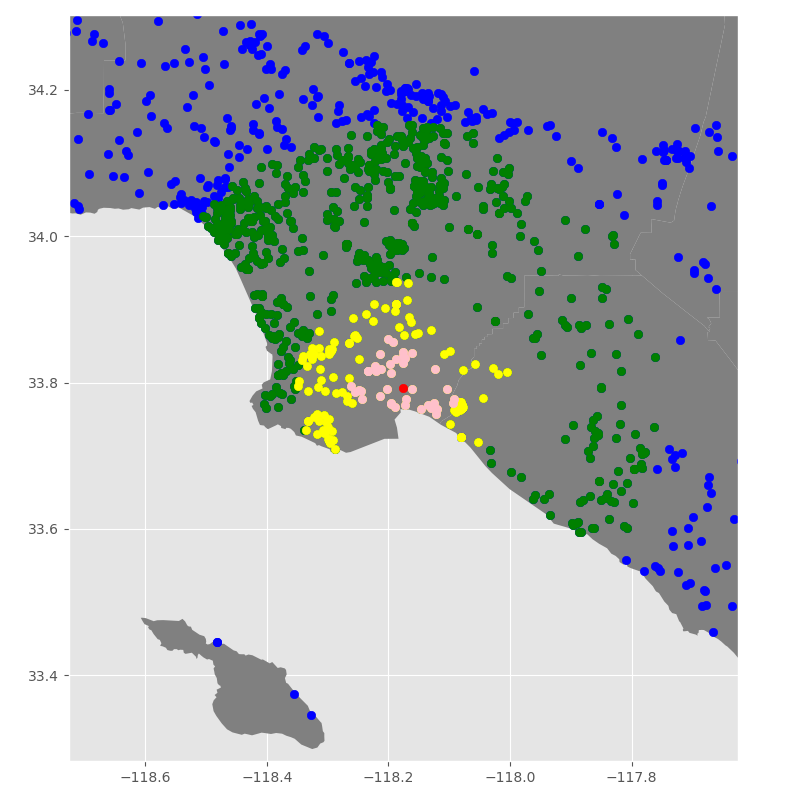
\includegraphics[width=0.8\textwidth]{county-037_site-4004_epa-pa-concentric-ranges.png}
\caption{Map of an EPA NAAQS-primary monitoring station (red) surrounded by PurpleAir monitors within 5-mile (pink), 10-mile (yellow), and 25-mile (green) radii. This preliminary analysis uses the PurpleAir sensors within 5 miles (pink markers).}
\label{fig:concentric_purpleair_037-4004}
\end{figure}

% \FloatBarrier
% \begin{figure}[ht]
% \centering
% 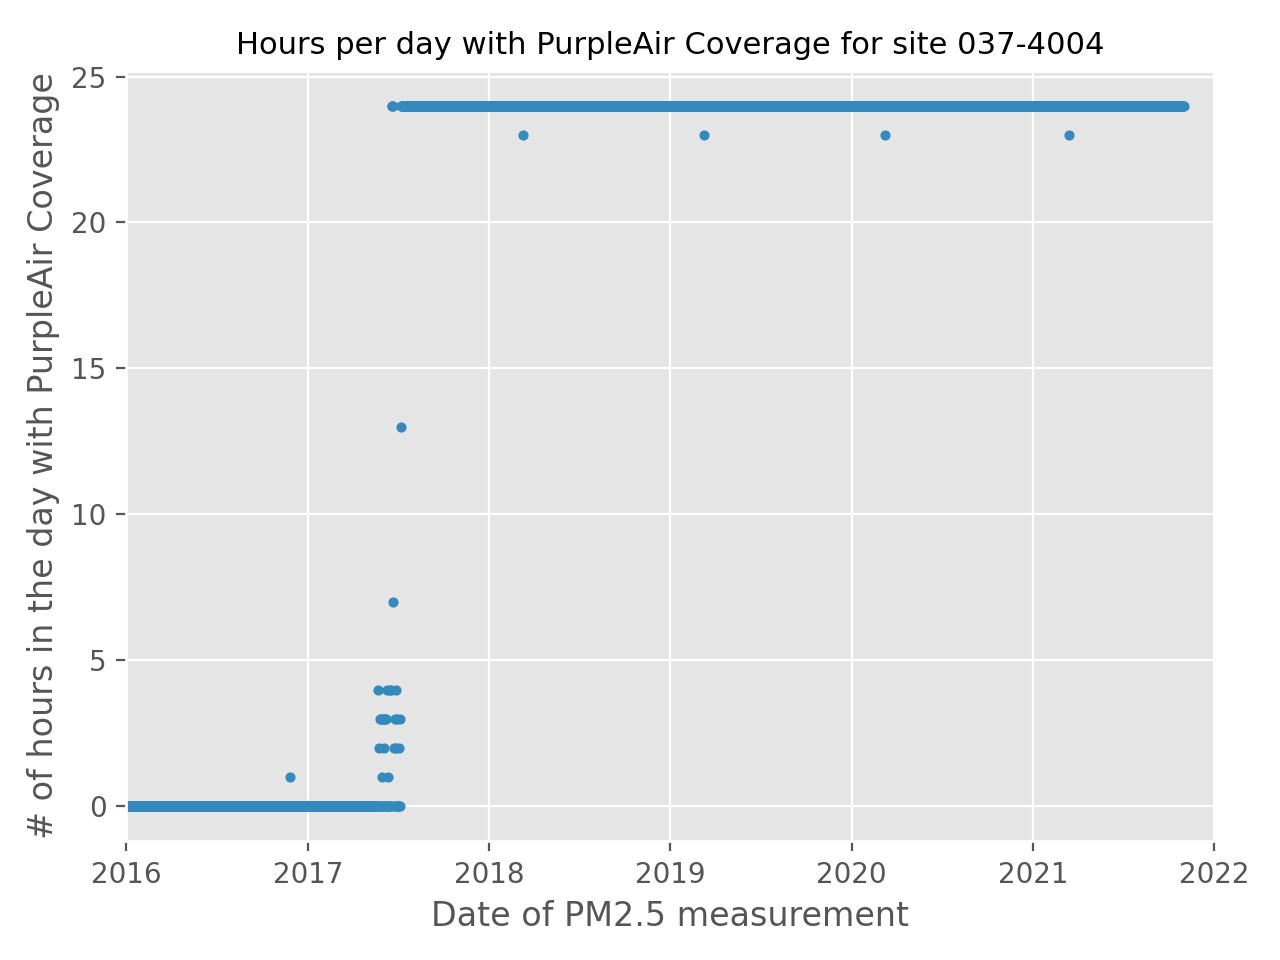
\includegraphics[width=0.8\textwidth]{site-037-4004_pa-daily-covereage.png}
% \caption{Scatter plot indicating the number of hours in each day that this NAAQS-primary monitor has PurpleAir coverage. An hour has PurpleAir coverage if there are any PurpleAir sensor readings within the 5-mile radius of the monitor site for that hour. The weighted average is calculated for that hour using all the available PurpleAir readings within 5 miles.}
% \label{fig:hourly_coverage_037-4004}
% \end{figure}


\FloatBarrier
\begin{figure}[ht]
\centering
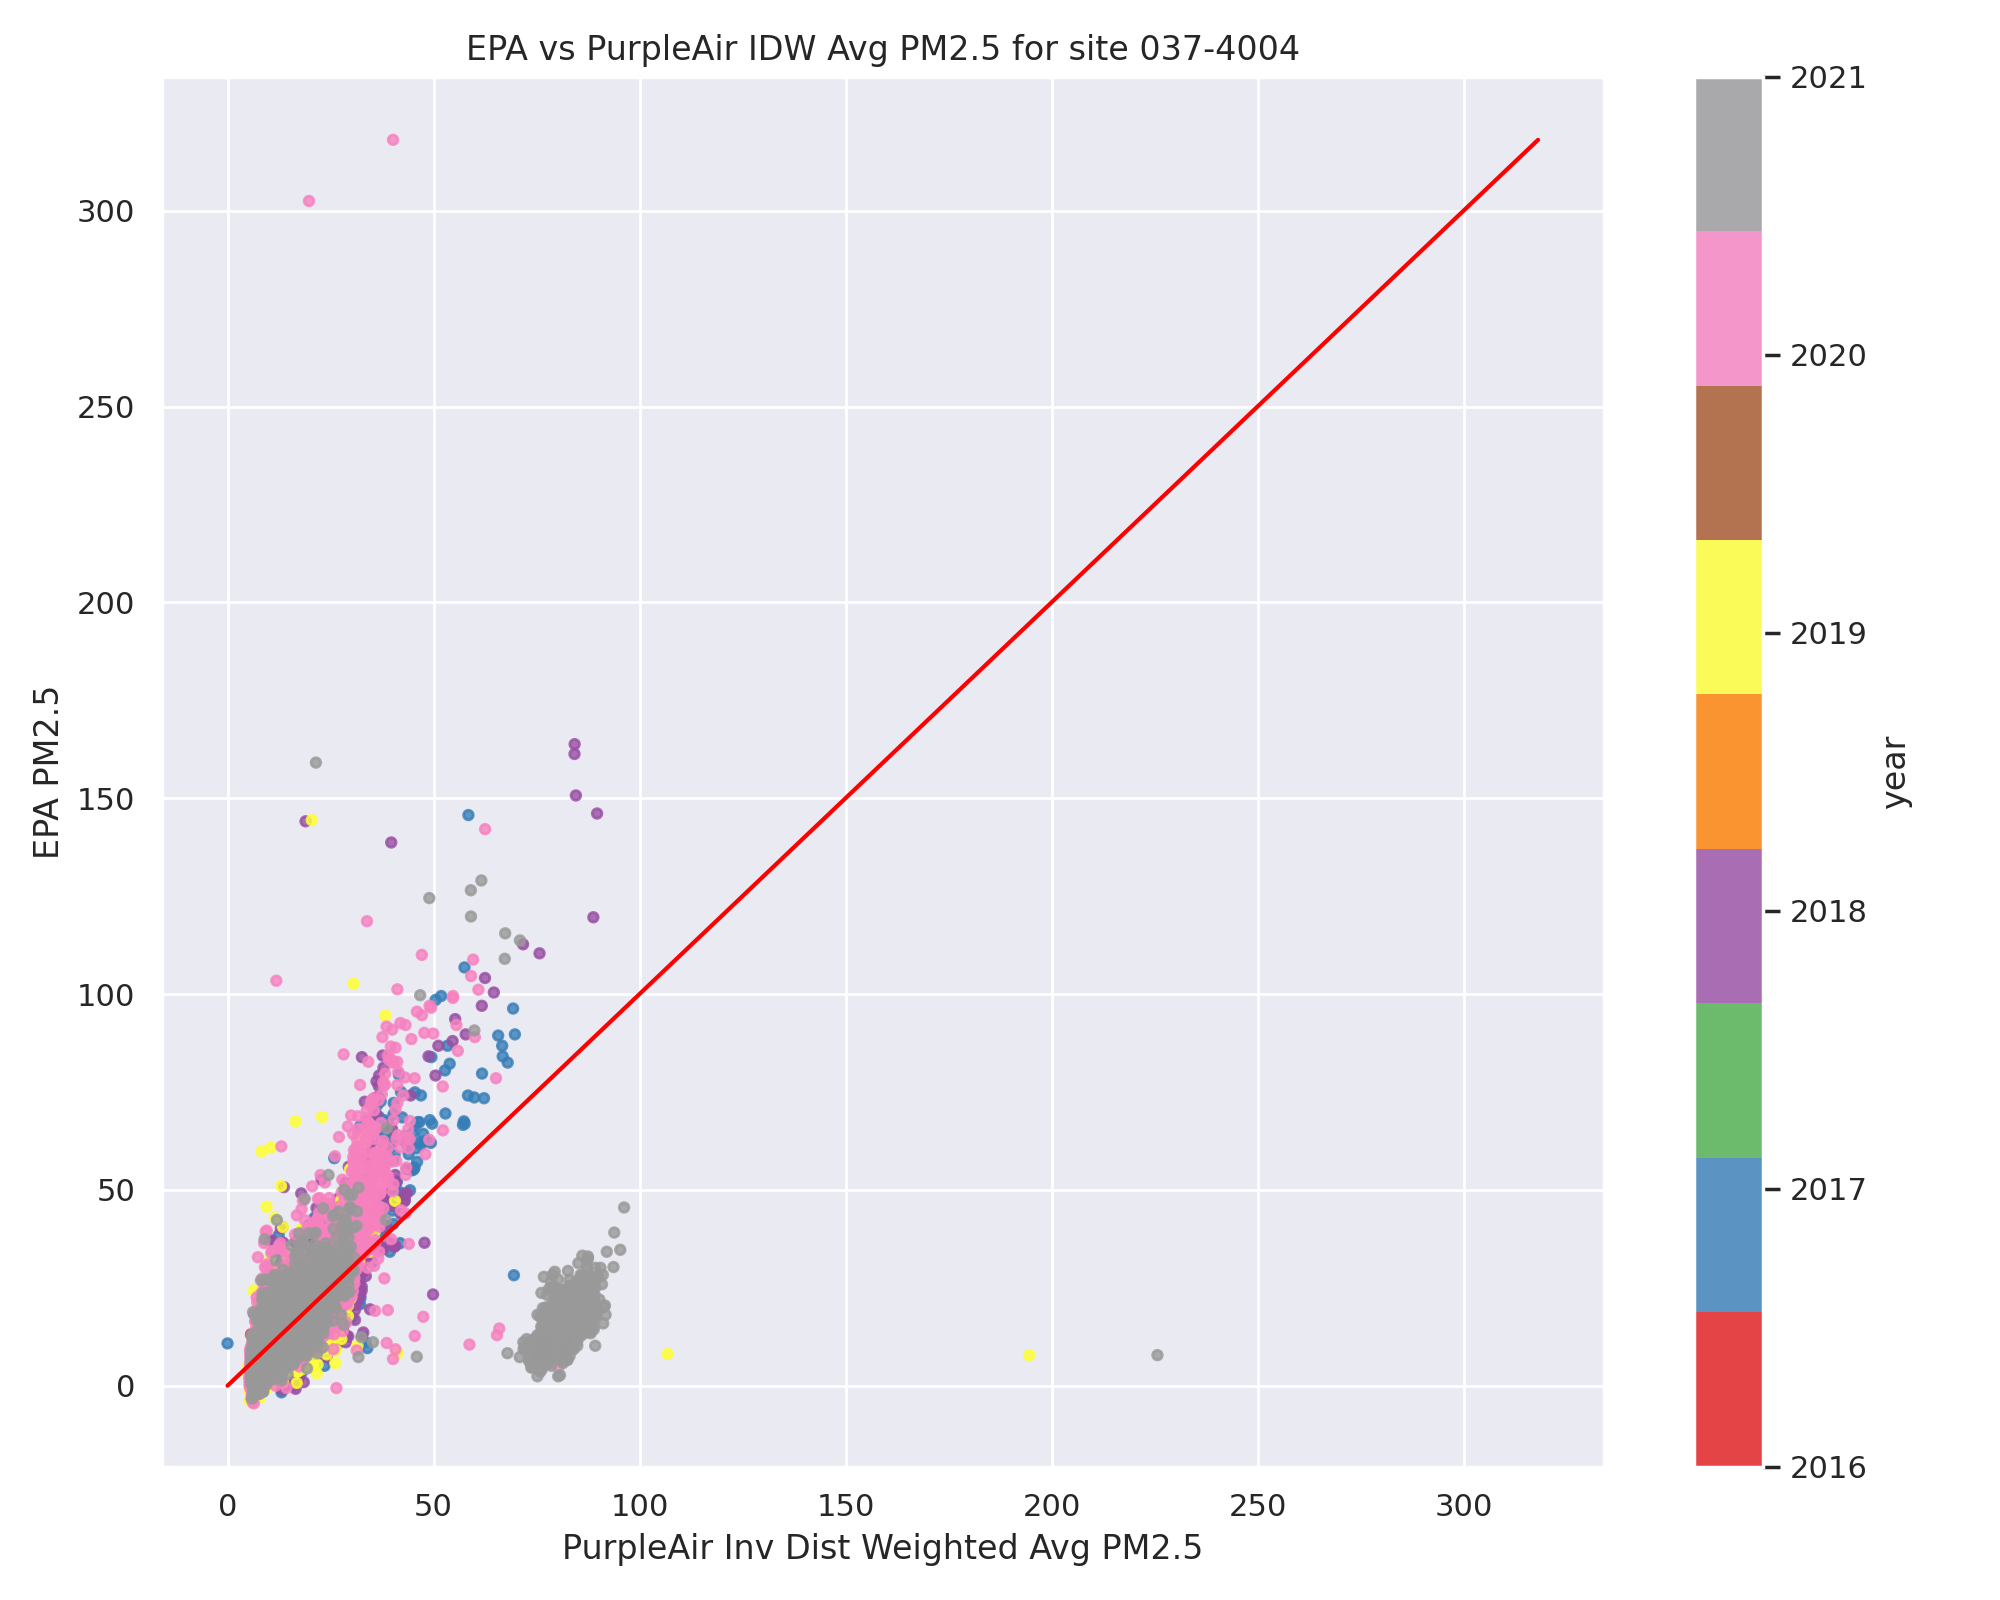
\includegraphics[width=0.8\textwidth]{site-037-4004_epa-pa-hourly-plot.png}
\caption{Scatter plot comparing reported hourly PM2.5 measurements: the x-axis represents the IDW-weighted average of PurpleAir measurements, the y-axis represents reported NAAQS-primary monitor measurements. The red line is a 45$^\circ$ line, representing perfect correlation between the PurpleAir average and the NAAQS-primary monitor. For this site, we can see the PurpleAir average is skewed to the right for readings from 2021. This is likely from a PurpleAir sensor coming online that was placed near a source of localized pollution that is not being picked up by the NAAQS-primary monitor.}
\label{fig:pa-epa-compare_037-4004}
\end{figure}


\FloatBarrier
% \subsection{Wind Speed and Direction}

\subsection{Estimating Regulation-grade Readings with PurpleAir Sensors} 
I use inverse-distance weighting (IDW) with a power of 1 on the denominator. In their discussion of IDW in ambient pollution estimation, \cite{demesnardPollutionModelsInverse2013} derives that a power between 1 and 3 is appropriate for diffuse particle distributions. I use a power of 1 here because I find evidence that some PurpleAir sensors that are very close to the NAAQS monitor are not very good predictors of the monitor's PM2.5 levels. These PurpleAir sensors seem to still have reliable estimates\footnote{Each PurpleAir sensor has two internal sensors that measure PM2.5. Reliability of the PurpleAir sensors is determined by the agreement of the two sensors' hourly averages.}, and anecdotally seem to have very high PM2.5 readings when they disagree with the NAAQS monitor. This suggests they are measuring localized pollution that is out of the range of the NAAQS monitor (these sensors could be located next to a highway, for example).

I plan to fix this issue with a future implementation of a better prediction model\footnote{See Appendix section \ref{sec:app-prediction}}. In this iteration, I have implemented the sub-optimal IDW average to avoid excluding entire PurpleAir sensors and removing potentially useful sensor data.









%===========================================
\section{Theoretical \& Empirical Framework} 
\label{theoretical}
%===========================================

\subsection{Estimating PM2.5 at the NAAQS Monitor with PurpleAir Sensors}
\FloatBarrier

To examine the difference between reported pollution and that which is missing from the NAAQS monitors' dataset, I need some measure of ambient PM2.5 levels around the monitor. A good place to start is inverse distance weighting (IDW) to create a weighted average of PurpleAir sensors that can tell us about the PM2.5 levels near the NAAQS monitor.\footnote{This is not a good place to end, however. IDW produces fairly poor estimates of PM2.5 at the location of the NAAQS monitor (before OLS). I plan to implement a more rich prediction model using wind speed and direction -- see the Appendix section \ref{sec:app-prediction} for model and data notes on this method. Ultimately, both satellite and PurpleAir data could be combined with NAAQS monitor data to provide a more accurate depiction of pollution in the US.} To help make the estimation process concrete, I will use a monitor in Los Angeles, CA as an example (see Fig. \ref{fig:idw_diagram} for a visual representation).

\begin{figure}
  \begin{center}
    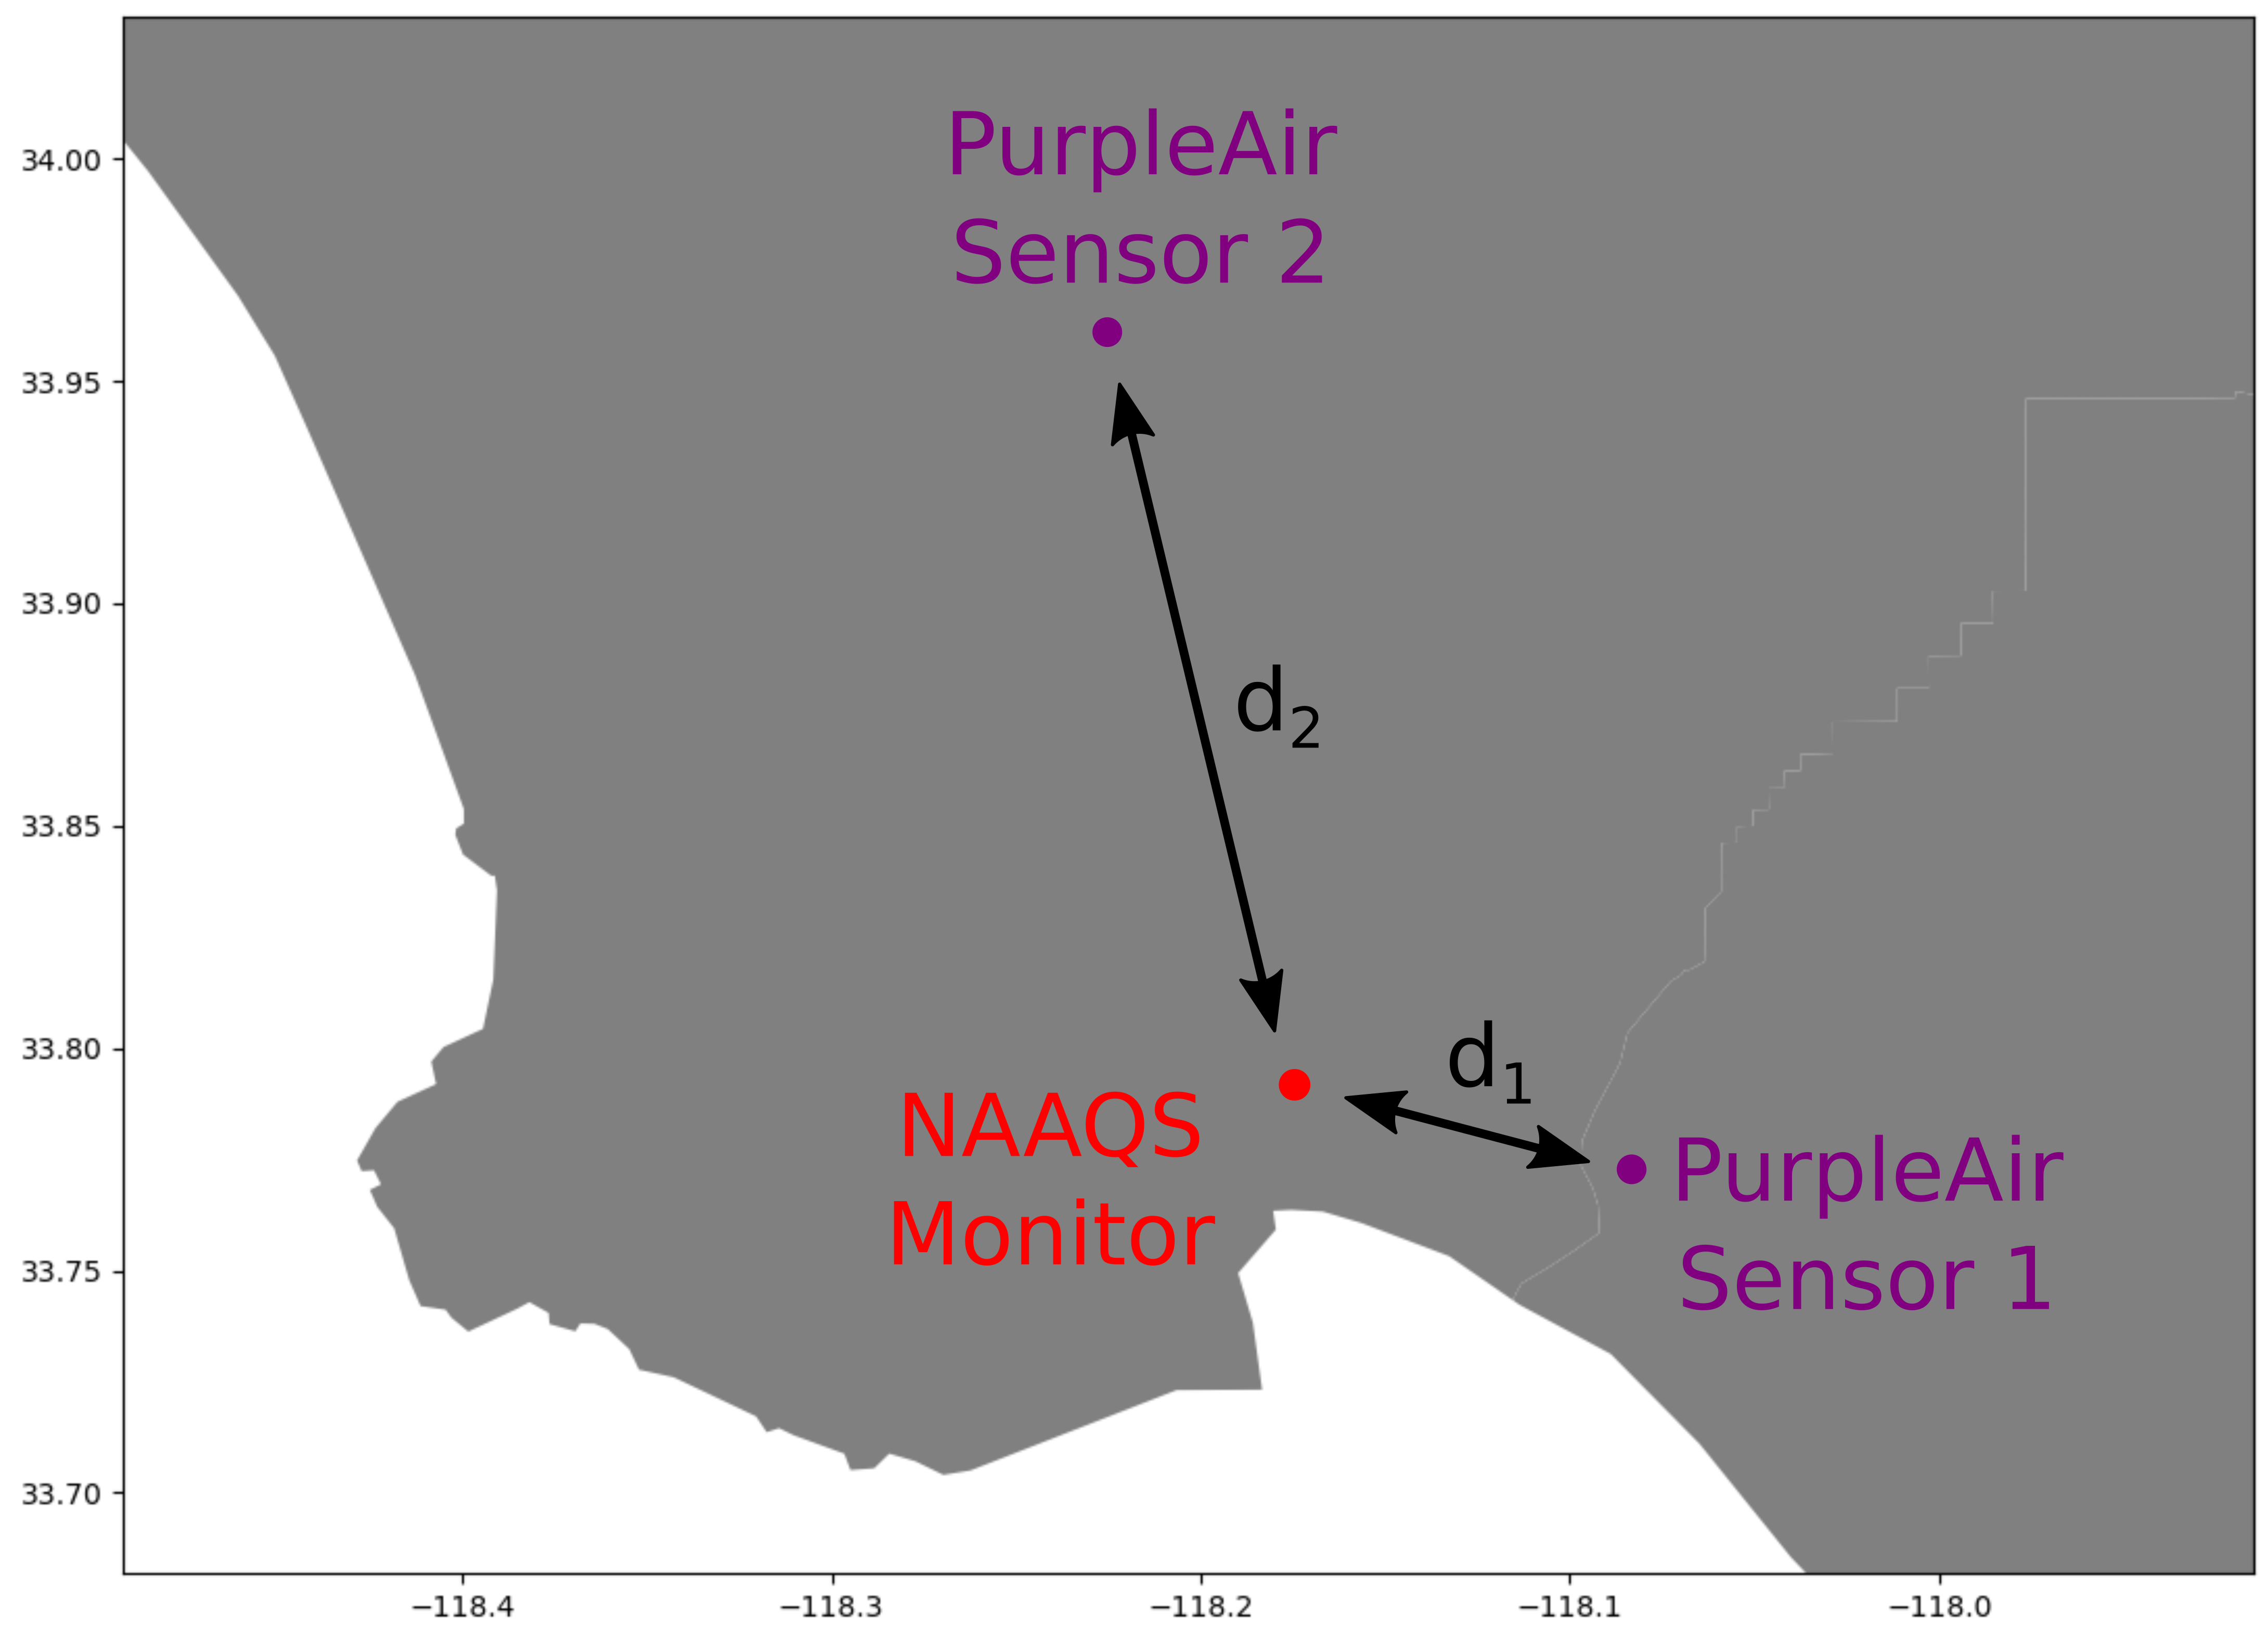
\includegraphics[width=0.48\textwidth]{IDW_diagram}
  \end{center}
  \caption{Example distances of two selected PurpleAir sensors near a NAAQS monitor in Los Angeles, CA.}
  \label{fig:idw_diagram}
\end{figure}

Consider an EPA NAAQS monitor that measures PM2.5 concentration $EPA_T$ at time $t$. Let $PA_{j,t}$ be PM2.5 concentration as measured by PurpleAir sensor $j$ at time $t$ at a distance $d_j$ from the NAAQS monitor. Assume that there are $J_t$ active PurpleAir sensors in the vicinity of the NAAQS monitor at some time $t$, each with their own PM measurements and distance. Then the Inverse-Distance Weighted average PurpleAir PM reading $PA^{IDW}_{j,t}$ is
\begin{equation}
    PA^{IDW}_t= \sum\limits_{j=1}^{J_t} \dfrac{\frac{1}{d_j}\cdot PA_{j,t}}{\sum\limits_j^{J_t}\frac{1}{d_j}}
    = \sum\limits_{j=1}^{J^t} w_{j,t}\cdot PA_{j,t}
\end{equation}
Note here that I am explicitly using the exponent of one on the distance to balance the desire to have closer sensors provide more weight but avoid having extraordinarily large weights on sensors that are relatively close to the monitor. Also note that the number of PurpleAir sensors $J_t$ changes over time as sensors come online and exit. This means the weights of the weighted average need to be calculated separately for each period. This IDW average PurpleAir measurement provides me with a measure of ambient PM2.5 variation in the vicinity of the NAAQS monitor at all the possible times there exists at least one PurpleAir monitor in the area. This helps provide good coverage and make implementing OLS in the next step easier. 

\textbf{OLS Prediction.} Even if the PurpleAir sensors are highly accurate at measuring PM2.5 concentrations at their location, they may still biased as measures of PM2.5 near the NAAQS monitor. For example, someone might put up a PurpleAir sensor on a telephone pole right next to a highway, which might have high average PM compared to where the NAAQS monitor is placed. To help ensure an unbiased approximation of the missing monitor measurements \textit{at the location of the NAAQS monitor}, I use OLS to regress the NAAQS monitor data on the weighted average PurpleAir data.

\begin{equation}
EPA_t = \beta_0 + \beta_1 PA^{IDW}_t + \varepsilon_t
\end{equation}

\def\M{\mathcal{M}}\def\N{\mathcal{N}}\def\R{\mathbbm{R}}
\def\up{\widehat{EPA}^U_t} \def\low{\widehat{EPA}^L_t}
I then predict missing NAAQS monitor data (out of sample) and combine the predicted PM estimate with the reported readings. Formally, suppose $\M$ is the set of \textbf{missing} times that we do not have a PM record from the NAAQS monitor (i.e., $EPA_t$ does not exist for $t\in\M$). Let $\N$ be the \textbf{non-missing} (reported) times for the NAAQS monitor ($EPA_t\in\R\ \forall t\in\N$). For simplicity, assume that some PurpleAir data are available at all times ($PA^{IDW}_t\in\R_+\ \forall t\in\M\bigcup\N$). Using the PurpleAir data during the missing times, I predict the missing NAAQS data:

\begin{equation}
\widehat{EPA}_t = \hat\beta_0 + \hat\beta_1 PA^{IDW}_t \quad \forall t\in\M
\end{equation}

I also estimate the 95\% lower and upper bound on each predicted value; $\low$ and $\up$ to later using in lower and upper bounds on the design value.

\subsection{Estimating Design Values} \label{design_value_equations}
The NAAQS specify two primary statistics to determine if an area is in or out of attainment. These two statistics are referred to as the Annual and 24-hour Design Values. The annual design value is a 3-year average of annual averages of daily average PM2.5 levels. The 24-hour design value is a 3-year average of the annual 98th percentile of daily averages. There are also considerations about the proportion of allowed missing recordings (75\%). See Appendix Section \ref{sec:design_values} for details on constructing these design values.

\def\dva{\text{DV}_A}\def\dvh{\text{DV}_H}
\def\dvaa{\widetilde{\text{DV}}_A}\def\dvhh{\widetilde{\text{DV}_H}}
I first construct design values using the reported NAAQS monitor data. In the style of \cite{fowlieBringingSatelliteBasedAir2019}, I will call these annual and 24-hour \textit{pseudo design values}; $\dva$ and $\dvh$. I do not use the reported design values because there is a more complex negotiation that happens between the EPA and state regulators that can change some of the numbers. In order to compare design values between reported and reported + imputed datasets, I must calculate them on the actual reported PM2.5 readings from the NAAQS monitor.

I then create predicted NAAQS PM values using PurpleAir data as described in the previous section. I replace all missing NAAQS monitor values possible with the predicted values, leaving the original valid NAAQS readings. With this new imputed dataset, I calculate the new imputed design values: $\dvaa$ and $\dvhh$. Subtracting the original design value from the imputed design value gives an estimate of design value bias caused by missing data.

\begin{align}
    \text{bias}^{miss}(\dva) &\approx \dvaa - \dva\\
    \text{bias}^{miss}(\dvh) &\approx \dvhh - \dvh
\end{align}

If this quantity is positive, then there is support that there is under-reporting of pollution via allowed missing data. To gain an understanding of significance of the results, I also propagate the upper and lower bounds of the predicted observations through the design value calculation (similar to \cite{fowlieBringingSatelliteBasedAir2019}, but they were estimating out of sample prediction errors). This provides a 95\% confidence interval -- upper and lower bounds on the imputed design values: $\dvaa^{upper}$,  $\dvaa^{lower}$, $\dvhh^{upper}$, and $\dvhh^{lower}$.

\textbf{NAAQS.} The standards set out in the National Ambient Air Quality Standards give specific thresholds to compare the design values to. Above the thresholds are considered nonattainment. The primary standard for the annual design value is 12 $\mu$g/m$^3$, and has a secondary standard of 12 $\mu$g/m$^3$. The 24-hour standard is 35 $\mu$g/m$^3$.


\textbf{Exceptional Events.} As mentioned in section 3, there are many events for which the EPA allows local regulators to exclude their readings from design value calculations. These readings were removed from the dataset before any design value calculations and do not get imputed.









%==============================================
\section{Results and Discussion}
\label{results}
%==============================================
I conducted 15 design value tests on 15 different NAAQS monitors. To create the predicted design value for each NAAQS monitor, I regressed the NAAQS monitor PM2.5 readings on the weighted average PurpleAir readings. An example of this regression is below for one of the Los Angeles monitors. I ran regions both with an without a constant, but because I wanted the prediction errors to have mean zero, I chose to use model (2) in the creation of the design value. Note that the $R^2$ value in model (1) is much higher, however $R^2$ values between regressions with constant and those without are no comparable due to the difference in denominators. 
\begin{table}[!htbp] \centering
  \caption{037-4004 NAAQS Monitor PM2.5 on Weighted Average PurpleAir PM2.5}
  \label{tab:reg_037-4004}
\begin{tabular}{@{\extracolsep{5pt}}lcc}
\\[-1.8ex]\hline
\hline \\[-1.8ex]
& \multicolumn{2}{c}{\textit{Reported NAAQS Monitor PM2.5}} \
\cr \cline{2-3}
\\[-1.8ex] & (1) & (2) \\
\hline \\[-1.8ex]
 const & & 6.924$^{***}$ \\
  & & (0.076) \\
 PurpleAir IDW Average & 0.741$^{***}$ & 0.444$^{***}$ \\
  & (0.003) & (0.004) \\
\hline \\[-1.8ex]
 Preferred & No & Yes \\
 Observations & 36,813 & 36,813 \\
 $R^2$ & 0.658 & 0.240 \\
 Adjusted $R^2$ & 0.658 & 0.240 \\
 Residual Std. Error & 9.870 & 8.920  \\
 F Statistic & 70924.412$^{***}$  & 11642.169$^{***}$  \\
\hline
\hline \\[-1.8ex]
\textit{Note:} & \multicolumn{2}{r}{$^{*}$p$<$0.1; $^{**}$p$<$0.05; $^{***}$p$<$0.01} \\
\end{tabular}
\end{table}

The number of observations here are the number of hours between 2016 and 2021 where neither the NAAQS monitor or the weighted average PurpleAir readings were missing. The slope in both models is less than one, indicating that PurpleAir tends to measure higher PM2.5 concentrations. This could be a selection issue -- consumers who choose to buy a PurpleAir monitor and place it outside their house are probably concerned about pollution -- or a measurement difference between the types of devices.

 For all sites, I generated kernel density plots like those in Fig. \ref{fig:missing-density_019-0500}. Only one of the 15 sites I tested had noticeable differences in the PM2.5 distributions for missing and reported hours (see the appendix for all sites' plots). However, the design values are the policy-relevant statistic of those distributions. Looking at the top and bottom figures below however, we can guess that the means and 98th percentile might be similar in the top case, and could plausibly be different in the bottom case.

 
\begin{figure}
\centering
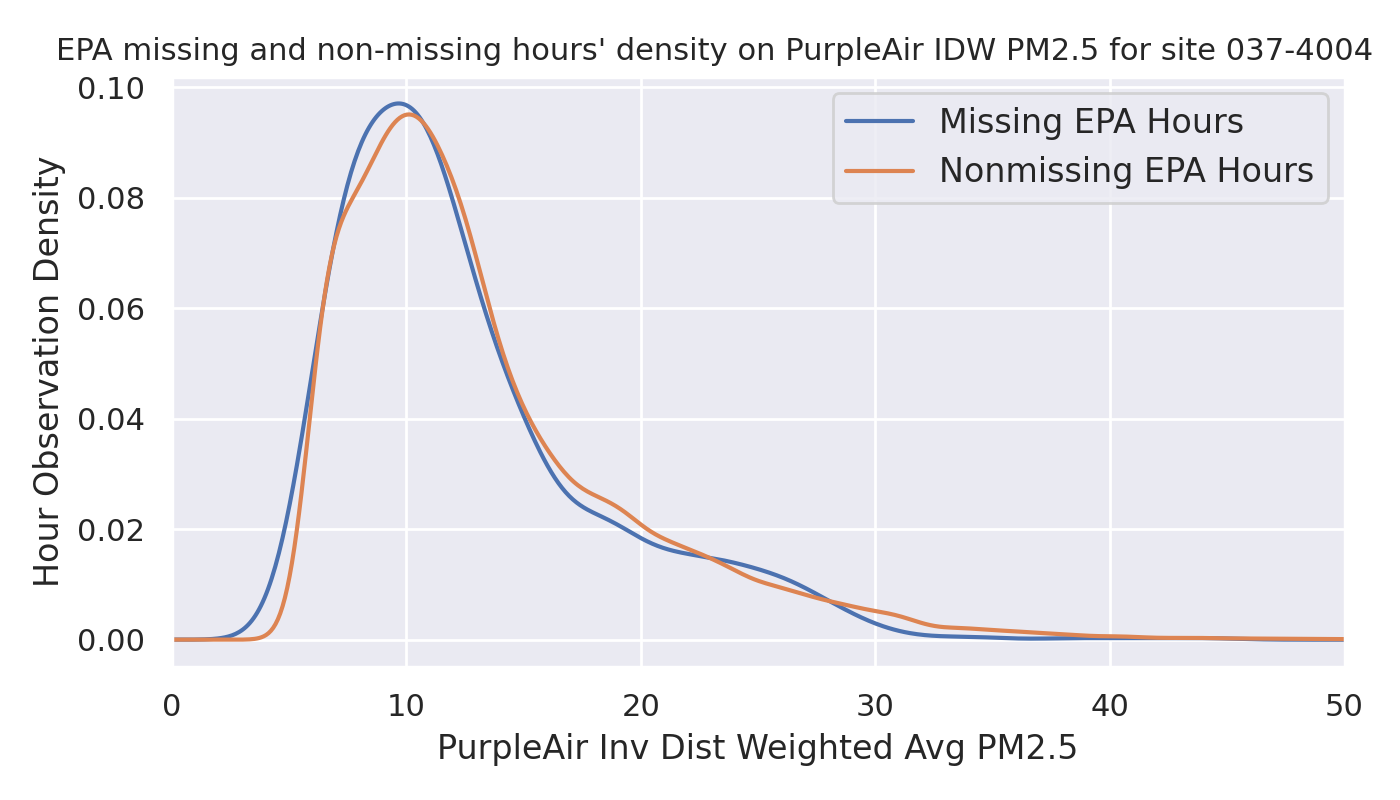
\includegraphics[width=0.6\textwidth]{site-037-4004_epa-pa-missing-density.png}
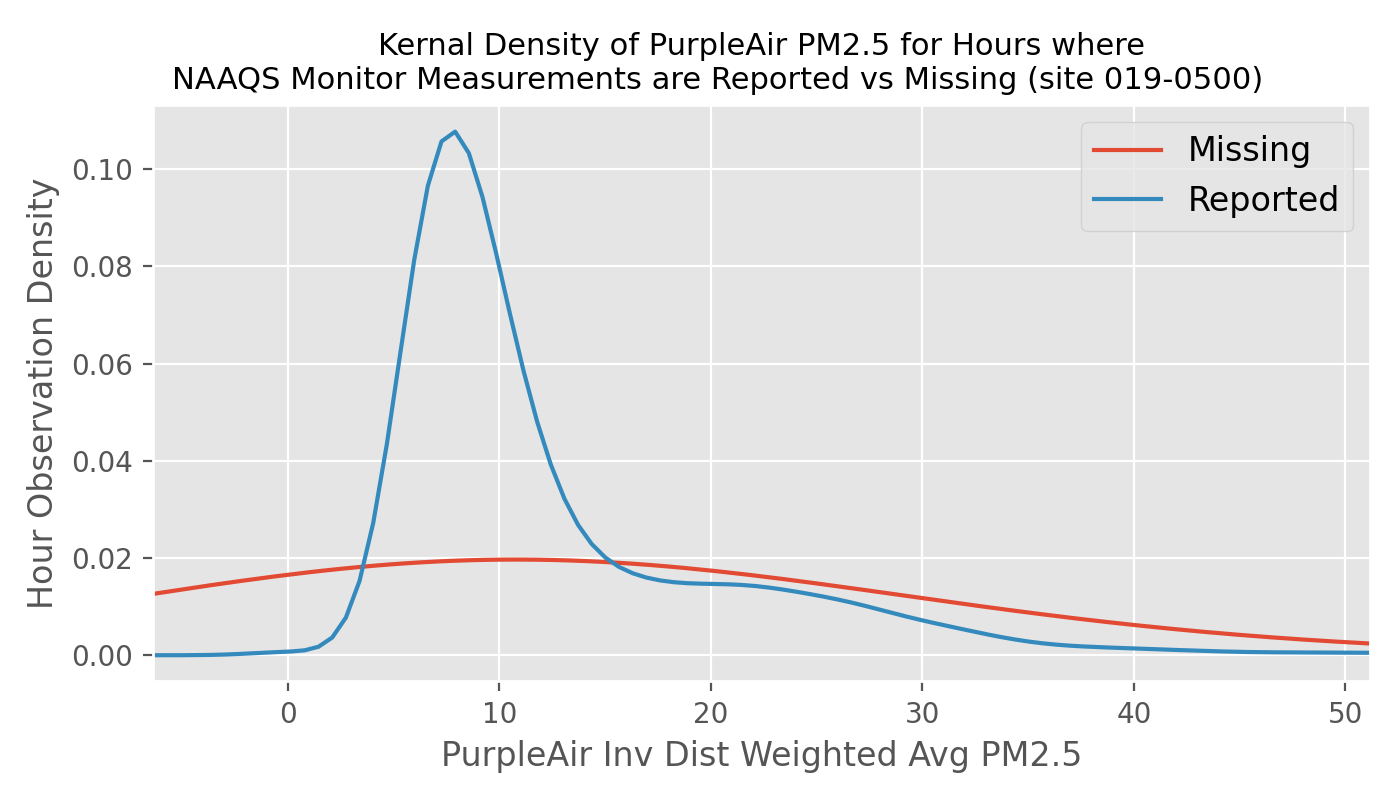
\includegraphics[width=0.6\textwidth]{appendix/site_plots/site-019-0500_epa-pa-missing-density.png}
\caption{Comparison of estimated kernel densities of PM2.5 concentration for two sets of hours: reported (blue) and missing (red) hourly observations of the NAAQS monitor. Both densities use the hourly PurpleAir PM2.5 concentration estimates for this site, calculated using the IDW average of PurpleAir sensors within 5 miles of the NAAQS monitor location. The top image is for a monitor at a site in LA, and the bottom is at a site in Fresno, CA.}
\label{fig:missing-density_019-0500}
\end{figure}





\begin{table}[]
\caption{Design Value Comparison for Fresno, CA. (98\% CI Bounds)}
\label{tab:fresno_dvs}
\resizebox{\textwidth}{!}{%
\begin{tabular}{@{}l|lll|lll@{}}
Year-Quarter & \begin{tabular}[c]{@{}l@{}}Annual DV\\ Difference\end{tabular} & \begin{tabular}[c]{@{}l@{}}Upper \\ Bound\end{tabular} & \begin{tabular}[c]{@{}l@{}}Lower\\ Bound\end{tabular} & \begin{tabular}[c]{@{}l@{}}Hour DV \\ Difference\end{tabular} & \begin{tabular}[c]{@{}l@{}}Upper \\ Bound\end{tabular} & \begin{tabular}[c]{@{}l@{}}Lower \\ Bound\end{tabular} \\ \midrule
2018-4 & Invalid DV &  &  & Invalid DV &  &  \\
2019-1 & -0.005 & 0.133 & -0.143 & 0.000 & 0.252 & 0.000 \\
2019-2 & -0.003 & 0.141 & -0.147 & 0.000 & 0.252 & 0.000 \\
2019-3 & 0.015 & 0.170 & -0.139 & 0.058 & 2.202 & 0.000 \\
2019-4 & 0.002 & 0.190 & -0.185 & 0.000 & 1.460 & -0.024 \\
2020-1 & -0.012 & 0.182 & -0.207 & 0.000 & 0.335 & 0.000 \\
2020-2 & -0.010 & 0.191 & -0.211 & 0.000 & 0.376 & 0.000 \\
2020-3 & 0.679 & 0.954 & 0.403 & 8.718 & 11.704 & 8.556 \\
2020-4 & 0.647 & 1.006 & 0.288 & 5.979 & 8.281 & 5.851 \\
2021-1 & 0.564 & 1.036 & 0.091 & 3.007 & 4.184 & 2.903 \\
2021-2 & 0.533 & 1.024 & 0.042 & 3.007 & 4.225 & 2.903 \\
2021-3 & 0.630 & 1.129 & 0.132 & 7.607 & 10.557 & 7.444
\end{tabular}%
}
\end{table}

Table \ref{tab:fresno_dvs} reports the difference between the pseudo design value (calculated using the reported data) and the imputed design value -- what I believe is an estimate on the design value bias due to low reporting standards. We can see the first row is invalid. This is common in the full results in the Appendix. This occurs because one of the design values have too many invalid days in the quarter (or the 11 quarters before it) the completeness criteria are violated. Examining the Annual design value difference column, the numbers do not seem striking though the lower half do seem to be statistically significant. However, these are not materially significant -- the EPA has rounding conventions (to the ones place) that would make zero effectively within the lower bound since a design value falling below 0.5 would be rounded to 0.

These unremarkable results for the annual design value bias are fairly representative of the batch of 15 sites. When we look at the hour design value results, we can see in 2020 and 2021, there were fairly large and significant differences between the design values. This indicates that having more restrictive data collection standards could have increased Fresno's design value significantly in these quarters. Because OLS was used to impute the missing values, we would expect the hourly imputed values to be unbiased on average. Since we are taking 3-year averages, it seems plausible to believe most bias in the imputation method would average out. These combined with the lower bounds being well above zero suggest there was indeed under-reporting of pollution in Fresno. I cannot say whether or not that it happened intentionally or by mere chance of turning off the monitor at times that would likely have recorded higher pollution.

Is this meaningful for Fresno though? Fresno has had a nonattainment status for many years and is listed on several lists within this literature as having notable pollution measurement issues. So though Fresno's recorded design value would have been higher, they were already well over the 24-hour design threshold of 35 $\mu$g/m$^3$, having pseudo design values in the 50s and 60s in 2020 and 2021.

This is also just one of 15 cases, where the other 14 did not show interesting results. So is this just p-hacking to find the case study that is, by chance, abnormal? In regulation of air pollution, one might be concerned with individual actors or regions trying to get around the regulations. Since the Clean Air Act and the NAAQS are designed to ensure that all American residents can share in a minimum standard, it seems relevant to me to be able to diagnose mismeasurement.

This work is (hopefully) just the beginning of a line of research regarding the distribution of pollution and pollution policies in the US. There is a to-do list in the Appendix.











\newpage
\bibliographystyle{chicago}
\bibliography{references}
% Citation command	Output
% \citet{goossens93}      Goossens et al. (1993)
% \citep{goossens93}      (Goossens et al., 1993)	
% 
% \citet*{goossens93}     Goossens, Mittlebach, and Samarin (1993)
% \citep*{goossens93}     (Goossens, Mittlebach, and Samarin, 1993)
%
% \citeauthor{goossens93}    Goossens et al.
% \citeauthor*{goossens93}   Goossens, Mittlebach, and Samarin

% \citeyear{goossens93}      1993
% \citeyearpar{goossens93}  (1993)

% \citealt{goossens93}     Goossens et al. 1993
% \citealp{goossens93}     Goossens et al., 1993
% \citetext{priv.\ comm.}	(priv. comm.)

\newpage
\section{Appendix}

\subsection{Research Project To-do's} \label{sec:todo}

\textbf{Future Work}
\begin{itemize}
    \item I have only tested 15 of 388 possible sites. Now that I have written the bulk of the code the manage the data, most of the future work lies in acquiring the rest of the data for the NAAQS monitors and PurpleAir monitors.
    \item I am in the process of negotiating a data usage agreement with PurpleAir staff to get the entire historical dataset of all US sensors. This is the main bottleneck.
    \item I have written code to download any arbitrary NAAQS sensor data between two dates. However, some of the NAAQS monitors report on a less frequent basis than hourly, so the analysis code will need to be generalized for other reporting frequencies.
    \item I have written code to download wind velocity data, but parsing the files to get wind velocity at a particular location and time requires more work. This will be used in my predictive model for missing PM2.5 data at the NAAQS monitor.
\end{itemize}

\subsection{Improving Prediction of PM2.5 at the NAAQS Monitor Location} \label{sec:app-prediction}

% \begin{itemize}
%     \item Add short description of the implementation
%     \item Add description of the NOAA NCEP NARR wind data -- u-v components and extraction needed from layer.
% \end{itemize}

A more realistic model of predicting pollution at the EPA monitor could be used. Using wind direction (and possibly wind speed), we can intuitively put more weight on PurpleAir sensors that are North of the EPA monitor when the wind is blowing South. This model allows for mroe flexibility in dropping some sensors that may be measuring hyper-local pollution and are not good predictors of the EPA monitor's PM2.5 readings.

\[
EPA_{i,t} = \gamma_{i,0} + \sum\limits_{j\in J_i}\sum\limits_{k=1}^7\gamma_{i,j,k} 
PA_{j,t} \cdot Winddir_{i,t,k} + u_{i,t}
\]

\begin{itemize}
\item Each EPA monitor $i$ has it's own set of weights for the PA sensors around it.
\item Analysis is done at the quarter level; suppressing quarter subscript.
\item $t$ is a unique hour within a given quarter.
\item EPA monitor $i$ at time $t$ reads PM2.5 pollution $EPA_{i,t}$.
\item For each EPA monitor $i$, there are $J_i$ Purple Air monitors within a 5-mile radius.
\item Purple Air monitor $j\in J_i$ at time $t$ reads PM2.5 pollution $PA_{j,t}$.
\item $Winddir_{i,t,k} $ is a wind direction indicator; 1 if the prevailing wind near station $i$ at time $t$ is in the $k^{th}$ bucket (of 8 buckets).
\item I will also estimate a version with wind speed interacted in the sum. This could allow for sensors further away to have more predictive power when the winds are strong.
\item This regression could be run as a LASSO first to determine which of the interactions for each PurpleAir sensor have the most predictive power.
\end{itemize}



% \newpage
% \subsection{Data Cleaning Steps}
% \begin{table}[h!]
\caption{Steps taken to download and filter the dataset.}
\label{tab:data_cleaning_steps}
\begin{tabular}{ll}
\textbf{Step} & \textbf{Description}          \\
Download EPA Monitor Data & Sample Pressure out of Limits.
\end{tabular}
\end{table}


\newpage
\subsection{Design Values}
\label{sec:design_values}

Notes about design values:
\begin{itemize}
    \item Valid days: a day that has 18 or more valid hours in it.
    \item Valid quarters: a 3-month period that has at least 67. 68, or 69 valid days in it.
    \item Valid 3-year period: a 12-quarter period that has 12 valid quarters in it.
    \item A design value is only valid if its 3-year period is valid.
    \item All averages below assume there might be some data missing.
    \item Design values are based on quarters, so each quarter has a rolling average over the last 3 years before.
\end{itemize}

\textbf{To construct the annual design value for a given quarter:}
\begin{itemize}
    \item Construct an average for every day.
    \item Construct an annual average of daily averages for every previous 12-month period before this quarter.
    \item Construct the 3-year average of those annual averages. Because some years have a different number of real or valid days in them, you cannot take a simple 3-year average of all available days or hours.
\end{itemize}

\textbf{To construct the 24-hour design value:}
\begin{itemize}
    \item Construct an average for every day.
    \item Construct a 98th percentile of all daily averages in the 4-quarter period ending in this quarter. To avoid ambiguous design value construction, the EPA provides a lookup table for which $n^{th}$ maximum daily value to take when constructing the 98th percentile.
    \item Take a 3-year average of the 98th percentiles.
\end{itemize}


\newpage
\subsection{Tables}
\label{sec:tables}

% Please add the following required packages to your document preamble:
% \usepackage{booktabs}
% \usepackage{lscape}
% \usepackage{longtable}
% Note: It may be necessary to compile the document several times to get a multi-page table to line up properly
\begin{landscape}
\begin{longtable}{@{}ccccc|ccc|ccc@{}}
\captionsetup{width=\textwidth}
\caption{Design Value differences and bounds: NAAQS Monitor DV subtracted from the imputed DV. The imputed DV was created by imputing the missing NAAQS Monitor observations with OLS predictions from a regression of the NAAQS PM2.5 values on the weighted average of nearby PurpleAir sensors' PM2.5 values. Positive values represent an upward bias in the missing PM2.5 measurements. The lower (upper) bound of the DV difference is calculated by finding the lower (upper) bound of the imputed DV and holding the ``pure'' DV constant. The imputed DV lower bound is found by imputing missing values with the 95\% lower bound of each predicted observation (the prediction confidence interval), then re-computing the imputed DV with the lower bound data.}
\label{tab:design_value_comparisons}\\
\toprule
County & Site & \begin{tabular}[c]{@{}c@{}}Year-\\ Quarter\end{tabular} & \begin{tabular}[c]{@{}c@{}}County In \\ Attainment ?\end{tabular} & \begin{tabular}[c]{@{}c@{}}In Attainment \\ based on\\ Psedo DV?\end{tabular} & \begin{tabular}[c]{@{}c@{}}Annual DV\\ Difference\end{tabular} & \begin{tabular}[c]{@{}c@{}}Lower \\ Bound\end{tabular} & \begin{tabular}[c]{@{}c@{}}Upper \\ Bound\end{tabular} & \begin{tabular}[c]{@{}c@{}}Hour DV\\ Difference\end{tabular} & \begin{tabular}[c]{@{}c@{}}Lower \\ Bound\end{tabular} & \begin{tabular}[c]{@{}c@{}}Upper \\ Bound\end{tabular} \\* \midrule
\endfirsthead
%
\endhead
%
37 & 4004 & 2018-4 & N & N & -0.016 & 0.340 & -0.373 & -0.885 & -0.885 & -0.885 \\* \midrule
37 & 4004 & 2019-1 & N & N & -0.023 & 0.337 & -0.383 & -0.617 & -0.114 & -0.617 \\* \midrule
37 & 4004 & 2019-2 & N & N & -0.031 & 0.336 & -0.397 & -0.617 & -0.617 & -0.617 \\* \midrule
37 & 4004 & 2019-3 & N & N & -0.016 & 0.392 & -0.424 & -0.617 & 1.570 & -0.617 \\* \midrule
37 & 4004 & 2019-4 & N & N & -0.010 & 0.404 & -0.424 & -0.885 & -0.792 & -0.885 \\* \midrule
37 & 4004 & 2020-1 & N & N & -0.021 & 0.403 & -0.445 & -0.617 & 0.023 & -0.617 \\* \midrule
37 & 4004 & 2020-2 & N & N & -0.040 & 0.573 & -0.653 & -0.754 & -0.356 & -0.754 \\* \midrule
37 & 4004 & 2020-3 & N & N & -0.065 & 0.480 & -0.609 & -0.617 & 0.113 & -0.617 \\* \midrule
37 & 4004 & 2020-4 & N & N & -0.065 & 0.461 & -0.591 & -0.336 & -0.243 & -0.336 \\* \midrule
37 & 4004 & 2021-1 & N & N & -0.065 & 0.406 & -0.536 & -0.083 & 0.557 & -0.083 \\* \midrule
37 & 4004 & 2021-2 & N & N & -0.046 & 0.387 & -0.478 & -0.138 & 0.260 & -0.138 \\* \midrule
37 & 4004 & 2021-3 & N & N & -0.050 & 0.385 & -0.485 & 0.000 & 0.730 & 0.000 \\* \midrule
31 & 1004 & 2018-4 & N & -- & Invalid DV & -- & -- & Invalid DV & -- & -- \\* \midrule
31 & 1004 & 2019-1 & N & -- & Invalid DV & -- & -- & Invalid DV & -- & -- \\* \midrule
31 & 1004 & 2019-2 & N & -- & Invalid DV & -- & -- & Invalid DV & -- & -- \\* \midrule
31 & 1004 & 2019-3 & N & -- & Invalid DV & -- & -- & Invalid DV & -- & -- \\* \midrule
31 & 1004 & 2019-4 & N & -- & Invalid DV & -- & -- & Invalid DV & -- & -- \\* \midrule
31 & 1004 & 2020-1 & N & -- & Invalid DV & -- & -- & Invalid DV & -- & -- \\* \midrule
31 & 1004 & 2020-2 & N & -- & Invalid DV & -- & -- & Invalid DV & -- & -- \\* \midrule
31 & 1004 & 2020-3 & N & -- & Invalid DV & -- & -- & Invalid DV & -- & -- \\* \midrule
31 & 1004 & 2020-4 & N & -- & Invalid DV & -- & -- & Invalid DV & -- & -- \\* \midrule
31 & 1004 & 2021-1 & N & -- & Invalid DV & -- & -- & Invalid DV & -- & -- \\* \midrule
57 & 5 & 2020-3 & Y & -- & Invalid DV & -- & -- & Invalid DV & -- & -- \\* \midrule
57 & 5 & 2020-4 & Y & -- & Invalid DV & -- & -- & Invalid DV & -- & -- \\* \midrule
57 & 5 & 2021-1 & Y & -- & Invalid DV & -- & -- & Invalid DV & -- & -- \\* \midrule
57 & 5 & 2021-2 & Y & -- & Invalid DV & -- & -- & Invalid DV & -- & -- \\* \midrule
57 & 5 & 2021-3 & Y & -- & Invalid DV & -- & -- & Invalid DV & -- & -- \\* \midrule
1 & 13 & 2019-2 & Y & N & -0.044 & 0.320 & -0.408 & -0.758 & 0.263 & -0.758 \\* \midrule
1 & 13 & 2019-3 & Y & N & -0.018 & 0.446 & -0.482 & -1.228 & -0.684 & -1.506 \\* \midrule
1 & 13 & 2019-4 & Y & N & -0.008 & 0.569 & -0.586 & -0.049 & 3.469 & -0.049 \\* \midrule
1 & 13 & 2020-1 & Y & N & -0.018 & 0.668 & -0.703 & -0.842 & 4.791 & -0.842 \\* \midrule
1 & 13 & 2020-2 & Y & N & -0.010 & 0.687 & -0.708 & -0.929 & 4.791 & -1.147 \\* \midrule
1 & 13 & 2020-3 & Y & N & -0.044 & 0.705 & -0.793 & -1.228 & -0.337 & -1.506 \\* \midrule
1 & 13 & 2020-4 & Y & N & -0.028 & 0.721 & -0.777 & 0.000 & 3.740 & 0.000 \\* \midrule
1 & 13 & 2021-1 & Y & N & 0.007 & 0.817 & -0.803 & -0.083 & 6.474 & -0.083 \\* \midrule
1 & 13 & 2021-2 & Y & N & 0.012 & 0.785 & -0.760 & -0.171 & 6.474 & -0.389 \\* \midrule
19 & 500 & 2018-4 & N & -- & Invalid DV &  &  & Invalid DV &  &  \\* \midrule
19 & 500 & 2019-1 & N & Y & -0.005 & 0.133 & -0.143 & 0.000 & 0.252 & 0.000 \\* \midrule
19 & 500 & 2019-2 & N & Y & -0.003 & 0.141 & -0.147 & 0.000 & 0.252 & 0.000 \\* \midrule
19 & 500 & 2019-3 & N & Y & 0.015 & 0.170 & -0.139 & 0.058 & 2.202 & 0.000 \\* \midrule
19 & 500 & 2019-4 & N & Y & 0.002 & 0.190 & -0.185 & 0.000 & 1.460 & -0.024 \\* \midrule
19 & 500 & 2020-1 & N & Y & -0.012 & 0.182 & -0.207 & 0.000 & 0.335 & 0.000 \\* \midrule
19 & 500 & 2020-2 & N & Y & -0.010 & 0.191 & -0.211 & 0.000 & 0.376 & 0.000 \\* \midrule
19 & 500 & 2020-3 & N & N & 0.679 & 0.954 & 0.403 & 8.718 & 11.704 & 8.556 \\* \midrule
19 & 500 & 2020-4 & N & N & 0.647 & 1.006 & 0.288 & 5.979 & 8.281 & 5.851 \\* \midrule
19 & 500 & 2021-1 & N & N & 0.564 & 1.036 & 0.091 & 3.007 & 4.184 & 2.903 \\* \midrule
19 & 500 & 2021-2 & N & N & 0.533 & 1.024 & 0.042 & 3.007 & 4.225 & 2.903 \\* \midrule
19 & 500 & 2021-3 & N & N & 0.630 & 1.129 & 0.132 & 7.607 & 10.557 & 7.444 \\* \midrule
19 & 5001 & 2018-4 & N & N & 0.031 & 0.733 & -0.671 & -1.703 & -1.703 & -1.703 \\* \midrule
19 & 5001 & 2019-1 & N & N & 0.060 & 1.095 & -0.975 & -1.702 & 0.118 & -1.702 \\* \midrule
19 & 5001 & 2019-2 & N & -- & Invalid DV & -- & -- & Invalid DV & -- & -- \\* \midrule
19 & 5001 & 2019-3 & N & -- & Invalid DV & -- & -- & Invalid DV & -- & -- \\* \midrule
19 & 5001 & 2019-4 & N & -- & Invalid DV & -- & -- & Invalid DV & -- & -- \\* \midrule
19 & 5001 & 2020-1 & N & -- & Invalid DV & -- & -- & Invalid DV & -- & -- \\* \midrule
19 & 5001 & 2020-2 & N & -- & Invalid DV & -- & -- & Invalid DV & -- & -- \\* \midrule
19 & 5001 & 2020-3 & N & -- & Invalid DV & -- & -- & Invalid DV & -- & -- \\* \midrule
19 & 5001 & 2020-4 & N & -- & Invalid DV & -- & -- & Invalid DV & -- & -- \\* \midrule
19 & 5001 & 2021-1 & N & -- & Invalid DV & -- & -- & Invalid DV & -- & -- \\* \midrule
27 & 2 & 2018-4 & Y & Y & -0.001 & 0.058 & -0.060 & 0.000 & 0.000 & 0.000 \\* \midrule
27 & 2 & 2019-1 & Y & Y & 0.002 & 0.206 & -0.203 & -0.299 & -0.299 & -0.299 \\* \midrule
27 & 2 & 2019-2 & Y & Y & 0.005 & 0.211 & -0.202 & -0.061 & -0.061 & -0.061 \\* \midrule
27 & 2 & 2019-3 & Y & Y & 0.018 & 0.257 & -0.220 & -0.039 & 4.018 & -0.039 \\* \midrule
27 & 2 & 2019-4 & Y & Y & 0.006 & 0.250 & -0.239 & 0.000 & 3.794 & 0.000 \\* \midrule
27 & 2 & 2020-1 & Y & Y & -0.006 & 0.346 & -0.358 & -0.299 & 2.637 & -0.299 \\* \midrule
27 & 2 & 2020-2 & Y & Y & -0.007 & 0.406 & -0.420 & -0.082 & 2.869 & -0.082 \\* \midrule
27 & 2 & 2020-3 & Y & Y & -0.009 & 0.420 & -0.438 & -0.039 & 4.018 & -0.039 \\* \midrule
27 & 2 & 2020-4 & Y & Y & 0.021 & 0.531 & -0.490 & 0.000 & 4.292 & 0.000 \\* \midrule
27 & 2 & 2021-1 & Y & Y & 0.017 & 0.595 & -0.562 & -0.299 & 3.134 & -0.299 \\* \midrule
27 & 2 & 2021-2 & Y & Y & 0.001 & 0.695 & -0.693 & -0.082 & 3.367 & -0.082 \\* \midrule
29 & 18 & 2020-3 & N & -- & Invalid DV & -- & -- & Invalid DV & -- & -- \\* \midrule
29 & 18 & 2020-4 & N & Y & 0.002 & 0.047 & -0.043 & 0.000 & 0.000 & 0.000 \\* \midrule
29 & 18 & 2021-1 & N & Y & -0.008 & 0.174 & -0.190 & 0.000 & 0.000 & 0.000 \\* \midrule
29 & 18 & 2021-2 & N & Y & -0.006 & 0.318 & -0.331 & 0.000 & 0.000 & 0.000 \\* \midrule
31 & 4 & 2019-4 & N & N & 0.000 & 0.000 & 0.000 & 0.000 & 0.000 & 0.000 \\* \midrule
31 & 4 & 2020-1 & N & N & 0.000 & 0.000 & 0.000 & 0.000 & 0.000 & 0.000 \\* \midrule
31 & 4 & 2020-2 & N & N & 0.000 & 0.000 & 0.000 & 0.000 & 0.000 & 0.000 \\* \midrule
31 & 4 & 2020-3 & N & N & 0.000 & 0.000 & 0.000 & 0.000 & 0.000 & 0.000 \\* \midrule
31 & 4 & 2020-4 & N & N & -0.002 & 0.012 & -0.015 & 0.000 & 0.000 & 0.000 \\* \midrule
31 & 4 & 2021-1 & N & N & -0.057 & 0.035 & -0.150 & 0.000 & 0.000 & 0.000 \\* \midrule
31 & 4 & 2021-2 & N & N & -0.052 & 0.047 & -0.150 & -1.376 & -1.376 & -1.376 \\* \midrule
39 & 2010 & 2018-4 & N & N & 0.000 & 0.000 & 0.000 & 0.000 & 0.000 & 0.000 \\* \midrule
39 & 2010 & 2019-1 & N & N & 0.000 & 0.000 & 0.000 & 0.000 & 0.000 & 0.000 \\* \midrule
39 & 2010 & 2019-2 & N & N & 0.000 & 0.000 & 0.000 & 0.000 & 0.000 & 0.000 \\* \midrule
39 & 2010 & 2019-3 & N & N & 0.000 & 0.000 & 0.000 & 0.000 & 0.000 & 0.000 \\* \midrule
39 & 2010 & 2019-4 & N & N & 0.000 & 0.001 & -0.002 & 0.000 & 0.000 & 0.000 \\* \midrule
39 & 2010 & 2020-1 & N & N & 0.001 & 0.009 & -0.007 & 0.000 & 0.000 & 0.000 \\* \midrule
39 & 2010 & 2020-2 & N & N & 0.000 & 0.016 & -0.015 & 0.000 & 0.000 & 0.000 \\* \midrule
39 & 2010 & 2020-3 & N & N & -0.001 & 0.020 & -0.021 & 0.000 & 0.000 & 0.000 \\* \midrule
39 & 2010 & 2020-4 & N & N & -0.001 & 0.024 & -0.025 & 0.000 & 0.000 & 0.000 \\* \midrule
39 & 2010 & 2021-1 & N & N & -0.007 & 0.085 & -0.098 & 0.000 & 0.000 & 0.000 \\* \midrule
39 & 2010 & 2021-2 & N & N & -0.007 & 0.089 & -0.103 & 0.000 & 0.000 & 0.000 \\* \midrule
59 & 7 & 2018-4 & N & N & 0.002 & 0.018 & -0.014 & 0.000 & 0.000 & 0.000 \\* \midrule
59 & 7 & 2019-1 & N & N & 0.002 & 0.026 & -0.022 & 0.000 & 0.000 & 0.000 \\* \midrule
59 & 7 & 2019-2 & N & Y & 0.002 & 0.031 & -0.027 & 0.000 & 0.000 & 0.000 \\* \midrule
59 & 7 & 2019-3 & N & Y & 0.002 & 0.037 & -0.033 & 0.000 & 0.000 & 0.000 \\* \midrule
59 & 7 & 2019-4 & N & Y & 0.002 & 0.041 & -0.038 & 0.000 & 0.000 & 0.000 \\* \midrule
59 & 7 & 2020-1 & N & Y & 0.023 & 0.078 & -0.031 & 0.000 & 0.492 & -0.254 \\* \midrule
59 & 7 & 2020-2 & N & Y & 0.001 & 0.118 & -0.117 & 0.000 & 0.492 & -0.254 \\* \midrule
59 & 7 & 2020-3 & N & Y & -0.003 & 0.121 & -0.127 & 0.000 & 0.000 & 0.000 \\* \midrule
59 & 7 & 2020-4 & N & Y & -0.011 & 0.120 & -0.143 & 0.000 & 0.000 & 0.000 \\* \midrule
59 & 7 & 2021-1 & N & Y & 0.006 & 0.155 & -0.143 & 0.000 & 0.492 & -0.254 \\* \midrule
59 & 7 & 2021-2 & N & Y & 0.016 & 0.214 & -0.183 & 0.000 & 0.492 & -0.254 \\* \midrule
59 & 7 & 2021-3 & N & Y & 0.015 & 0.215 & -0.186 & 0.000 & 0.771 & 0.000 \\* \midrule
67 & 5003 & 2020-1 & Y & -- & Invalid DV & -- & -- & Invalid DV & -- & -- \\* \midrule
67 & 5003 & 2020-2 & Y & Y & -0.002 & 0.202 & -0.206 & 0.000 & 0.833 & 0.000 \\* \midrule
67 & 5003 & 2020-3 & Y & N & -0.005 & 0.201 & -0.210 & 0.000 & 0.000 & 0.000 \\* \midrule
67 & 5003 & 2020-4 & Y & N & -0.003 & 0.204 & -0.210 & 0.000 & 1.601 & -0.029 \\* \midrule
67 & 5003 & 2021-1 & Y & N & -0.011 & 0.199 & -0.220 & 0.000 & 0.833 & 0.000 \\* \midrule
67 & 5003 & 2021-2 & Y & N & -0.001 & 0.216 & -0.219 & 0.000 & 0.833 & 0.000 \\* \midrule
77 & 2010 & 2018-4 & N & N & 0.005 & 0.039 & -0.028 & 0.000 & 0.000 & 0.000 \\* \midrule
77 & 2010 & 2019-1 & N & -- & Invalid DV & -- & -- & Invalid DV & -- & -- \\* \midrule
77 & 2010 & 2019-2 & N & -- & Invalid DV & -- & -- & Invalid DV & -- & -- \\* \midrule
77 & 2010 & 2019-3 & N & -- & Invalid DV & -- & -- & Invalid DV & -- & -- \\* \midrule
77 & 2010 & 2019-4 & N & -- & Invalid DV & -- & -- & Invalid DV & -- & -- \\* \midrule
77 & 2010 & 2020-1 & N & -- & Invalid DV & -- & -- & Invalid DV & -- & -- \\* \midrule
77 & 2010 & 2020-2 & N & -- & Invalid DV & -- & -- & Invalid DV & -- & -- \\* \midrule
77 & 2010 & 2020-3 & N & -- & Invalid DV & -- & -- & Invalid DV & -- & -- \\* \midrule
77 & 2010 & 2020-4 & N & -- & Invalid DV & -- & -- & Invalid DV & -- & -- \\* \midrule
77 & 2010 & 2021-1 & N & -- & Invalid DV & -- & -- & Invalid DV & -- & -- \\* \midrule
77 & 2010 & 2021-2 & N & -- & Invalid DV & -- & -- & Invalid DV & -- & -- \\* \midrule
83 & 11 & 2020-2 & Y & -- & Invalid DV & -- & -- & Invalid DV & -- & -- \\* \midrule
83 & 11 & 2020-3 & Y & Y & 0.020 & 0.423 & -0.382 & -1.361 & -0.560 & -1.361 \\* \midrule
83 & 11 & 2020-4 & Y & Y & 0.024 & 0.429 & -0.380 & -0.083 & 1.398 & -0.083 \\* \midrule
83 & 11 & 2021-1 & Y & Y & 0.016 & 0.419 & -0.388 & -0.083 & 1.398 & -0.083 \\* \midrule
83 & 11 & 2021-2 & Y & Y & 0.008 & 0.537 & -0.522 & -1.639 & 0.641 & -1.639 \\* \midrule
83 & 11 & 2021-3 & Y & Y & 0.017 & 0.559 & -0.526 & -1.625 & -0.052 & -1.625 \\* \midrule
103 & 7 & 2018-4 & Y & -- & Invalid DV & -- & -- & Invalid DV & -- & -- \\* \midrule
103 & 7 & 2019-1 & Y & Y & -0.007 & 0.146 & -0.160 & -0.675 & 0.000 & -1.208 \\* \midrule
103 & 7 & 2019-2 & Y & Y & -0.005 & 0.155 & -0.164 & -0.675 & 0.000 & -1.208 \\* \midrule
103 & 7 & 2019-3 & Y & N & 0.010 & 0.182 & -0.162 & 0.000 & 2.597 & -0.323 \\* \midrule
103 & 7 & 2019-4 & Y & Y & 0.024 & 0.325 & -0.277 & -0.675 & 1.855 & -1.222 \\* \midrule
103 & 7 & 2020-1 & Y & Y & 0.023 & 0.528 & -0.481 & -0.716 & 3.444 & -1.250 \\* \midrule
103 & 7 & 2020-2 & Y & Y & 0.026 & 0.594 & -0.542 & -0.716 & 3.444 & -1.250 \\* \midrule
103 & 7 & 2020-3 & Y & N & -0.062 & 0.618 & -0.741 & -0.972 & 1.625 & -1.295 \\* \midrule
103 & 7 & 2020-4 & Y & N & -0.043 & 0.652 & -0.739 & -1.647 & 0.883 & -2.194 \\* \midrule
103 & 7 & 2021-1 & Y & N & -0.065 & 1.058 & -1.188 & -1.689 & 2.472 & -2.222 \\* \midrule
103 & 7 & 2021-2 & Y & N & -0.052 & 1.199 & -1.303 & -1.689 & 2.472 & -2.222 \\* \bottomrule
\end{longtable}
\end{landscape}


% Please add the following required packages to your document preamble:
% \usepackage{booktabs}
% \usepackage{multirow}
% \usepackage{longtable}
% Note: It may be necessary to compile the document several times to get a multi-page table to line up properly
\begin{longtable}{@{}lllll@{}}
\caption{Current NAAQS Nonattainment Counties}
\label{tab:naaqs_attain_counties}\\
\toprule
\textbf{State} & \textbf{Area Name} & \textbf{\begin{tabular}[c]{@{}l@{}}EPA Designated \\ Nonattainment Counties\end{tabular}} & \textbf{FIPS} & \textbf{\begin{tabular}[c]{@{}l@{}}\# of monitors\\ in sample\end{tabular}} \\* \midrule
\endfirsthead
%
\endhead
%
\multicolumn{1}{|l|}{\multirow{14}{*}{CA}} & \multicolumn{1}{l|}{Imperial County, CA} & \multicolumn{1}{l|}{Imperial, CA (p)} & \multicolumn{1}{l|}{025} & \multicolumn{1}{l|}{} \\* \cmidrule(l){2-5} 
\multicolumn{1}{|l|}{} & \multicolumn{1}{l|}{\multirow{8}{*}{\begin{tabular}[c]{@{}l@{}}San Joaquin Valley \\ Air Basin, CA\end{tabular}}} & \multicolumn{1}{l|}{Fresno, CA} & \multicolumn{1}{l|}{019} & \multicolumn{1}{l|}{2} \\* \cmidrule(l){3-5} 
\multicolumn{1}{|l|}{} & \multicolumn{1}{l|}{} & \multicolumn{1}{l|}{Kern, CA (p)} & \multicolumn{1}{l|}{029} & \multicolumn{1}{l|}{1} \\* \cmidrule(l){3-5} 
\multicolumn{1}{|l|}{} & \multicolumn{1}{l|}{} & \multicolumn{1}{l|}{Kings, CA} & \multicolumn{1}{l|}{031} & \multicolumn{1}{l|}{2} \\* \cmidrule(l){3-5} 
\multicolumn{1}{|l|}{} & \multicolumn{1}{l|}{} & \multicolumn{1}{l|}{Madera, CA} & \multicolumn{1}{l|}{039} & \multicolumn{1}{l|}{1} \\* \cmidrule(l){3-5} 
\multicolumn{1}{|l|}{} & \multicolumn{1}{l|}{} & \multicolumn{1}{l|}{Merced, CA} & \multicolumn{1}{l|}{047} & \multicolumn{1}{l|}{} \\* \cmidrule(l){3-5} 
\multicolumn{1}{|l|}{} & \multicolumn{1}{l|}{} & \multicolumn{1}{l|}{San Joaquin, CA} & \multicolumn{1}{l|}{077} & \multicolumn{1}{l|}{1} \\* \cmidrule(l){3-5} 
\multicolumn{1}{|l|}{} & \multicolumn{1}{l|}{} & \multicolumn{1}{l|}{Stanislaus, CA} & \multicolumn{1}{l|}{099} & \multicolumn{1}{l|}{} \\* \cmidrule(l){3-5} 
\multicolumn{1}{|l|}{} & \multicolumn{1}{l|}{} & \multicolumn{1}{l|}{Tulare, CA} & \multicolumn{1}{l|}{107} & \multicolumn{1}{l|}{} \\* \cmidrule(l){2-5} 
\multicolumn{1}{|l|}{} & \multicolumn{1}{l|}{\multirow{4}{*}{\begin{tabular}[c]{@{}l@{}}Los Angeles-South \\ Coast Air Basin, CA\end{tabular}}} & \multicolumn{1}{l|}{Los Angeles, CA (p)} & \multicolumn{1}{l|}{037} & \multicolumn{1}{l|}{1} \\* \cmidrule(l){3-5} 
\multicolumn{1}{|l|}{} & \multicolumn{1}{l|}{} & \multicolumn{1}{l|}{Orange, CA} & \multicolumn{1}{l|}{059} & \multicolumn{1}{l|}{1} \\* \cmidrule(l){3-5} 
\multicolumn{1}{|l|}{} & \multicolumn{1}{l|}{} & \multicolumn{1}{l|}{Riverside, CA (p)} & \multicolumn{1}{l|}{065} & \multicolumn{1}{l|}{} \\* \cmidrule(l){3-5} 
\multicolumn{1}{|l|}{} & \multicolumn{1}{l|}{} & \multicolumn{1}{l|}{San Bernardino, CA (p)} & \multicolumn{1}{l|}{071} & \multicolumn{1}{l|}{} \\* \cmidrule(l){2-5} 
\multicolumn{1}{|l|}{} & \multicolumn{1}{l|}{Plumas County, CA} & \multicolumn{1}{l|}{Plumas, CA (p)} & \multicolumn{1}{l|}{063} & \multicolumn{1}{l|}{} \\* \midrule
\multicolumn{1}{|l|}{ID} & \multicolumn{1}{l|}{West Silver Valley, ID} & \multicolumn{1}{l|}{Shoshone, ID (p)} & \multicolumn{1}{l|}{079} & \multicolumn{1}{l|}{} \\* \midrule
\multicolumn{1}{|l|}{\multirow{2}{*}{OH}} & \multicolumn{1}{l|}{\multirow{2}{*}{Cleveland, OH}} & \multicolumn{1}{l|}{Cuyahoga, OH} & \multicolumn{1}{l|}{035} & \multicolumn{1}{l|}{} \\* \cmidrule(l){3-5} 
\multicolumn{1}{|l|}{} & \multicolumn{1}{l|}{} & \multicolumn{1}{l|}{Lorain, OH} & \multicolumn{1}{l|}{093} & \multicolumn{1}{l|}{} \\* \midrule
\multicolumn{1}{|l|}{\multirow{3}{*}{PA}} & \multicolumn{1}{l|}{Delaware County, PA} & \multicolumn{1}{l|}{Delaware, PA} & \multicolumn{1}{l|}{035} & \multicolumn{1}{l|}{} \\* \cmidrule(l){2-5} 
\multicolumn{1}{|l|}{} & \multicolumn{1}{l|}{Lebanon County, PA} & \multicolumn{1}{l|}{Lebanon, PA} & \multicolumn{1}{l|}{075} & \multicolumn{1}{l|}{} \\* \cmidrule(l){2-5} 
\multicolumn{1}{|l|}{} & \multicolumn{1}{l|}{Allegheny, PA} & \multicolumn{1}{l|}{Allegheny, PA} & \multicolumn{1}{l|}{005} & \multicolumn{1}{l|}{} \\* \bottomrule
\end{longtable}

\newpage

% \begin{table}[!htbp] \centering
  \caption{037-4004 NAAQS Monitor PM2.5 on Weighted Average PurpleAir PM2.5}
  \label{tab:reg_037-4004}
\begin{tabular}{@{\extracolsep{5pt}}lcc}
\\[-1.8ex]\hline
\hline \\[-1.8ex]
& \multicolumn{2}{c}{\textit{Reported NAAQS Monitor PM2.5}} \
\cr \cline{2-3}
\\[-1.8ex] & (1) & (2) \\
\hline \\[-1.8ex]
 const & & 6.924$^{***}$ \\
  & & (0.076) \\
 PurpleAir IDW Average & 0.741$^{***}$ & 0.444$^{***}$ \\
  & (0.003) & (0.004) \\
\hline \\[-1.8ex]
 Preferred & No & Yes \\
 Observations & 36,813 & 36,813 \\
 $R^2$ & 0.658 & 0.240 \\
 Adjusted $R^2$ & 0.658 & 0.240 \\
 Residual Std. Error & 9.870 & 8.920  \\
 F Statistic & 70924.412$^{***}$  & 11642.169$^{***}$  \\
\hline
\hline \\[-1.8ex]
\textit{Note:} & \multicolumn{2}{r}{$^{*}$p$<$0.1; $^{**}$p$<$0.05; $^{***}$p$<$0.01} \\
\end{tabular}
\end{table}
\begin{table}[!htbp] \centering
  \caption{001-0013 NAAQS Monitor PM2.5 on Weighted Average PurpleAir PM2.5}
  \label{tab:reg_001-0013}
\begin{tabular}{@{\extracolsep{5pt}}lcc}
\\[-1.8ex]\hline
\hline \\[-1.8ex]
& \multicolumn{2}{c}{\textit{Reported NAAQS Monitor PM2.5}} \
\cr \cline{2-3}
\\[-1.8ex] & (1) & (2) \\
\hline \\[-1.8ex]
 const & & 6.766$^{***}$ \\
  & & (0.093) \\
 PurpleAir IDW Average & 0.338$^{***}$ & 0.192$^{***}$ \\
  & (0.002) & (0.003) \\
\hline \\[-1.8ex]
 Preferred & No & Yes \\
 Observations & 34,619 & 34,619 \\
 $R^2$ & 0.399 & 0.111 \\
 Adjusted $R^2$ & 0.398 & 0.111 \\
 Residual Std. Error & 13.364 & 12.454  \\
 F Statistic & 22935.628$^{***}$  & 4340.693$^{***}$  \\
\hline
\hline \\[-1.8ex]
\textit{Note:} & \multicolumn{2}{r}{$^{*}$p$<$0.1; $^{**}$p$<$0.05; $^{***}$p$<$0.01} \\
\end{tabular}
\end{table}
\begin{table}[!htbp] \centering
  \caption{019-0500 NAAQS Monitor PM2.5 on Weighted Average PurpleAir PM2.5}
  \label{tab:reg_019-0500}
\begin{tabular}{@{\extracolsep{5pt}}lcc}
\\[-1.8ex]\hline
\hline \\[-1.8ex]
& \multicolumn{2}{c}{\textit{Reported NAAQS Monitor PM2.5}} \
\cr \cline{2-3}
\\[-1.8ex] & (1) & (2) \\
\hline \\[-1.8ex]
 const & & -7.724$^{***}$ \\
  & & (0.081) \\
 PurpleAir IDW Average & 1.125$^{***}$ & 1.401$^{***}$ \\
  & (0.003) & (0.004) \\
\hline \\[-1.8ex]
 Preferred & No & Yes \\
 Observations & 32,016 & 32,016 \\
 $R^2$ & 0.784 & 0.784 \\
 Adjusted $R^2$ & 0.784 & 0.784 \\
 Residual Std. Error & 11.640 & 10.269  \\
 F Statistic & 116065.720$^{***}$  & 116450.963$^{***}$  \\
\hline
\hline \\[-1.8ex]
\textit{Note:} & \multicolumn{2}{r}{$^{*}$p$<$0.1; $^{**}$p$<$0.05; $^{***}$p$<$0.01} \\
\end{tabular}
\end{table}
\begin{table}[!htbp] \centering
  \caption{019-5001 NAAQS Monitor PM2.5 on Weighted Average PurpleAir PM2.5}
  \label{tab:reg_019-5001}
\begin{tabular}{@{\extracolsep{5pt}}lcc}
\\[-1.8ex]\hline
\hline \\[-1.8ex]
& \multicolumn{2}{c}{\textit{Reported NAAQS Monitor PM2.5}} \
\cr \cline{2-3}
\\[-1.8ex] & (1) & (2) \\
\hline \\[-1.8ex]
 const & & 13.919$^{***}$ \\
  & & (0.115) \\
 PurpleAir IDW Average & 0.177$^{***}$ & 0.075$^{***}$ \\
  & (0.002) & (0.002) \\
\hline \\[-1.8ex]
 Preferred & No & Yes \\
 Observations & 26,838 & 26,838 \\
 $R^2$ & 0.171 & 0.047 \\
 Adjusted $R^2$ & 0.171 & 0.047 \\
 Residual Std. Error & 21.444 & 17.244  \\
 F Statistic & 5549.054$^{***}$  & 1311.050$^{***}$  \\
\hline
\hline \\[-1.8ex]
\textit{Note:} & \multicolumn{2}{r}{$^{*}$p$<$0.1; $^{**}$p$<$0.05; $^{***}$p$<$0.01} \\
\end{tabular}
\end{table}
\begin{table}[!htbp] \centering
  \caption{027-0002 NAAQS Monitor PM2.5 on Weighted Average PurpleAir PM2.5}
  \label{tab:reg_027-0002}
\begin{tabular}{@{\extracolsep{5pt}}lcc}
\\[-1.8ex]\hline
\hline \\[-1.8ex]
& \multicolumn{2}{c}{\textit{Reported NAAQS Monitor PM2.5}} \
\cr \cline{2-3}
\\[-1.8ex] & (1) & (2) \\
\hline \\[-1.8ex]
 const & & -4.507$^{***}$ \\
  & & (0.081) \\
 PurpleAir IDW Average & 1.046$^{***}$ & 1.329$^{***}$ \\
  & (0.005) & (0.007) \\
\hline \\[-1.8ex]
 Preferred & No & Yes \\
 Observations & 25,671 & 25,671 \\
 $R^2$ & 0.624 & 0.586 \\
 Adjusted $R^2$ & 0.624 & 0.586 \\
 Residual Std. Error & 9.404 & 8.882  \\
 F Statistic & 42589.056$^{***}$  & 36294.550$^{***}$  \\
\hline
\hline \\[-1.8ex]
\textit{Note:} & \multicolumn{2}{r}{$^{*}$p$<$0.1; $^{**}$p$<$0.05; $^{***}$p$<$0.01} \\
\end{tabular}
\end{table}
\begin{table}[!htbp] \centering
  \caption{029-0018 NAAQS Monitor PM2.5 on Weighted Average PurpleAir PM2.5}
  \label{tab:reg_029-0018}
\begin{tabular}{@{\extracolsep{5pt}}lcc}
\\[-1.8ex]\hline
\hline \\[-1.8ex]
& \multicolumn{2}{c}{\textit{Reported NAAQS Monitor PM2.5}} \
\cr \cline{2-3}
\\[-1.8ex] & (1) & (2) \\
\hline \\[-1.8ex]
 const & & 10.655$^{***}$ \\
  & & (0.259) \\
 PurpleAir IDW Average & 0.042$^{***}$ & -0.020$^{***}$ \\
  & (0.002) & (0.002) \\
\hline \\[-1.8ex]
 Preferred & No & Yes \\
 Observations & 8,520 & 8,520 \\
 $R^2$ & 0.052 & 0.008 \\
 Adjusted $R^2$ & 0.052 & 0.008 \\
 Residual Std. Error & 19.940 & 18.209  \\
 F Statistic & 471.879$^{***}$  & 72.168$^{***}$  \\
\hline
\hline \\[-1.8ex]
\textit{Note:} & \multicolumn{2}{r}{$^{*}$p$<$0.1; $^{**}$p$<$0.05; $^{***}$p$<$0.01} \\
\end{tabular}
\end{table}
\begin{table}[!htbp] \centering
  \caption{031-0004 NAAQS Monitor PM2.5 on Weighted Average PurpleAir PM2.5}
  \label{tab:reg_031-0004}
\begin{tabular}{@{\extracolsep{5pt}}lcc}
\\[-1.8ex]\hline
\hline \\[-1.8ex]
& \multicolumn{2}{c}{\textit{Reported NAAQS Monitor PM2.5}} \
\cr \cline{2-3}
\\[-1.8ex] & (1) & (2) \\
\hline \\[-1.8ex]
 const & & -2.227$^{***}$ \\
  & & (0.159) \\
 PurpleAir IDW Average & 1.109$^{***}$ & 1.198$^{***}$ \\
  & (0.005) & (0.008) \\
\hline \\[-1.8ex]
 Preferred & No & Yes \\
 Observations & 9,132 & 9,132 \\
 $R^2$ & 0.861 & 0.719 \\
 Adjusted $R^2$ & 0.861 & 0.719 \\
 Residual Std. Error & 9.036 & 8.941  \\
 F Statistic & 56771.178$^{***}$  & 23331.302$^{***}$  \\
\hline
\hline \\[-1.8ex]
\textit{Note:} & \multicolumn{2}{r}{$^{*}$p$<$0.1; $^{**}$p$<$0.05; $^{***}$p$<$0.01} \\
\end{tabular}
\end{table}
\begin{table}[!htbp] \centering
  \caption{031-1004 NAAQS Monitor PM2.5 on Weighted Average PurpleAir PM2.5}
  \label{tab:reg_031-1004}
\begin{tabular}{@{\extracolsep{5pt}}lcc}
\\[-1.8ex]\hline
\hline \\[-1.8ex]
& \multicolumn{2}{c}{\textit{Reported NAAQS Monitor PM2.5}} \
\cr \cline{2-3}
\\[-1.8ex] & (1) & (2) \\
\hline \\[-1.8ex]
 const & & -1.542$^{***}$ \\
  & & (0.196) \\
 PurpleAir IDW Average & 1.198$^{***}$ & 1.255$^{***}$ \\
  & (0.006) & (0.009) \\
\hline \\[-1.8ex]
 Preferred & No & Yes \\
 Observations & 6,981 & 6,981 \\
 $R^2$ & 0.868 & 0.728 \\
 Adjusted $R^2$ & 0.868 & 0.728 \\
 Residual Std. Error & 9.941 & 9.898  \\
 F Statistic & 45870.404$^{***}$  & 18650.990$^{***}$  \\
\hline
\hline \\[-1.8ex]
\textit{Note:} & \multicolumn{2}{r}{$^{*}$p$<$0.1; $^{**}$p$<$0.05; $^{***}$p$<$0.01} \\
\end{tabular}
\end{table}
\begin{table}[!htbp] \centering
  \caption{039-2010 NAAQS Monitor PM2.5 on Weighted Average PurpleAir PM2.5}
  \label{tab:reg_039-2010}
\begin{tabular}{@{\extracolsep{5pt}}lcc}
\\[-1.8ex]\hline
\hline \\[-1.8ex]
& \multicolumn{2}{c}{\textit{Reported NAAQS Monitor PM2.5}} \
\cr \cline{2-3}
\\[-1.8ex] & (1) & (2) \\
\hline \\[-1.8ex]
 const & & -8.235$^{***}$ \\
  & & (0.105) \\
 PurpleAir IDW Average & 1.075$^{***}$ & 1.383$^{***}$ \\
  & (0.004) & (0.005) \\
\hline \\[-1.8ex]
 Preferred & No & Yes \\
 Observations & 15,227 & 15,227 \\
 $R^2$ & 0.843 & 0.831 \\
 Adjusted $R^2$ & 0.843 & 0.831 \\
 Residual Std. Error & 9.642 & 8.137  \\
 F Statistic & 81867.760$^{***}$  & 75091.538$^{***}$  \\
\hline
\hline \\[-1.8ex]
\textit{Note:} & \multicolumn{2}{r}{$^{*}$p$<$0.1; $^{**}$p$<$0.05; $^{***}$p$<$0.01} \\
\end{tabular}
\end{table}
\begin{table}[!htbp] \centering
  \caption{057-0005 NAAQS Monitor PM2.5 on Weighted Average PurpleAir PM2.5}
  \label{tab:reg_057-0005}
\begin{tabular}{@{\extracolsep{5pt}}lcc}
\\[-1.8ex]\hline
\hline \\[-1.8ex]
& \multicolumn{2}{c}{\textit{Reported NAAQS Monitor PM2.5}} \
\cr \cline{2-3}
\\[-1.8ex] & (1) & (2) \\
\hline \\[-1.8ex]
 const & & 9.149$^{***}$ \\
  & & (0.146) \\
 PurpleAir IDW Average & 0.020$^{***}$ & 0.005$^{***}$ \\
  & (0.001) & (0.001) \\
\hline \\[-1.8ex]
 Preferred & No & Yes \\
 Observations & 24,423 & 24,423 \\
 $R^2$ & 0.021 & 0.001 \\
 Adjusted $R^2$ & 0.021 & 0.001 \\
 Residual Std. Error & 23.532 & 21.836  \\
 F Statistic & 530.156$^{***}$  & 35.924$^{***}$  \\
\hline
\hline \\[-1.8ex]
\textit{Note:} & \multicolumn{2}{r}{$^{*}$p$<$0.1; $^{**}$p$<$0.05; $^{***}$p$<$0.01} \\
\end{tabular}
\end{table}
\begin{table}[!htbp] \centering
  \caption{059-0007 NAAQS Monitor PM2.5 on Weighted Average PurpleAir PM2.5}
  \label{tab:reg_059-0007}
\begin{tabular}{@{\extracolsep{5pt}}lcc}
\\[-1.8ex]\hline
\hline \\[-1.8ex]
& \multicolumn{2}{c}{\textit{Reported NAAQS Monitor PM2.5}} \
\cr \cline{2-3}
\\[-1.8ex] & (1) & (2) \\
\hline \\[-1.8ex]
 const & & -3.169$^{***}$ \\
  & & (0.082) \\
 PurpleAir IDW Average & 0.992$^{***}$ & 1.213$^{***}$ \\
  & (0.003) & (0.006) \\
\hline \\[-1.8ex]
 Preferred & No & Yes \\
 Observations & 29,577 & 29,577 \\
 $R^2$ & 0.781 & 0.545 \\
 Adjusted $R^2$ & 0.781 & 0.545 \\
 Residual Std. Error & 6.705 & 6.542  \\
 F Statistic & 105282.862$^{***}$  & 35369.085$^{***}$  \\
\hline
\hline \\[-1.8ex]
\textit{Note:} & \multicolumn{2}{r}{$^{*}$p$<$0.1; $^{**}$p$<$0.05; $^{***}$p$<$0.01} \\
\end{tabular}
\end{table}
\begin{table}[!htbp] \centering
  \caption{067-5003 NAAQS Monitor PM2.5 on Weighted Average PurpleAir PM2.5}
  \label{tab:reg_067-5003}
\begin{tabular}{@{\extracolsep{5pt}}lcc}
\\[-1.8ex]\hline
\hline \\[-1.8ex]
& \multicolumn{2}{c}{\textit{Reported NAAQS Monitor PM2.5}} \
\cr \cline{2-3}
\\[-1.8ex] & (1) & (2) \\
\hline \\[-1.8ex]
 const & & -2.488$^{***}$ \\
  & & (0.078) \\
 PurpleAir IDW Average & 1.047$^{***}$ & 1.205$^{***}$ \\
  & (0.005) & (0.007) \\
\hline \\[-1.8ex]
 Preferred & No & Yes \\
 Observations & 20,504 & 20,504 \\
 $R^2$ & 0.683 & 0.594 \\
 Adjusted $R^2$ & 0.683 & 0.594 \\
 Residual Std. Error & 8.016 & 7.825  \\
 F Statistic & 44083.188$^{***}$  & 29970.462$^{***}$  \\
\hline
\hline \\[-1.8ex]
\textit{Note:} & \multicolumn{2}{r}{$^{*}$p$<$0.1; $^{**}$p$<$0.05; $^{***}$p$<$0.01} \\
\end{tabular}
\end{table}
\begin{table}[!htbp] \centering
  \caption{077-2010 NAAQS Monitor PM2.5 on Weighted Average PurpleAir PM2.5}
  \label{tab:reg_077-2010}
\begin{tabular}{@{\extracolsep{5pt}}lcc}
\\[-1.8ex]\hline
\hline \\[-1.8ex]
& \multicolumn{2}{c}{\textit{Reported NAAQS Monitor PM2.5}} \
\cr \cline{2-3}
\\[-1.8ex] & (1) & (2) \\
\hline \\[-1.8ex]
 const & & -4.593$^{***}$ \\
  & & (0.096) \\
 PurpleAir IDW Average & 0.951$^{***}$ & 1.147$^{***}$ \\
  & (0.003) & (0.005) \\
\hline \\[-1.8ex]
 Preferred & No & Yes \\
 Observations & 18,026 & 18,026 \\
 $R^2$ & 0.825 & 0.736 \\
 Adjusted $R^2$ & 0.825 & 0.736 \\
 Residual Std. Error & 8.238 & 7.760  \\
 F Statistic & 84882.128$^{***}$  & 50316.689$^{***}$  \\
\hline
\hline \\[-1.8ex]
\textit{Note:} & \multicolumn{2}{r}{$^{*}$p$<$0.1; $^{**}$p$<$0.05; $^{***}$p$<$0.01} \\
\end{tabular}
\end{table}
\begin{table}[!htbp] \centering
  \caption{083-0011 NAAQS Monitor PM2.5 on Weighted Average PurpleAir PM2.5}
  \label{tab:reg_083-0011}
\begin{tabular}{@{\extracolsep{5pt}}lcc}
\\[-1.8ex]\hline
\hline \\[-1.8ex]
& \multicolumn{2}{c}{\textit{Reported NAAQS Monitor PM2.5}} \
\cr \cline{2-3}
\\[-1.8ex] & (1) & (2) \\
\hline \\[-1.8ex]
 const & & 7.949$^{***}$ \\
  & & (0.035) \\
 PurpleAir IDW Average & 0.009$^{***}$ & 0.003$^{***}$ \\
  & (0.000) & (0.000) \\
\hline \\[-1.8ex]
 Preferred & No & Yes \\
 Observations & 33,171 & 33,171 \\
 $R^2$ & 0.050 & 0.015 \\
 Adjusted $R^2$ & 0.050 & 0.015 \\
 Residual Std. Error & 10.052 & 6.334  \\
 F Statistic & 1762.982$^{***}$  & 519.691$^{***}$  \\
\hline
\hline \\[-1.8ex]
\textit{Note:} & \multicolumn{2}{r}{$^{*}$p$<$0.1; $^{**}$p$<$0.05; $^{***}$p$<$0.01} \\
\end{tabular}
\end{table}
\begin{table}[!htbp] \centering
  \caption{103-0007 NAAQS Monitor PM2.5 on Weighted Average PurpleAir PM2.5}
  \label{tab:reg_103-0007}
\begin{tabular}{@{\extracolsep{5pt}}lcc}
\\[-1.8ex]\hline
\hline \\[-1.8ex]
& \multicolumn{2}{c}{\textit{Reported NAAQS Monitor PM2.5}} \
\cr \cline{2-3}
\\[-1.8ex] & (1) & (2) \\
\hline \\[-1.8ex]
 const & & 9.376$^{***}$ \\
  & & (0.128) \\
 PurpleAir IDW Average & 0.150$^{***}$ & 0.097$^{***}$ \\
  & (0.003) & (0.003) \\
\hline \\[-1.8ex]
 Preferred & No & Yes \\
 Observations & 25,260 & 25,260 \\
 $R^2$ & 0.110 & 0.054 \\
 Adjusted $R^2$ & 0.110 & 0.054 \\
 Residual Std. Error & 21.525 & 19.560  \\
 F Statistic & 3126.880$^{***}$  & 1453.660$^{***}$  \\
\hline
\hline \\[-1.8ex]
\textit{Note:} & \multicolumn{2}{r}{$^{*}$p$<$0.1; $^{**}$p$<$0.05; $^{***}$p$<$0.01} \\
\end{tabular}
\end{table}

\newpage
The EPA AQS data system used to get the NAAQS monitor PM2.5 hourly readings uses data qualifier flags to describe what readings need to be excluded from calculations. Below are all the ``NULL'' and ``REQEXC'' type qualifiers, representing null/canceled data and requests for exceptional event designation. All data with REQEXC flags were removed from the analysis, and all data with NULL type flags have empty readings in the dataset and were treated as missing for replacement by PurpleAir PM2.5 measurement.

% \begin{longtable}{ll}
% \caption{Excluded EPA AQS data qualifier flags.}
% \label{tab:excluded_qualifiers}\\
% Qualifier Code & Qualifier Description                 \\
% AA             & Sample Pressure out of Limits.        \\
% AB             & Technician Unavailable.               \\
% AC             & Construction/Repairs in Area.         \\
% AD             & Shelter Storm Damage.                 \\
% AE             & Shelter Temperature Outside Limits.   \\
% AF             & Scheduled but not Collected.          \\
% AG             & Sample Time out of Limits.            \\
% AH             & Sample Flow Rate or CV out of Limits. \\
% AI             & Insufficient Data (cannot calculate). \\
% AJ             & Filter Damage.                        \\
% AK             & Filter Leak.                          \\
% AL             & Voided by Operator.                   \\
% AM             & Miscellaneous Void.                   \\
% AN             & Machine Malfunction.                  \\
% AO             & Bad Weather.                          \\
% AP             & Vandalism.                            \\
% AQ             & Collection Error.                     \\
% AR             & Lab Error.                            \\
% AS             & Poor Quality Assurance Results.       \\
% AT             & Calibration.                          \\
% AU             & Monitoring Waived.                    \\
% AV             & Power Failure.                        \\
% AW             & Wildlife Damage.                      \\
% AX             & Precision Check.                      \\
% AY             & Q C Control Points (zero/span).       \\
% AZ             & Q C Audit.                            \\
% BA             & Maintenance/Routine Repairs.          \\
% BB             & Unable to Reach Site.                 \\
% BC             & Multi-point Calibration.              \\
% BD             & Auto Calibration.                     \\
% BE             & Building/Site Repair.                 \\
% BF             & Precision/Zero/Span.                  \\
% BG             & Missing ozone data not likely to exceed level of standard.       \\
% BH             & Interference/co-elution/misidentification. \\
% BI             & Lost or damaged in transit.           \\
% BJ             & Operator Error.                       \\
% BK             & Site computer/data logger down.       \\
% BL             & QA Audit.                             \\
% BM             & Accuracy check.                       \\
% BN             & Sample Value Exceeds Media Limit.     \\
% BR             & Sample Value Below Acceptable Range.  \\
% CS             & Laboratory Calibration Standard.      \\
% DA             & Aberrant Data (Corrupt Files, Aberrant Chromatography, Spikes, Shifts).      \\
% DL             & Detection Limit Analyses.             \\
% EC             & Exceeds Critical Criteria.            \\
% FI             & Filter Inspection Flag.               \\
% MB             & Method Blank (Analytical).            \\
% MC             & Module End Cap Missing.               \\
% QV             & Quality Control Multi-point Verification.   \\
% SA             & Storm Approaching.                    \\
% SC             & Sampler Contamination.                \\
% ST             & Calibration Verification Standard.    \\
% SV             & Sample Volume out of limits.          \\
% TC             & Component Check \& Retention Time Standard.   \\
% TS             & Holding Time Or Transport Temperature Is Out Of \\
% XX             & Experimental Data.                    \\
% 1C             & A 1-Point QC check exceeds acceptance criteria but there is compelling evidence that the analyzer data is valid. \\
% 1F             & No 1 Point QC but need to count for completeness \\
% E              & Forest Fire.                          \\
% RA             & African Dust.                         \\
% RB             & Asian Dust.                           \\
% RC             & Chemical Spills \& Industrial Accidents.   \\
% RD             & Cleanup After a Major Disaster.       \\
% RE             & Demolition.                           \\
% RF             & Fire - Canadian.                      \\
% RG             & Fire - Mexico/Central America.        \\
% RH             & Fireworks.                            \\
% RI             & High Pollen Count.                    \\
% RJ             & High Winds.                           \\
% RK             & Infrequent Large Gatherings.          \\
% RL             & Other.                                \\
% RM             & Prescribed Fire.                      \\
% RN             & Seismic Activity.                     \\
% RO             & Stratospheric Ozone Intrusion.        \\
% RP             & Structural Fire.                      \\
% RQ             & Terrorist Act.                        \\
% RR             & Unique Traffic Disruption.            \\
% RS             & Volcanic Eruptions.                   \\
% RT             & Wildfire-U. S.                        \\
% RU             & Wildland Fire Use Fire-U. S.
% \end{longtable}





% Please add the following required packages to your document preamble:
% \usepackage{longtable}
% Note: It may be necessary to compile the document several times to get a multi-page table to line up properly
\begin{longtable}{lll}
\caption{Null and excluded EPA AQS data qualifier flags.}
\label{tab:excluded_qualifiers}\\
Qualifier Code & Qualifier Description & Qualifier Type Code \\
\endfirsthead
%
\endhead
%
AA & Sample Pressure out of Limits. & NULL \\
AB & Technician Unavaliable. & NULL \\
AC & Construction/Repairs in Area. & NULL \\
AD & Shelter Storm Damage. & NULL \\
AE & Shelter Temperature Outside Limits. & NULL \\
AF & Scheduled but not Collected. & NULL \\
AG & Sample Time out of Limits. & NULL \\
AH & Sample Flow Rate or CV out of Limits. & NULL \\
AI & Insufficient Data (cannot calculate). & NULL \\
AJ & Filter Damage. & NULL \\
AK & Filter Leak. & NULL \\
AL & Voided by Operator. & NULL \\
AM & Miscellaneous Void. & NULL \\
AN & Machine Malfunction. & NULL \\
AO & Bad Weather. & NULL \\
AP & Vandalism. & NULL \\
AQ & Collection Error. & NULL \\
AR & Lab Error. & NULL \\
AS & Poor Quality Assurance Results. & NULL \\
AT & Calibration. & NULL \\
AU & Monitoring Waived. & NULL \\
AV & Power Failure. & NULL \\
AW & Wildlife Damage. & NULL \\
AX & Precision Check. & NULL \\
AY & Q C Control Points (zero/span). & NULL \\
AZ & Q C Audit. & NULL \\
BA & Maintenance/Routine Repairs. & NULL \\
BB & Unable to Reach Site. & NULL \\
BC & Multi-point Calibration. & NULL \\
BD & Auto Calibration. & NULL \\
BE & Building/Site Repair. & NULL \\
BF & Precision/Zero/Span. & NULL \\
BG & Missing ozone data not likely to exceed level of standard. & NULL \\
BH & Interference/co-elution/misidentification. & NULL \\
BI & Lost or damaged in transit. & NULL \\
BJ & Operator Error. & NULL \\
BK & Site computer/data logger down. & NULL \\
BL & QA Audit. & NULL \\
BM & Accuracy check. & NULL \\
BN & Sample Value Exceeds Media Limit. & NULL \\
BR & Sample Value Below Acceptable Range. & NULL \\
CS & Laboratory Calibration Standard. & NULL \\
DA & \begin{tabular}[c]{@{}l@{}}Aberrant Data (Corrupt Files, Aberrant\\ Chromatography, Spikes, Shifts).\end{tabular} & NULL \\
DL & Detection Limit Analyses. & NULL \\
EC & Exceeds Critical Criteria. & NULL \\
FI & Filter Inspection Flag. & NULL \\
MB & Method Blank (Analytical). & NULL \\
MC & Module End Cap Missing. & NULL \\
QV & Quality Control Multi-point Verification. & NULL \\
SA & Storm Approaching. & NULL \\
SC & Sampler Contamination. & NULL \\
ST & Calibration Verification Standard. & NULL \\
SV & Sample Volume out of limits. & NULL \\
TC & Component Check \& Retention Time Standard. & NULL \\
TS & Holding Time Or Transport Temperature Is Out Of Specs. & NULL \\
XX & Experimental Data. & NULL \\
1C & \begin{tabular}[c]{@{}l@{}}A 1-Point QC check exceeds acceptance criteria but there\\ is compelling evidence that the analyzer data is valid.\end{tabular} & NULL QC \\
1F & No 1 Point QC but need to count for completeness & NULL QC \\
E & Forest Fire. & REQEXC \\
RA & African Dust. & REQEXC \\
RB & Asian Dust. & REQEXC \\
RC & Chemical Spills \& Industrial Accidents. & REQEXC \\
RD & Cleanup After a Major Disaster. & REQEXC \\
RE & Demolition. & REQEXC \\
RF & Fire - Canadian. & REQEXC \\
RG & Fire - Mexico/Central America. & REQEXC \\
RH & Fireworks. & REQEXC \\
RI & High Pollen Count. & REQEXC \\
RJ & High Winds. & REQEXC \\
RK & Infrequent Large Gatherings. & REQEXC \\
RL & Other. & REQEXC \\
RM & Prescribed Fire. & REQEXC \\
RN & Seismic Activity. & REQEXC \\
RO & Stratospheric Ozone Intrusion. & REQEXC \\
RP & Structural Fire. & REQEXC \\
RQ & Terrorist Act. & REQEXC \\
RR & Unique Traffic Disruption. & REQEXC \\
RS & Volcanic Eruptions. & REQEXC \\
RT & Wildfire-U. S. & REQEXC \\
RU & Wildland Fire Use Fire-U. S. & REQEXC
\end{longtable}






\newpage
\subsection{Pictures of PM2.5 monitors}
\label{sec:monitor_pictures}

\begin{figure}[h!]
\centering
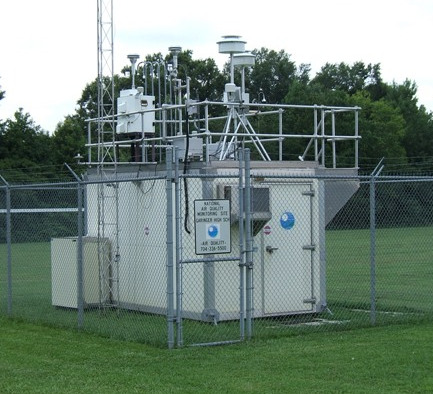
\includegraphics[width=0.5\textwidth]{appendix/sensor_pics/air-monitoring-site.jpg}
\caption{A typical NAAQS-primary grade air quality monitoring station.}
\label{fig:pic-epa-site}
\end{figure}

\begin{figure}[h!]
\centering
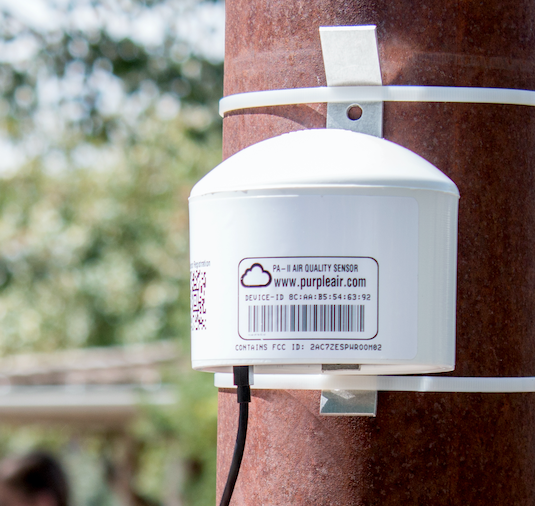
\includegraphics[width=0.5\textwidth]{appendix/sensor_pics/PA_outdoor_monitor.png}
\caption{One of PurpleAir's two main outdoor air pollution monitors.}
\label{fig:pic-ps-sensor}
\end{figure}

\FloatBarrier
\newpage
\subsection{Plots for Other California Hourly NAAQS Monitors} \label{app-additional-plots}



%=========================================
%  Concentric Radii Maps
%=========================================
\begin{figure}[h!]
\centering
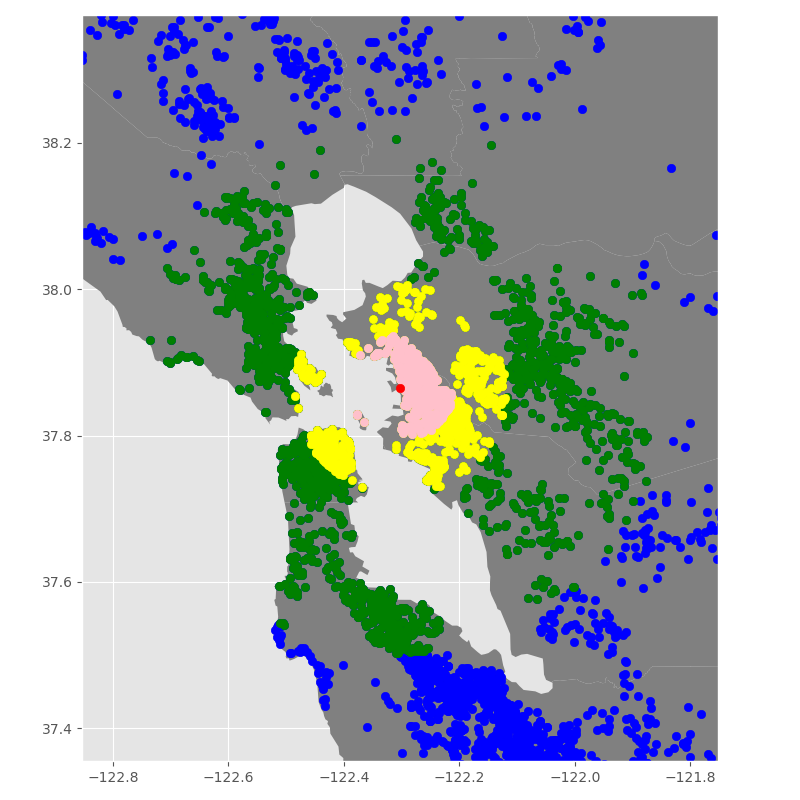
\includegraphics[width=0.8\textwidth]{appendix/site_plots/county-001_site-0013_epa-pa-concentric-ranges.png}
\caption{Map of EPA NAAQS-primary monitoring station (red) surrounded by PurpleAir monitors within 5-mile (pink), 10-mile (yellow), and 25-mile (green) radii.This preliminary analysis uses the PurpleAir sensors within 5 miles (pink markers). This monitor is at site 0013 in county 001 (FIPS code).}
\label{fig:concentric_purpleair_001-0013}
\end{figure}
\begin{figure}
\centering
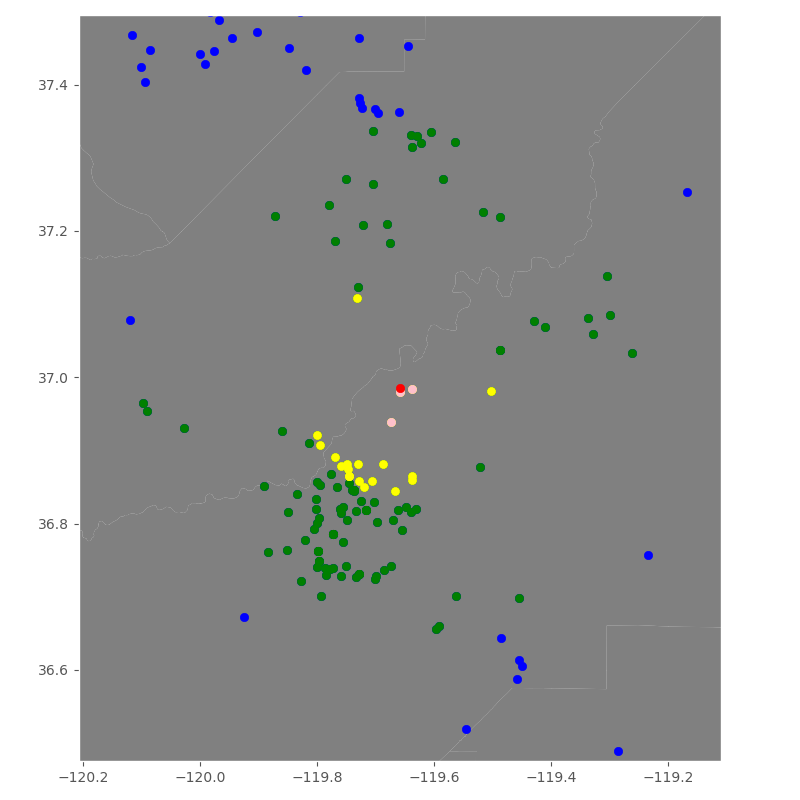
\includegraphics[width=0.8\textwidth]{appendix/site_plots/county-019_site-0500_epa-pa-concentric-ranges.png}
\caption{Map of EPA NAAQS-primary monitoring station (red) surrounded by PurpleAir monitors within 5-mile (pink), 10-mile (yellow), and 25-mile (green) radii.This preliminary analysis uses the PurpleAir sensors within 5 miles (pink markers). This monitor is at site 0500 in county 019 (FIPS code).}
\label{fig:concentric_purpleair_019-0500}
\end{figure}
\begin{figure}
\centering
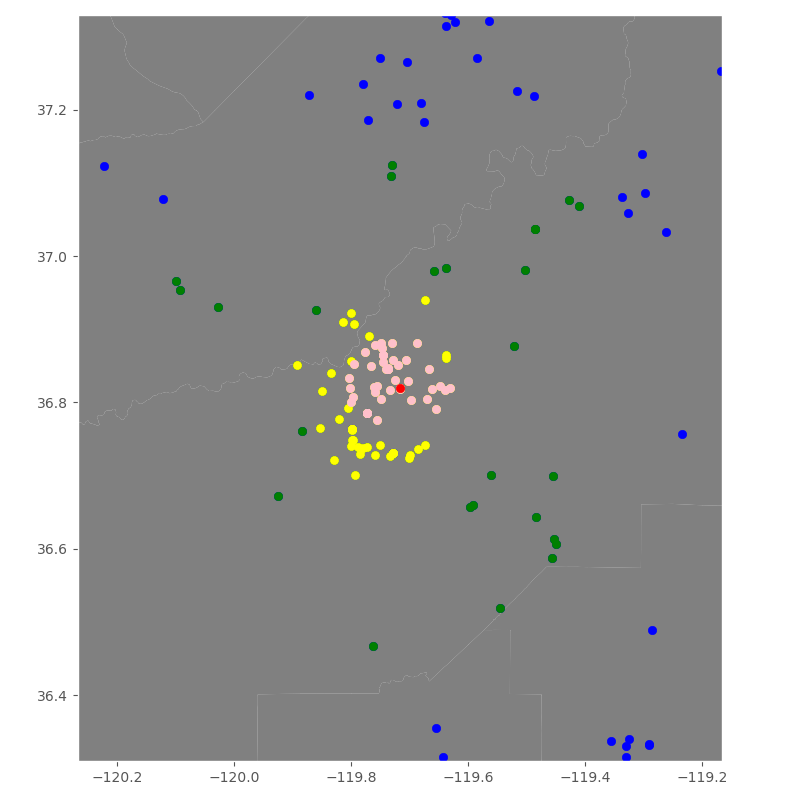
\includegraphics[width=0.8\textwidth]{appendix/site_plots/county-019_site-5001_epa-pa-concentric-ranges.png}
\caption{Map of EPA NAAQS-primary monitoring station (red) surrounded by PurpleAir monitors within 5-mile (pink), 10-mile (yellow), and 25-mile (green) radii.This preliminary analysis uses the PurpleAir sensors within 5 miles (pink markers). This monitor is at site 5001 in county 019 (FIPS code).}
\label{fig:concentric_purpleair_019-5001}
\end{figure}
\begin{figure}
\centering
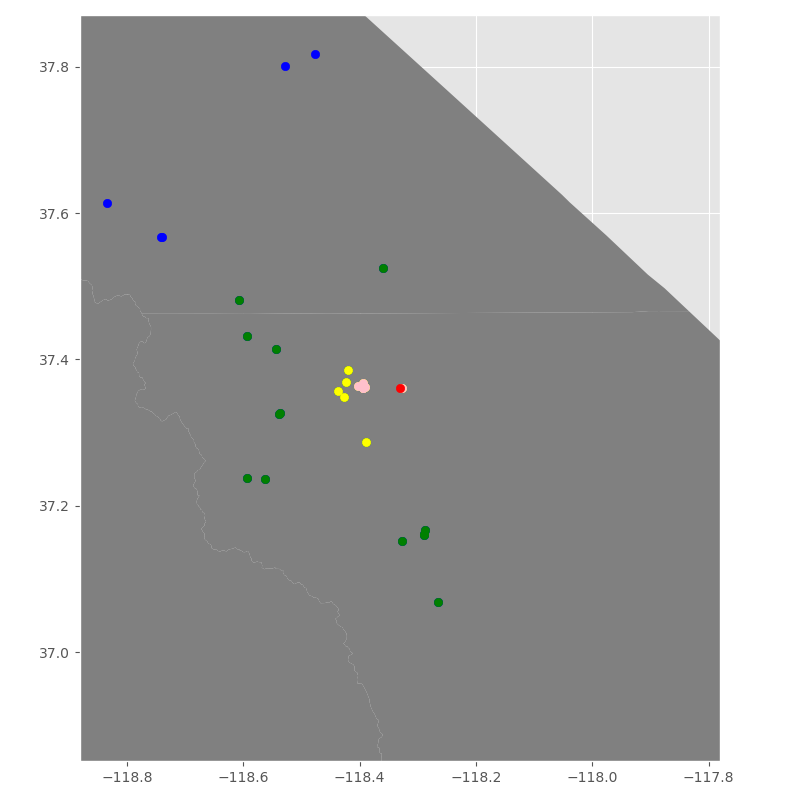
\includegraphics[width=0.8\textwidth]{appendix/site_plots/county-027_site-0002_epa-pa-concentric-ranges.png}
\caption{Map of EPA NAAQS-primary monitoring station (red) surrounded by PurpleAir monitors within 5-mile (pink), 10-mile (yellow), and 25-mile (green) radii.This preliminary analysis uses the PurpleAir sensors within 5 miles (pink markers). This monitor is at site 0002 in county 027 (FIPS code).}
\label{fig:concentric_purpleair_027-0002}
\end{figure}
\begin{figure}
\centering
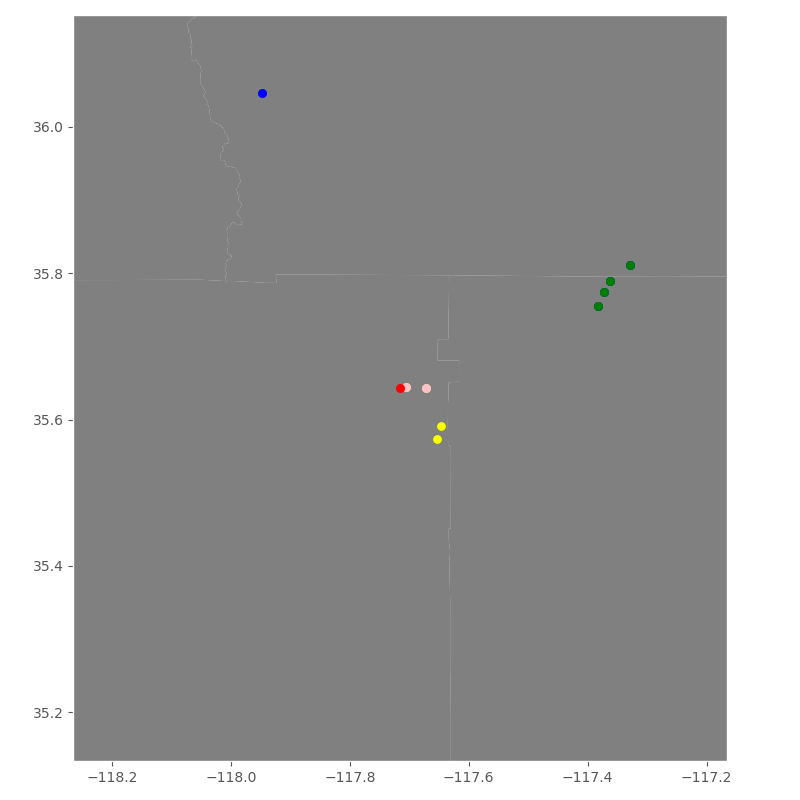
\includegraphics[width=0.8\textwidth]{appendix/site_plots/county-029_site-0018_epa-pa-concentric-ranges.png}
\caption{Map of EPA NAAQS-primary monitoring station (red) surrounded by PurpleAir monitors within 5-mile (pink), 10-mile (yellow), and 25-mile (green) radii.This preliminary analysis uses the PurpleAir sensors within 5 miles (pink markers). This monitor is at site 0018 in county 029 (FIPS code).}
\label{fig:concentric_purpleair_029-0018}
\end{figure}
\begin{figure}
\centering
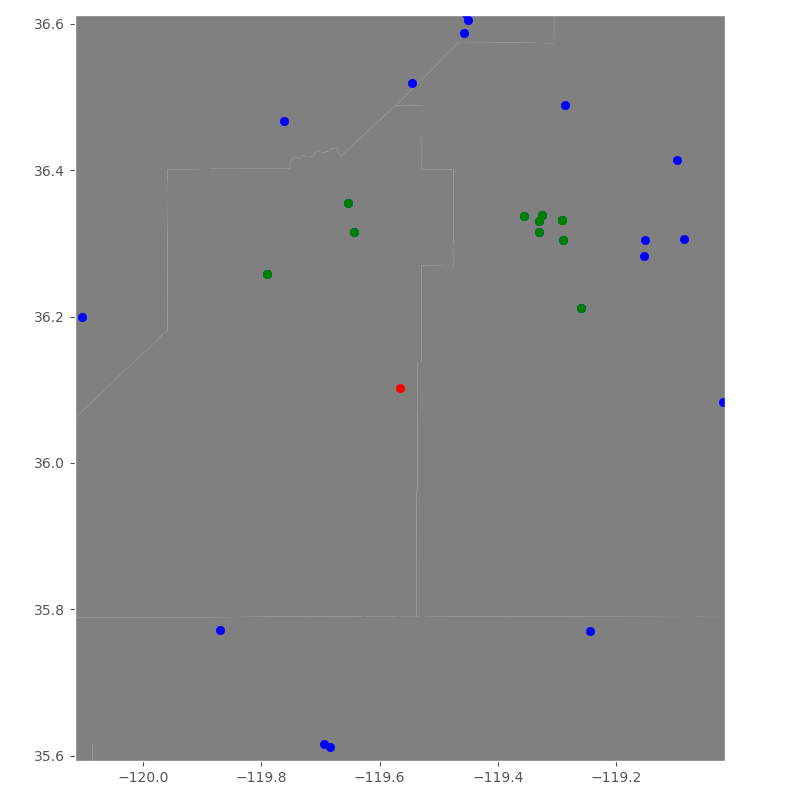
\includegraphics[width=0.8\textwidth]{appendix/site_plots/county-031_site-0004_epa-pa-concentric-ranges.png}
\caption{Map of EPA NAAQS-primary monitoring station (red) surrounded by PurpleAir monitors within 5-mile (pink), 10-mile (yellow), and 25-mile (green) radii.This preliminary analysis uses the PurpleAir sensors within 5 miles (pink markers). This monitor is at site 0004 in county 031 (FIPS code).}
\label{fig:concentric_purpleair_031-0004}
\end{figure}
\begin{figure}
\centering
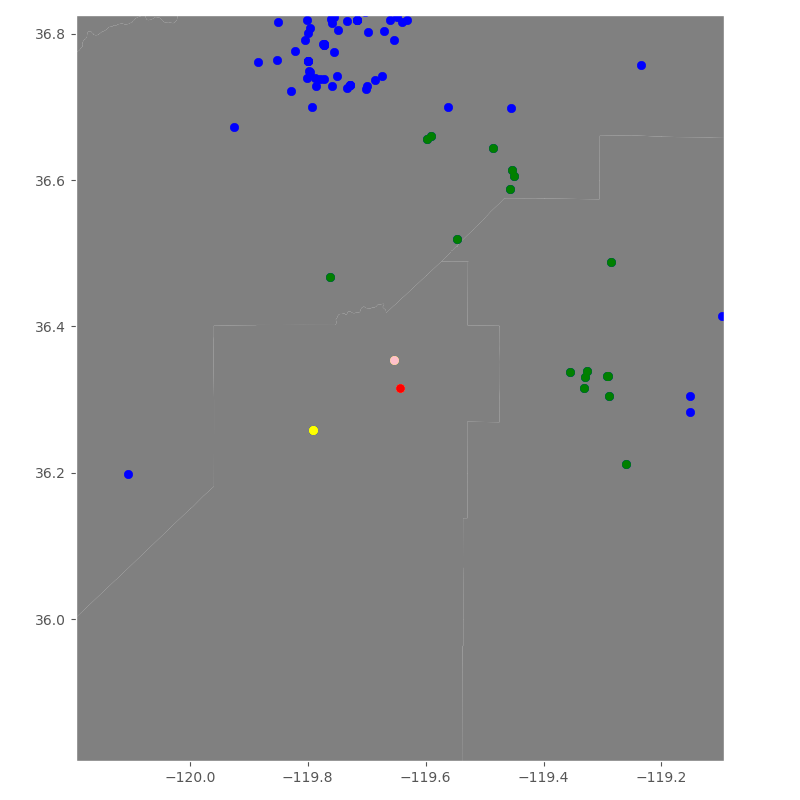
\includegraphics[width=0.8\textwidth]{appendix/site_plots/county-031_site-1004_epa-pa-concentric-ranges.png}
\caption{Map of EPA NAAQS-primary monitoring station (red) surrounded by PurpleAir monitors within 5-mile (pink), 10-mile (yellow), and 25-mile (green) radii.This preliminary analysis uses the PurpleAir sensors within 5 miles (pink markers). This monitor is at site 1004 in county 031 (FIPS code).}
\label{fig:concentric_purpleair_031-1004}
\end{figure}
\begin{figure}
\centering
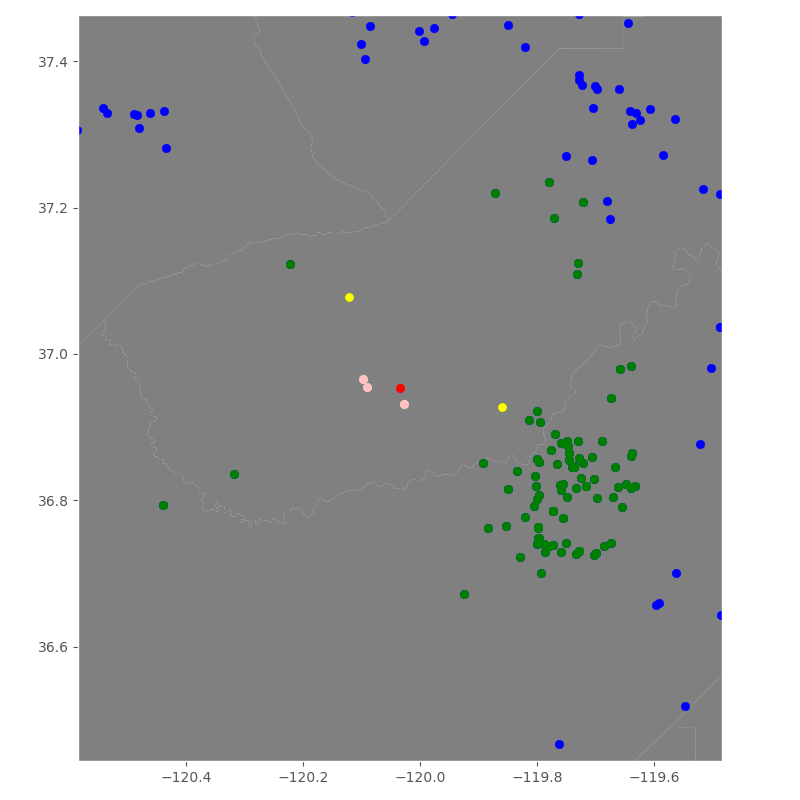
\includegraphics[width=0.8\textwidth]{appendix/site_plots/county-039_site-2010_epa-pa-concentric-ranges.png}
\caption{Map of EPA NAAQS-primary monitoring station (red) surrounded by PurpleAir monitors within 5-mile (pink), 10-mile (yellow), and 25-mile (green) radii.This preliminary analysis uses the PurpleAir sensors within 5 miles (pink markers). This monitor is at site 2010 in county 039 (FIPS code).}
\label{fig:concentric_purpleair_039-2010}
\end{figure}
\begin{figure}
\centering
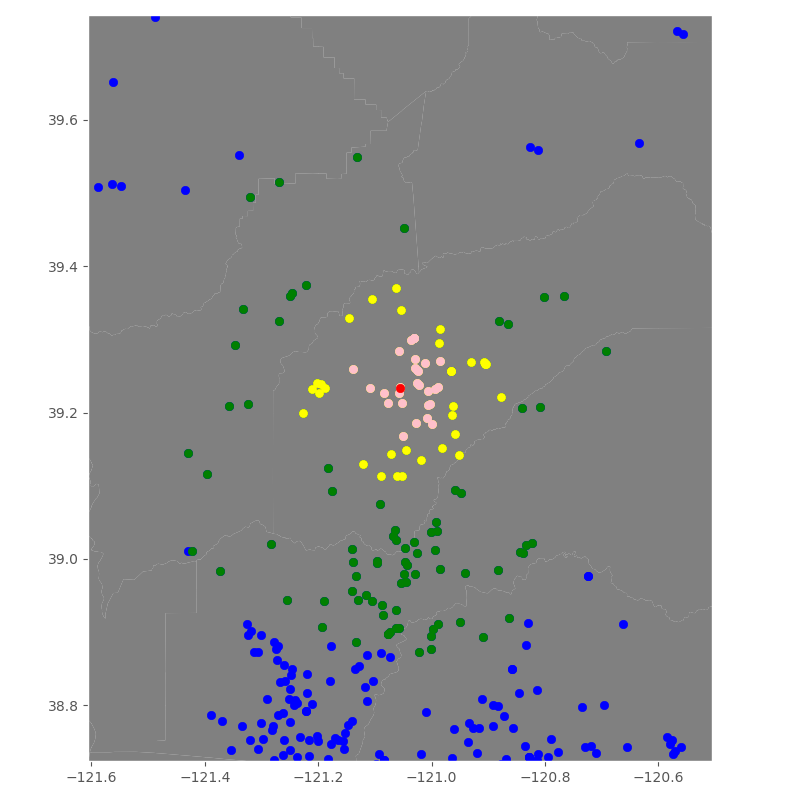
\includegraphics[width=0.8\textwidth]{appendix/site_plots/county-057_site-0005_epa-pa-concentric-ranges.png}
\caption{Map of EPA NAAQS-primary monitoring station (red) surrounded by PurpleAir monitors within 5-mile (pink), 10-mile (yellow), and 25-mile (green) radii.This preliminary analysis uses the PurpleAir sensors within 5 miles (pink markers). This monitor is at site 0005 in county 057 (FIPS code).}
\label{fig:concentric_purpleair_057-0005}
\end{figure}
\begin{figure}
\centering
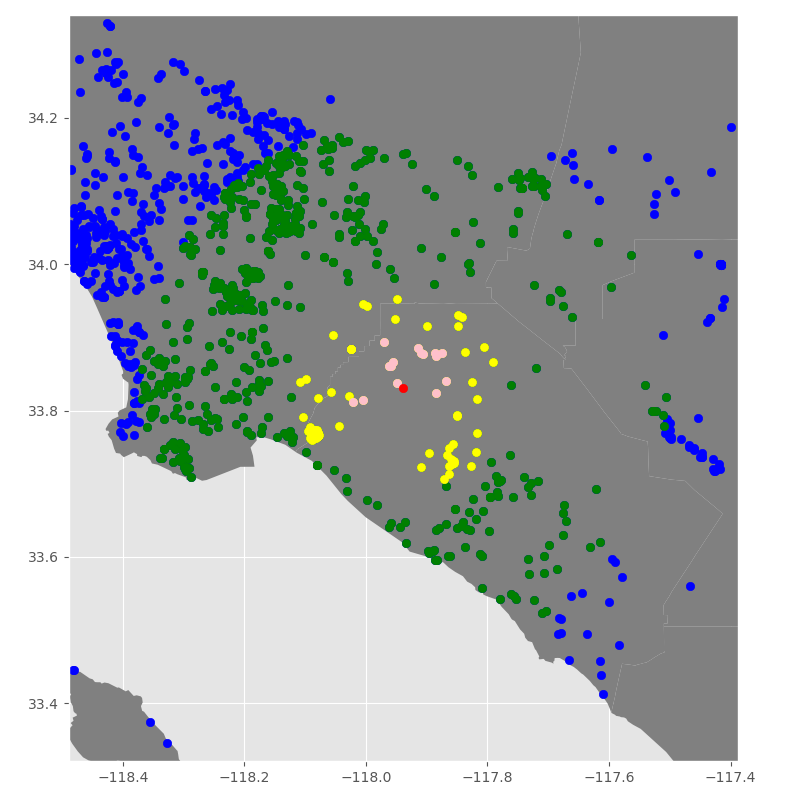
\includegraphics[width=0.8\textwidth]{appendix/site_plots/county-059_site-0007_epa-pa-concentric-ranges.png}
\caption{Map of EPA NAAQS-primary monitoring station (red) surrounded by PurpleAir monitors within 5-mile (pink), 10-mile (yellow), and 25-mile (green) radii.This preliminary analysis uses the PurpleAir sensors within 5 miles (pink markers). This monitor is at site 0007 in county 059 (FIPS code).}
\label{fig:concentric_purpleair_059-0007}
\end{figure}
\begin{figure}
\centering
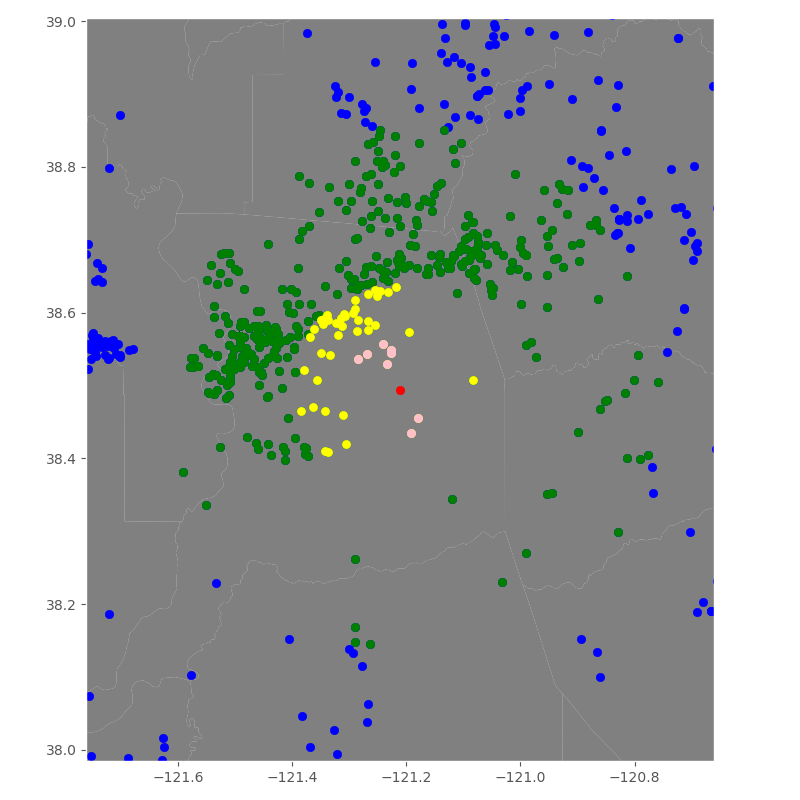
\includegraphics[width=0.8\textwidth]{appendix/site_plots/county-067_site-5003_epa-pa-concentric-ranges.png}
\caption{Map of EPA NAAQS-primary monitoring station (red) surrounded by PurpleAir monitors within 5-mile (pink), 10-mile (yellow), and 25-mile (green) radii.This preliminary analysis uses the PurpleAir sensors within 5 miles (pink markers). This monitor is at site 5003 in county 067 (FIPS code).}
\label{fig:concentric_purpleair_067-5003}
\end{figure}
\begin{figure}
\centering
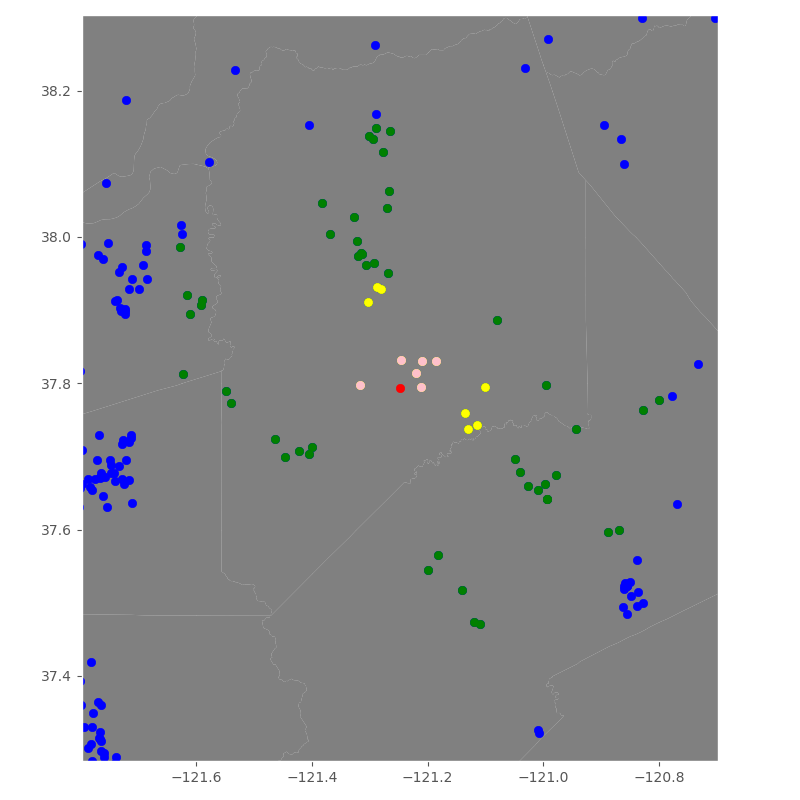
\includegraphics[width=0.8\textwidth]{appendix/site_plots/county-077_site-2010_epa-pa-concentric-ranges.png}
\caption{Map of EPA NAAQS-primary monitoring station (red) surrounded by PurpleAir monitors within 5-mile (pink), 10-mile (yellow), and 25-mile (green) radii.This preliminary analysis uses the PurpleAir sensors within 5 miles (pink markers). This monitor is at site 2010 in county 077 (FIPS code).}
\label{fig:concentric_purpleair_077-2010}
\end{figure}
\begin{figure}
\centering
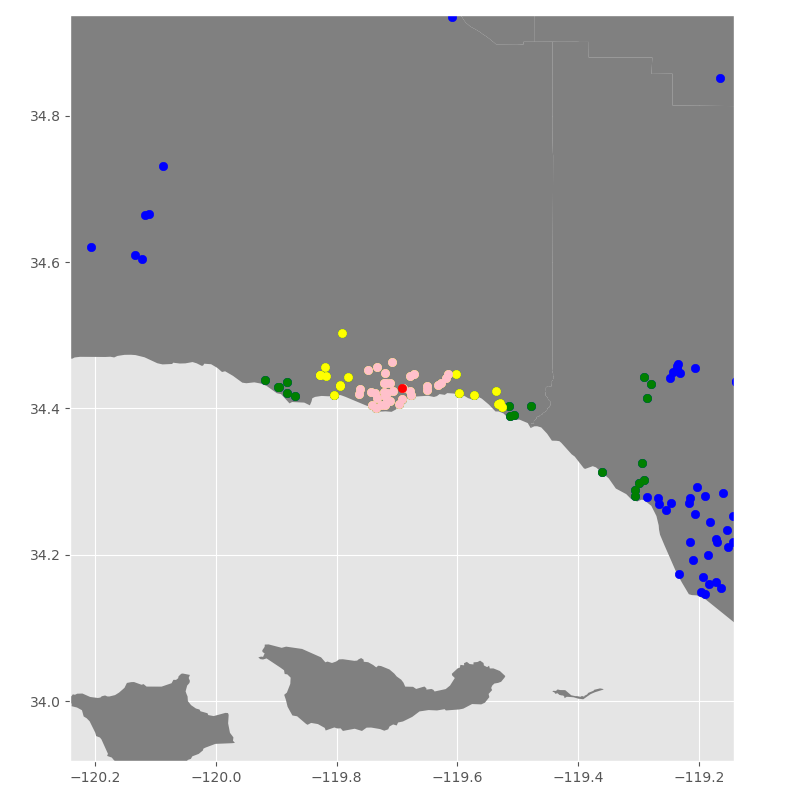
\includegraphics[width=0.8\textwidth]{appendix/site_plots/county-083_site-0011_epa-pa-concentric-ranges.png}
\caption{Map of EPA NAAQS-primary monitoring station (red) surrounded by PurpleAir monitors within 5-mile (pink), 10-mile (yellow), and 25-mile (green) radii.This preliminary analysis uses the PurpleAir sensors within 5 miles (pink markers). This monitor is at site 0011 in county 083 (FIPS code).}
\label{fig:concentric_purpleair_083-0011}
\end{figure}
\begin{figure}
\centering
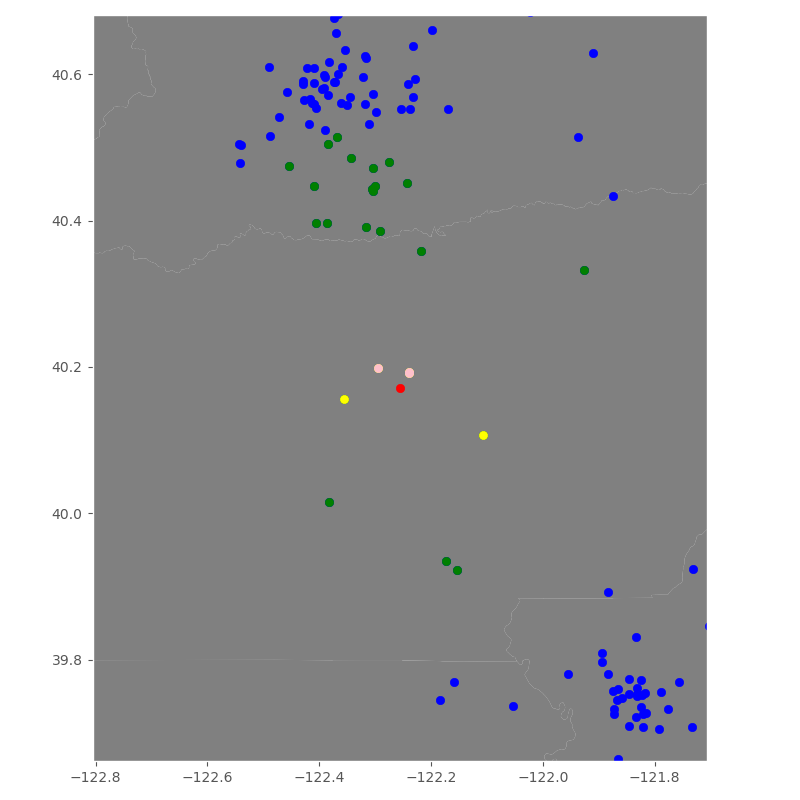
\includegraphics[width=0.8\textwidth]{appendix/site_plots/county-103_site-0007_epa-pa-concentric-ranges.png}
\caption{Map of EPA NAAQS-primary monitoring station (red) surrounded by PurpleAir monitors within 5-mile (pink), 10-mile (yellow), and 25-mile (green) radii.This preliminary analysis uses the PurpleAir sensors within 5 miles (pink markers). This monitor is at site 0007 in county 103 (FIPS code).}
\label{fig:concentric_purpleair_103-0007}
\end{figure}
%=========================================
%  PurpleAir Hourly Observation Coverage
%=========================================
\begin{figure}
\centering
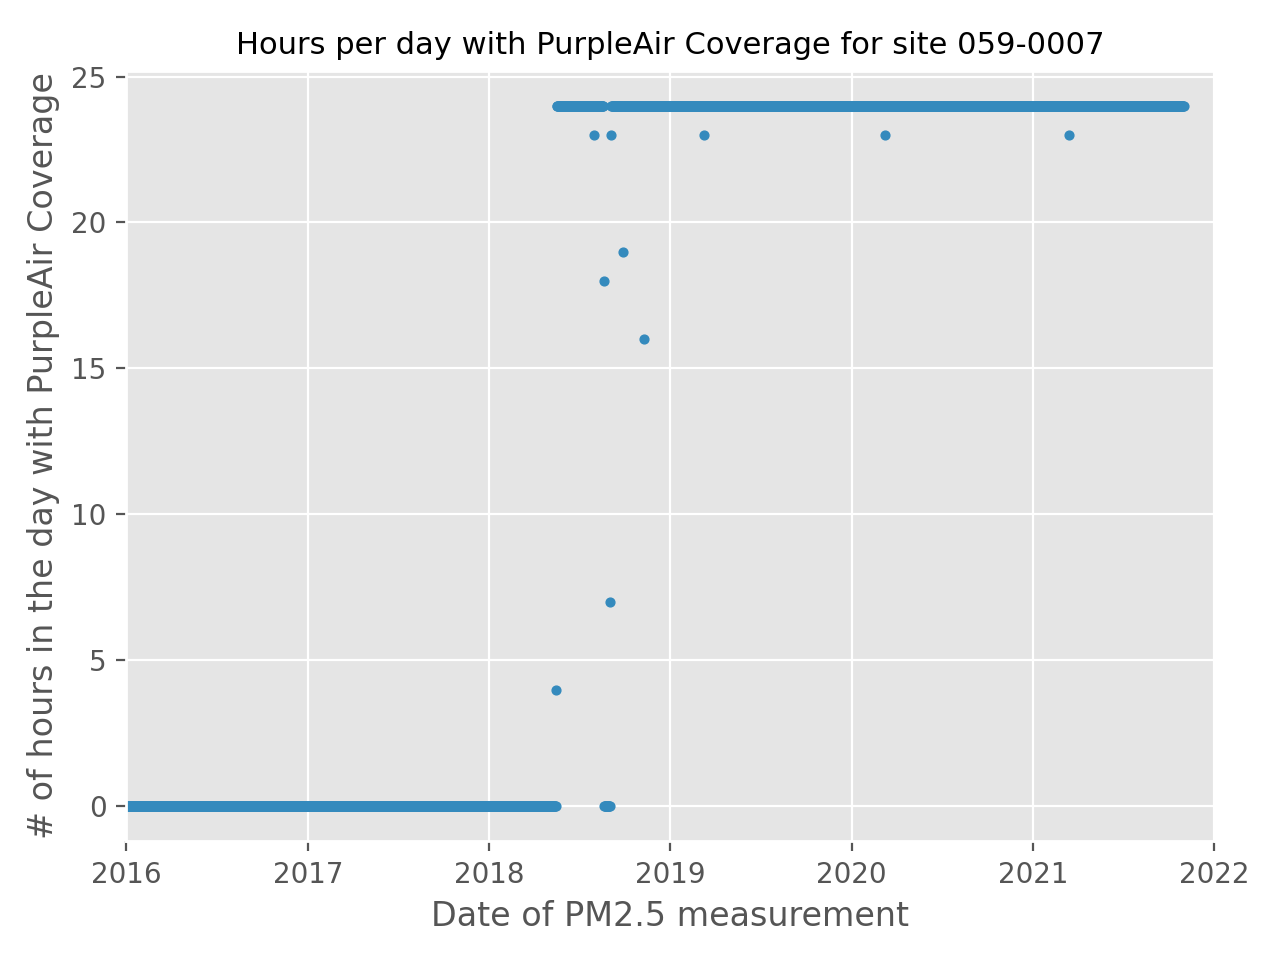
\includegraphics[width=0.8\textwidth]{appendix/site_plots/site-059-0007_pa-daily-covereage.png}
\caption{Scatter plot indicating the number of hours in each day that this NAAQS monitor has PurpleAir coverage. An hour has PurpleAir coverage if there are any PurpleAir sensor readings within the 5-mile radius of the monitor site for that hour. The weighted average is calculated for that hour using all the available PurpleAir readings within 5 miles. This monitor is at site 0007 in county 059 (FIPS code).}
\label{fig:hourly_coverage_059-0007}
\end{figure}
\begin{figure}
\centering
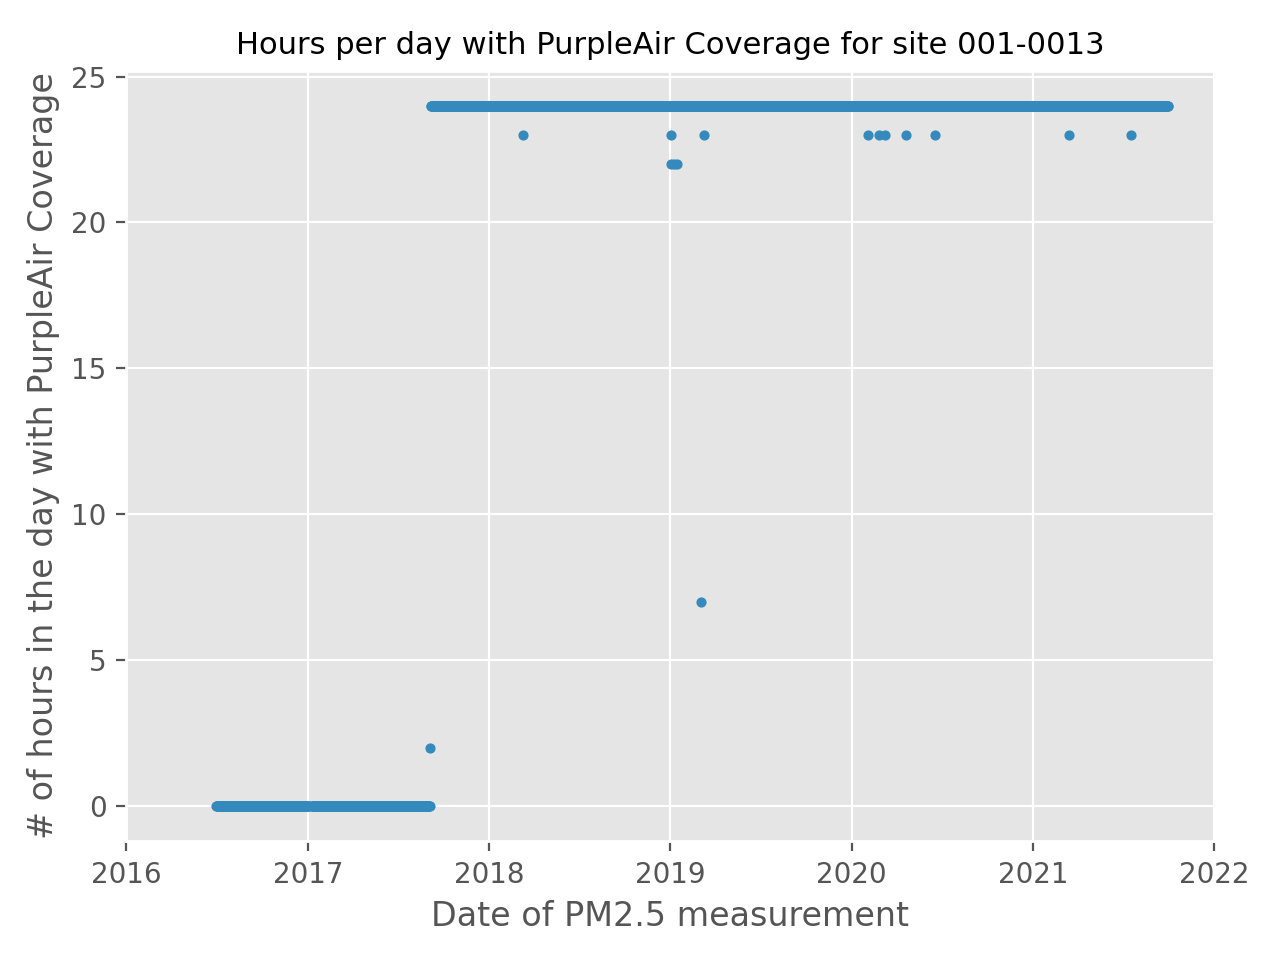
\includegraphics[width=0.8\textwidth]{appendix/site_plots/site-001-0013_pa-daily-covereage.png}
\caption{Scatter plot indicating the number of hours in each day that this NAAQS monitor has PurpleAir coverage. An hour has PurpleAir coverage if there are any PurpleAir sensor readings within the 5-mile radius of the monitor site for that hour. The weighted average is calculated for that hour using all the available PurpleAir readings within 5 miles. This monitor is at site 0013 in county 001 (FIPS code).}
\label{fig:hourly_coverage_001-0013}
\end{figure}
\begin{figure}
\centering
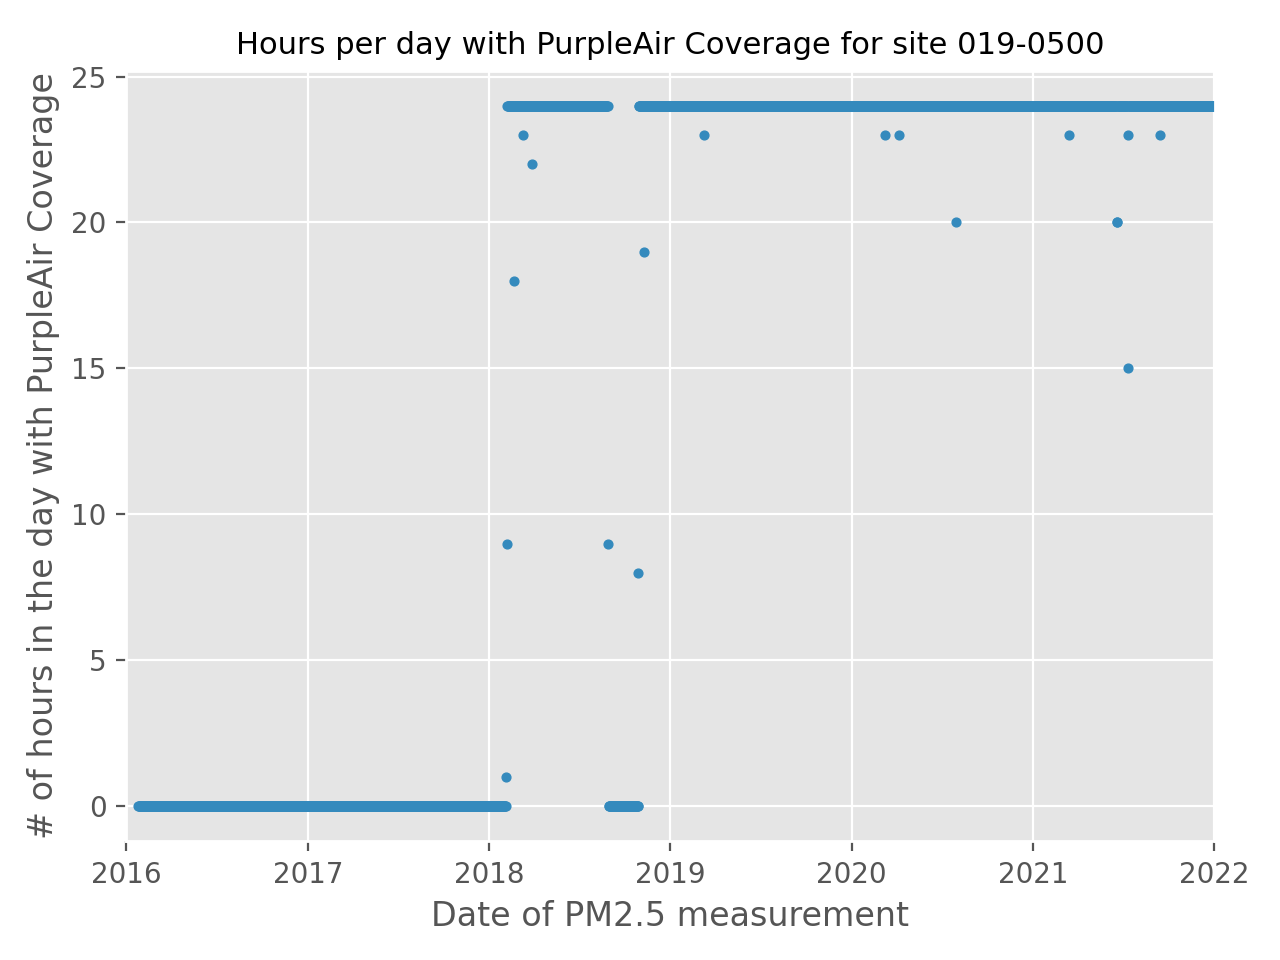
\includegraphics[width=0.8\textwidth]{appendix/site_plots/site-019-0500_pa-daily-covereage.png}
\caption{Scatter plot indicating the number of hours in each day that this NAAQS monitor has PurpleAir coverage. An hour has PurpleAir coverage if there are any PurpleAir sensor readings within the 5-mile radius of the monitor site for that hour. The weighted average is calculated for that hour using all the available PurpleAir readings within 5 miles. This monitor is at site 0500 in county 019 (FIPS code).}
\label{fig:hourly_coverage_019-0500}
\end{figure}
\begin{figure}
\centering
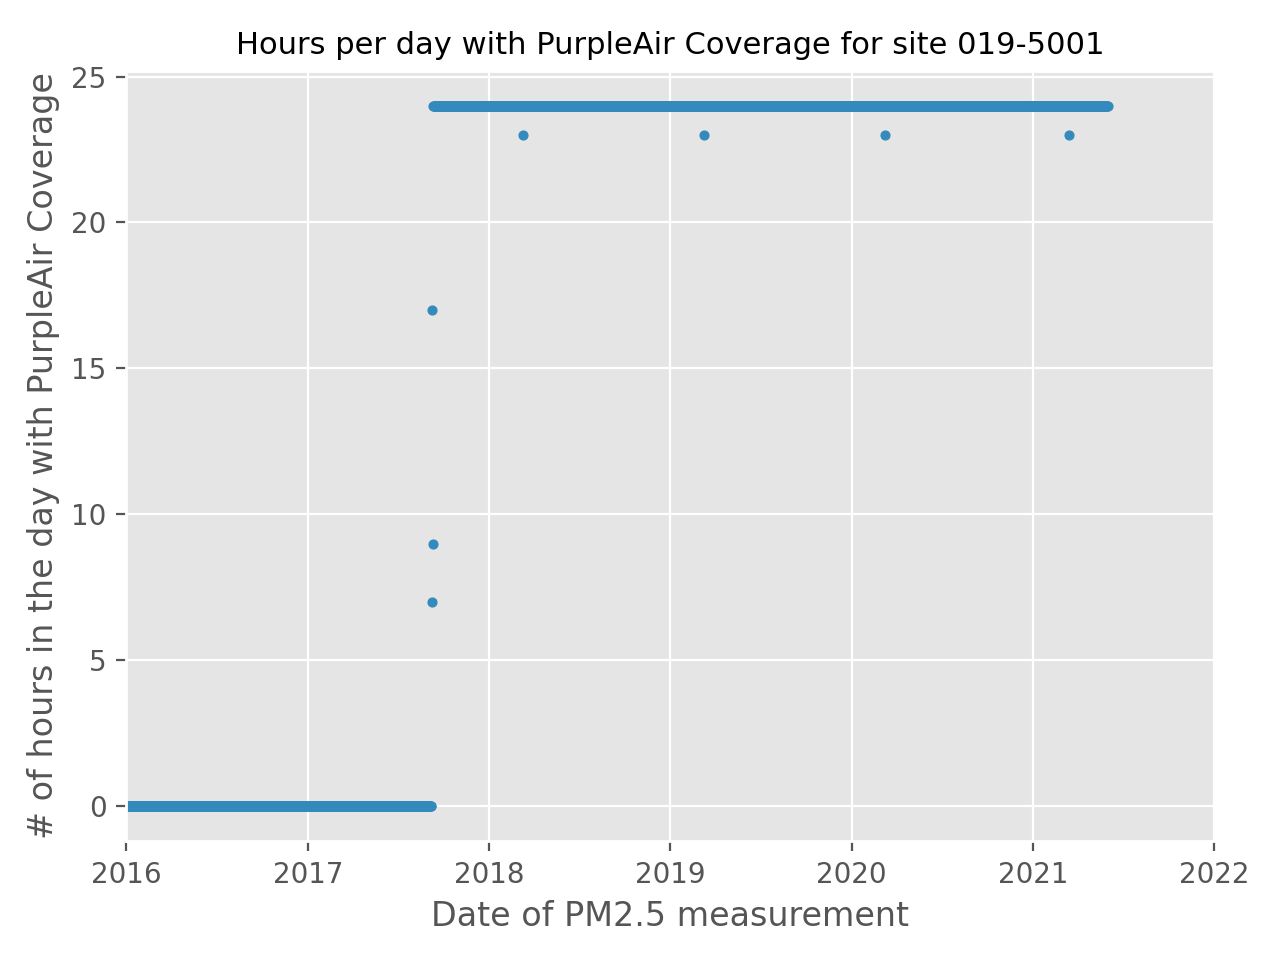
\includegraphics[width=0.8\textwidth]{appendix/site_plots/site-019-5001_pa-daily-covereage.png}
\caption{Scatter plot indicating the number of hours in each day that this NAAQS monitor has PurpleAir coverage. An hour has PurpleAir coverage if there are any PurpleAir sensor readings within the 5-mile radius of the monitor site for that hour. The weighted average is calculated for that hour using all the available PurpleAir readings within 5 miles. This monitor is at site 5001 in county 019 (FIPS code).}
\label{fig:hourly_coverage_019-5001}
\end{figure}
\begin{figure}
\centering
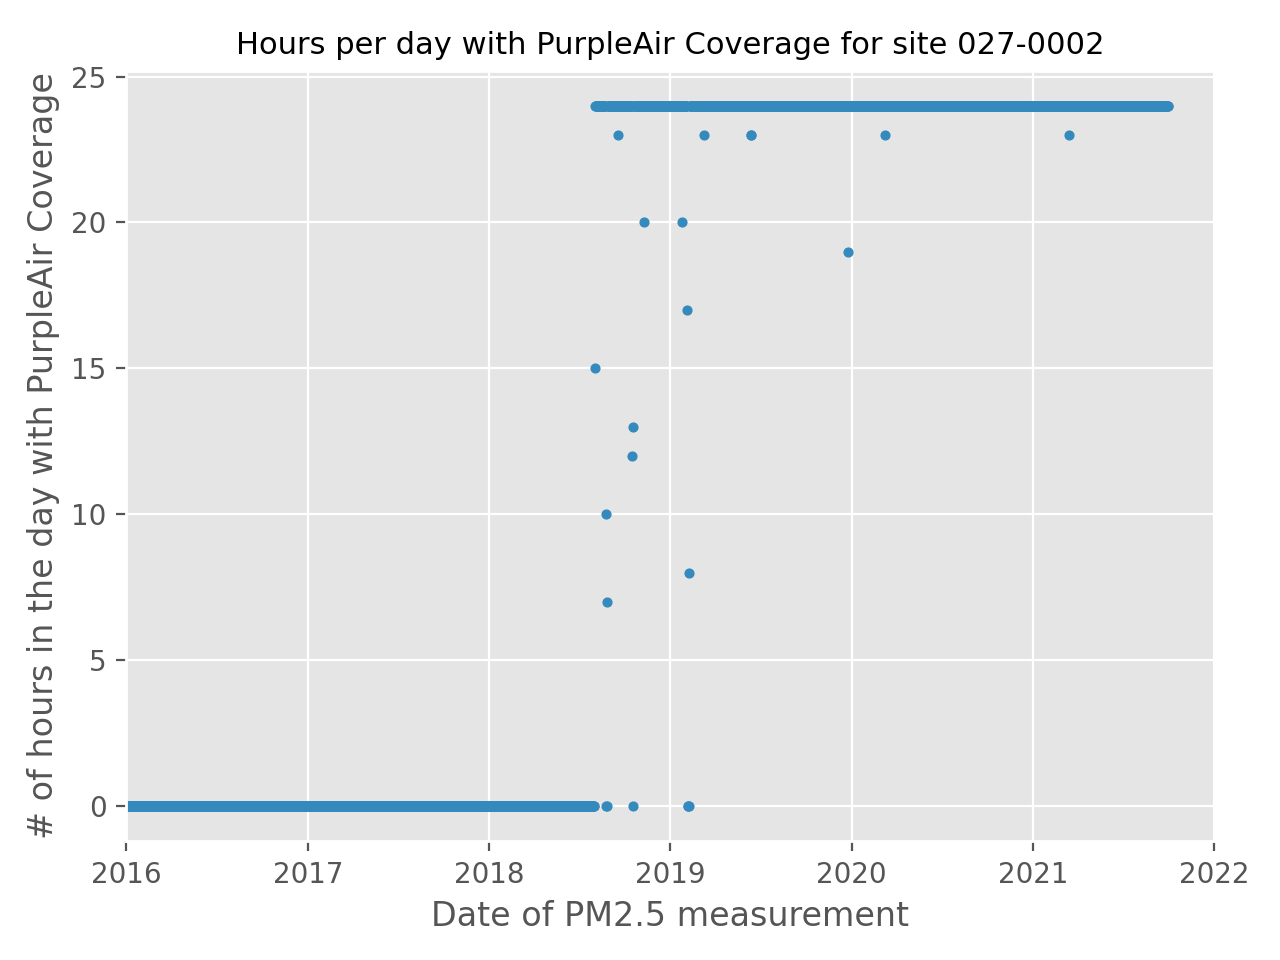
\includegraphics[width=0.8\textwidth]{appendix/site_plots/site-027-0002_pa-daily-covereage.png}
\caption{Scatter plot indicating the number of hours in each day that this NAAQS monitor has PurpleAir coverage. An hour has PurpleAir coverage if there are any PurpleAir sensor readings within the 5-mile radius of the monitor site for that hour. The weighted average is calculated for that hour using all the available PurpleAir readings within 5 miles. This monitor is at site 0002 in county 027 (FIPS code).}
\label{fig:hourly_coverage_027-0002}
\end{figure}
\begin{figure}
\centering
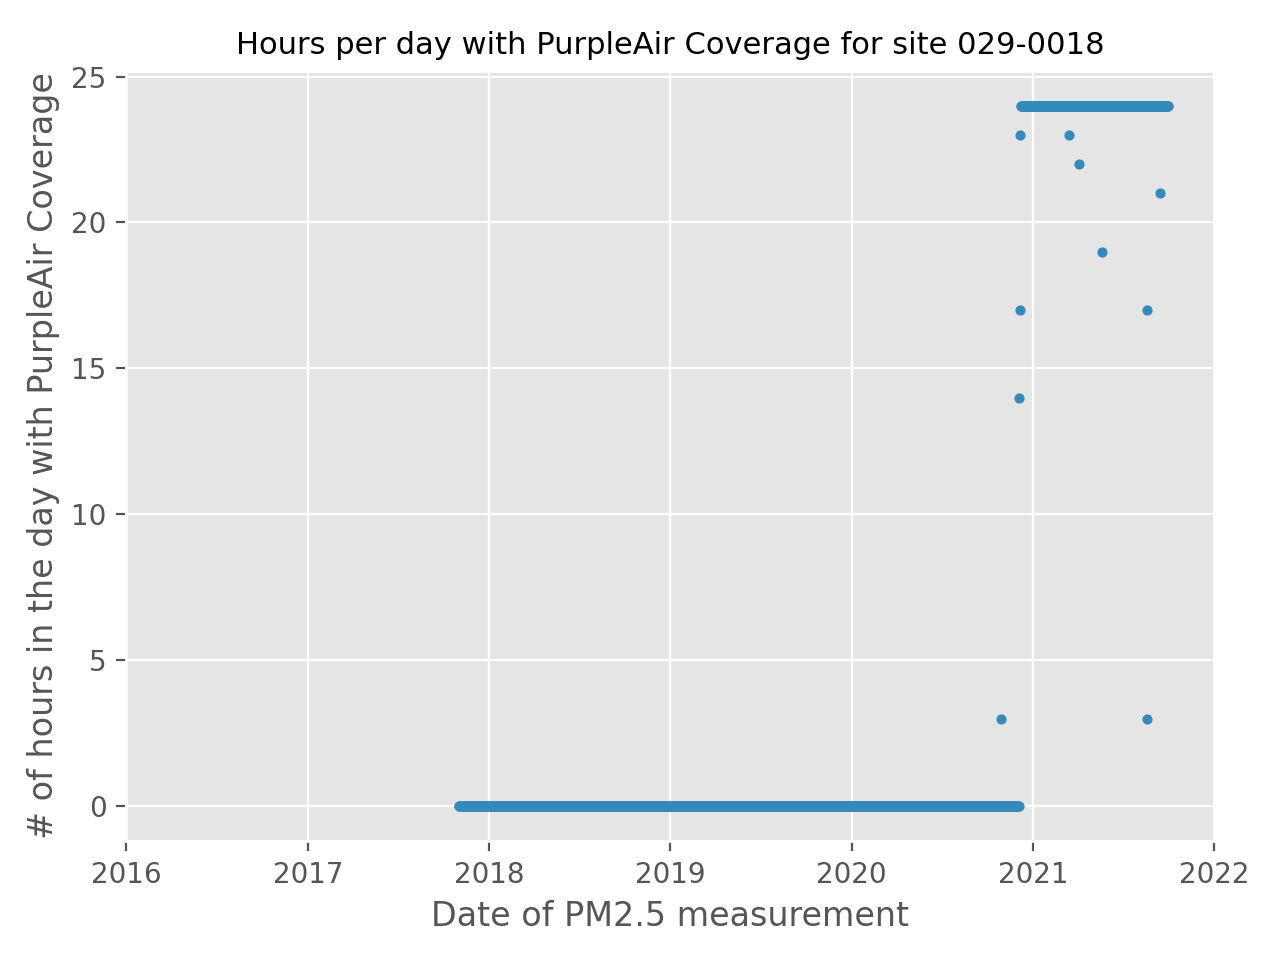
\includegraphics[width=0.8\textwidth]{appendix/site_plots/site-029-0018_pa-daily-covereage.png}
\caption{Scatter plot indicating the number of hours in each day that this NAAQS monitor has PurpleAir coverage. An hour has PurpleAir coverage if there are any PurpleAir sensor readings within the 5-mile radius of the monitor site for that hour. The weighted average is calculated for that hour using all the available PurpleAir readings within 5 miles. This monitor is at site 0018 in county 029 (FIPS code).}
\label{fig:hourly_coverage_029-0018}
\end{figure}
\begin{figure}
\centering
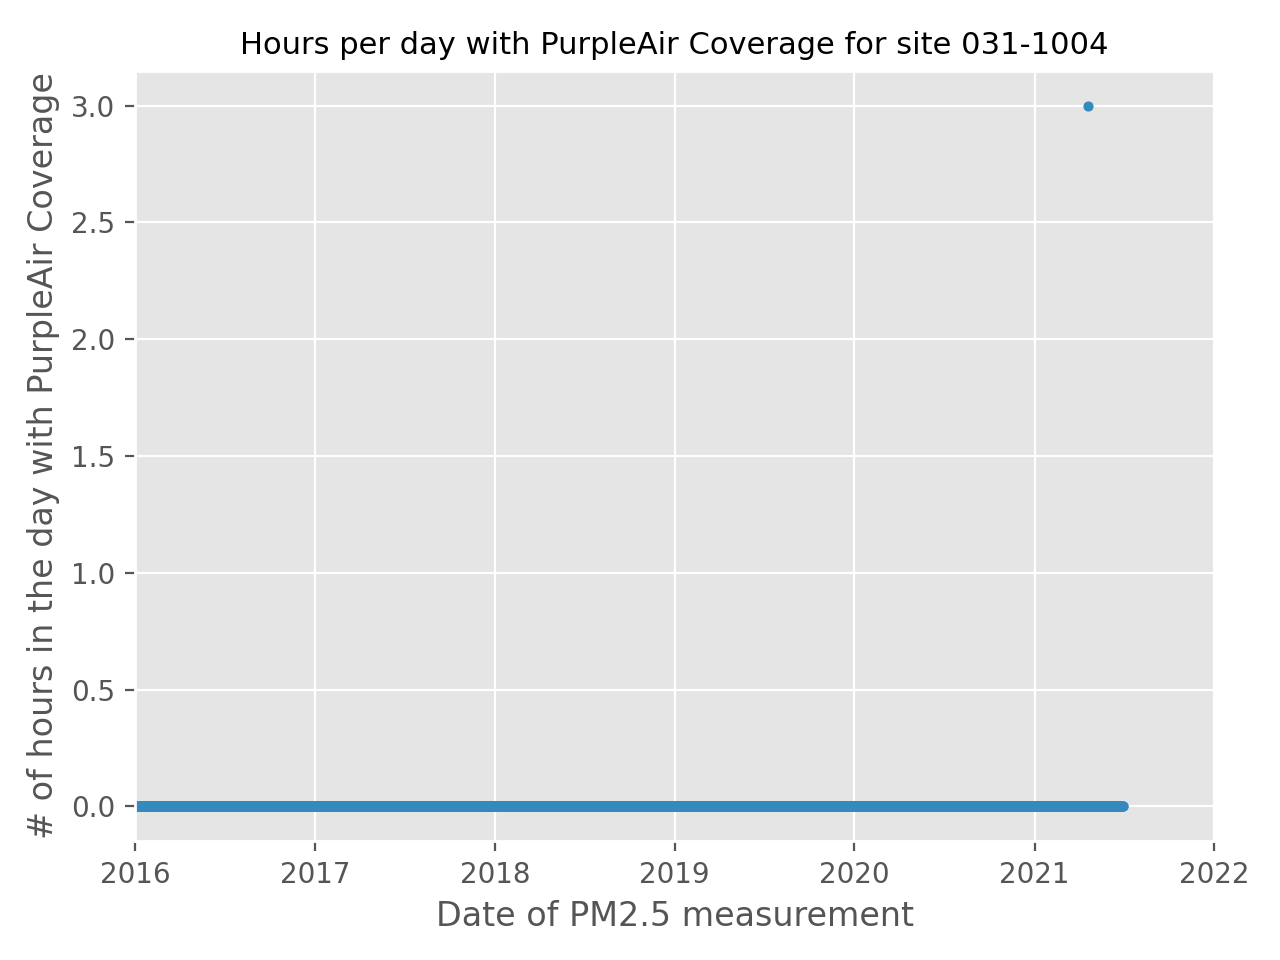
\includegraphics[width=0.8\textwidth]{appendix/site_plots/site-031-1004_pa-daily-covereage.png}
\caption{Scatter plot indicating the number of hours in each day that this NAAQS monitor has PurpleAir coverage. An hour has PurpleAir coverage if there are any PurpleAir sensor readings within the 5-mile radius of the monitor site for that hour. The weighted average is calculated for that hour using all the available PurpleAir readings within 5 miles. This monitor is at site 1004 in county 031 (FIPS code).}
\label{fig:hourly_coverage_031-1004}
\end{figure}
\begin{figure}
\centering
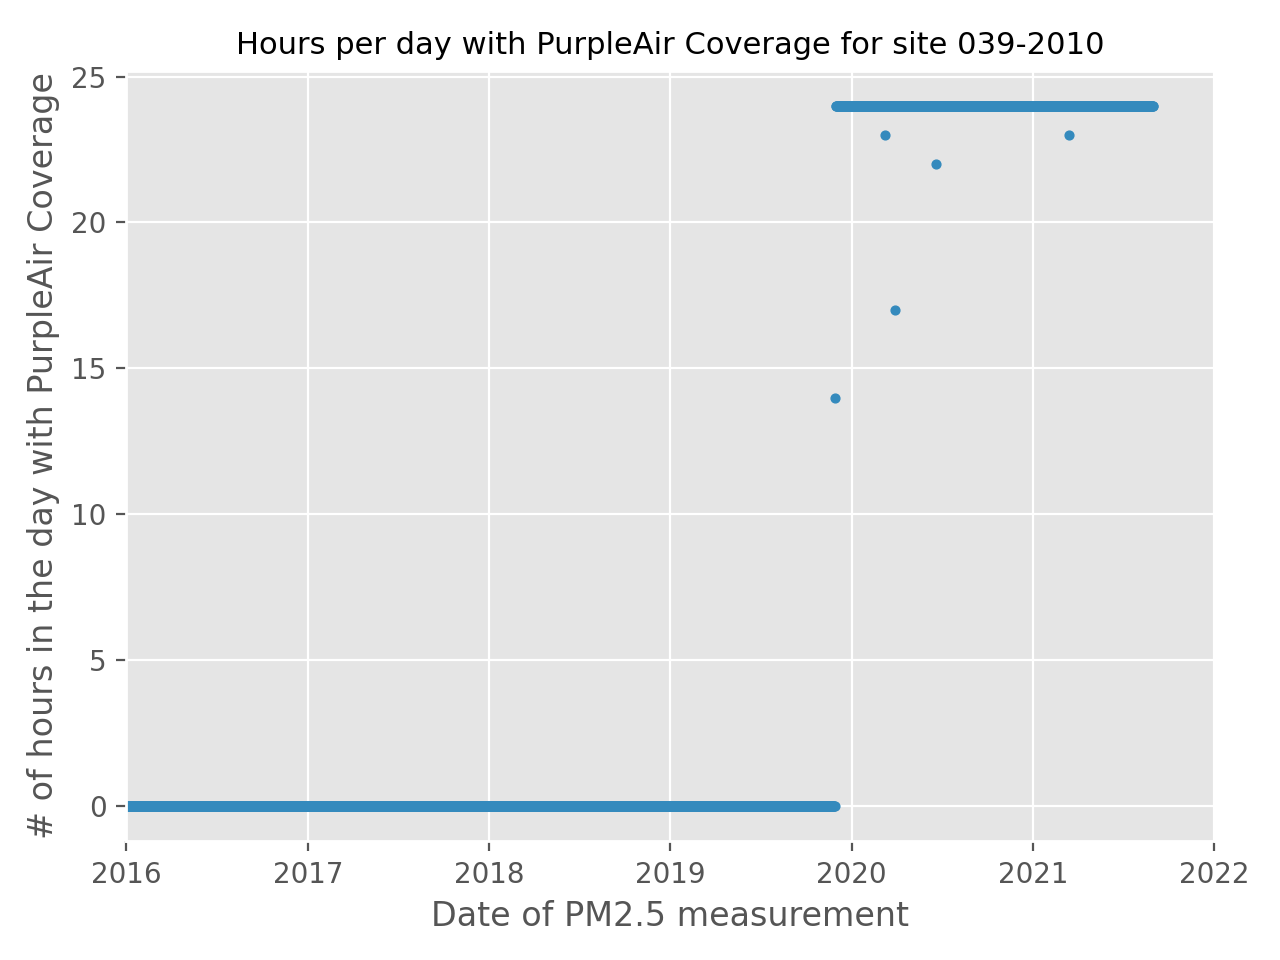
\includegraphics[width=0.8\textwidth]{appendix/site_plots/site-039-2010_pa-daily-covereage.png}
\caption{Scatter plot indicating the number of hours in each day that this NAAQS monitor has PurpleAir coverage. An hour has PurpleAir coverage if there are any PurpleAir sensor readings within the 5-mile radius of the monitor site for that hour. The weighted average is calculated for that hour using all the available PurpleAir readings within 5 miles. This monitor is at site 2010 in county 039 (FIPS code).}
\label{fig:hourly_coverage_039-2010}
\end{figure}
\begin{figure}
\centering
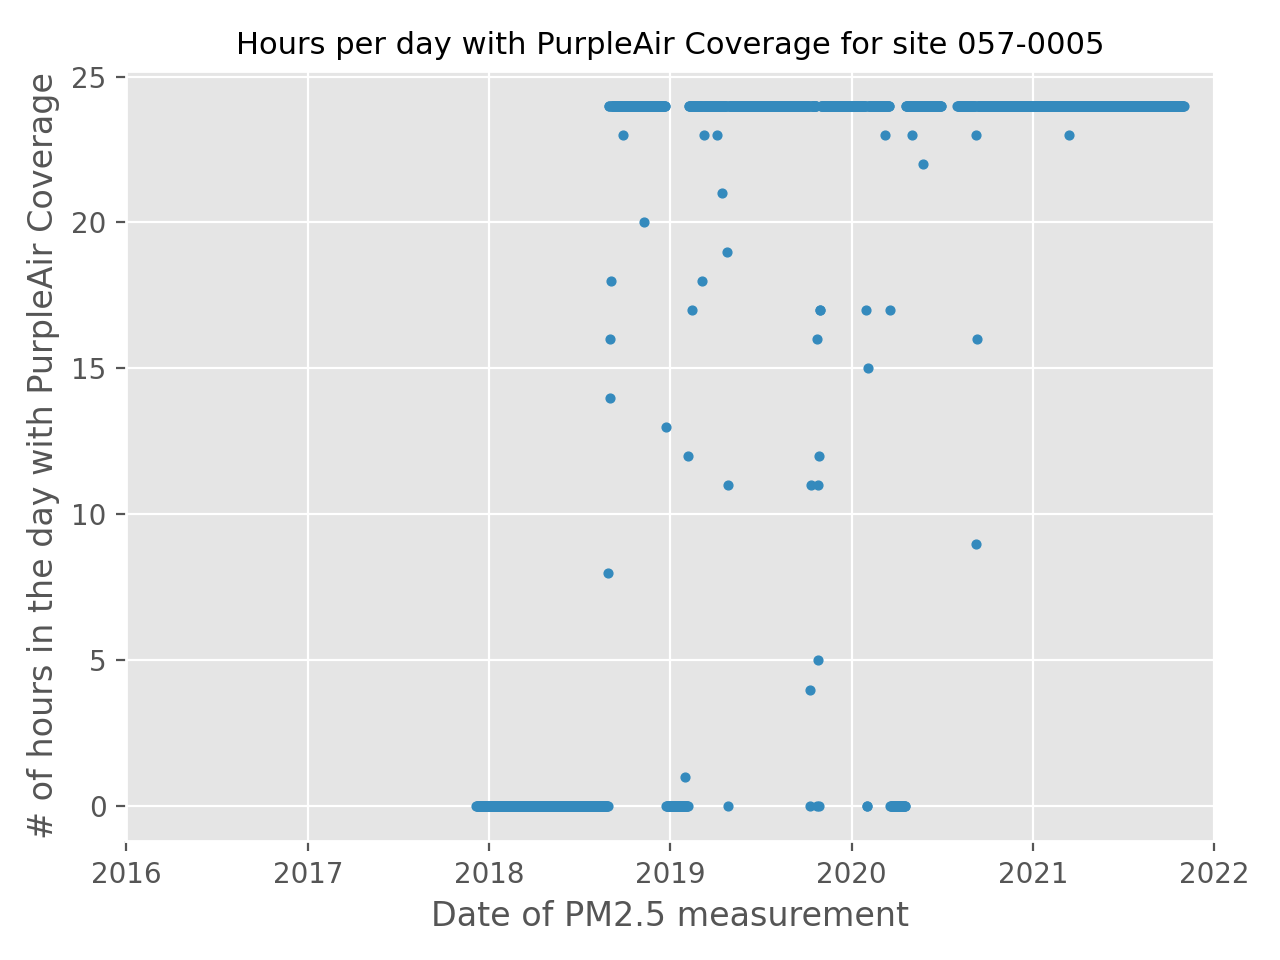
\includegraphics[width=0.8\textwidth]{appendix/site_plots/site-057-0005_pa-daily-covereage.png}
\caption{Scatter plot indicating the number of hours in each day that this NAAQS monitor has PurpleAir coverage. An hour has PurpleAir coverage if there are any PurpleAir sensor readings within the 5-mile radius of the monitor site for that hour. The weighted average is calculated for that hour using all the available PurpleAir readings within 5 miles. This monitor is at site 0005 in county 057 (FIPS code).}
\label{fig:hourly_coverage_057-0005}
\end{figure}
\begin{figure}
\centering
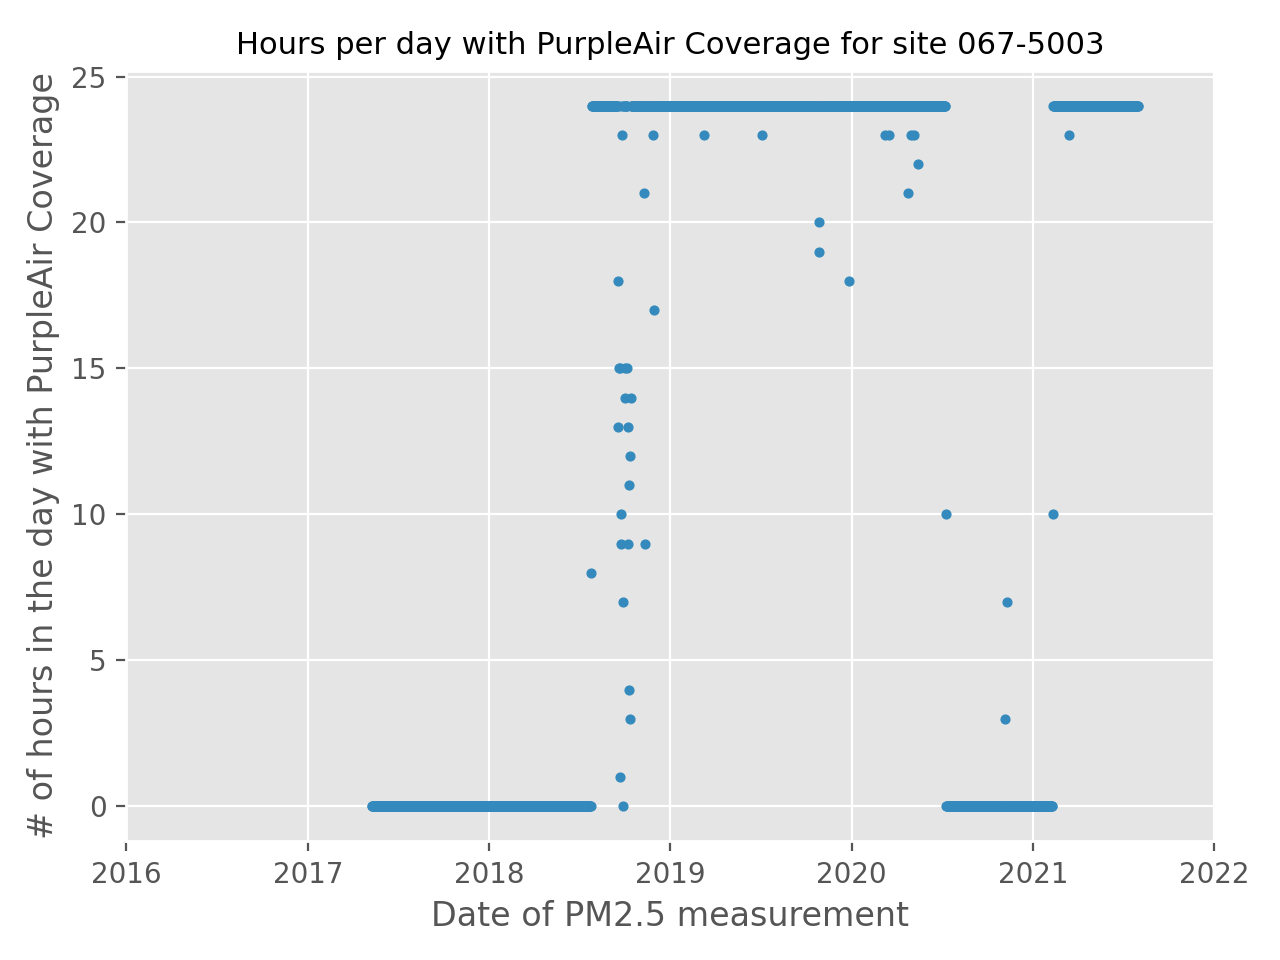
\includegraphics[width=0.8\textwidth]{appendix/site_plots/site-067-5003_pa-daily-covereage.png}
\caption{Scatter plot indicating the number of hours in each day that this NAAQS monitor has PurpleAir coverage. An hour has PurpleAir coverage if there are any PurpleAir sensor readings within the 5-mile radius of the monitor site for that hour. The weighted average is calculated for that hour using all the available PurpleAir readings within 5 miles. This monitor is at site 5003 in county 067 (FIPS code).}
\label{fig:hourly_coverage_067-5003}
\end{figure}
\begin{figure}
\centering
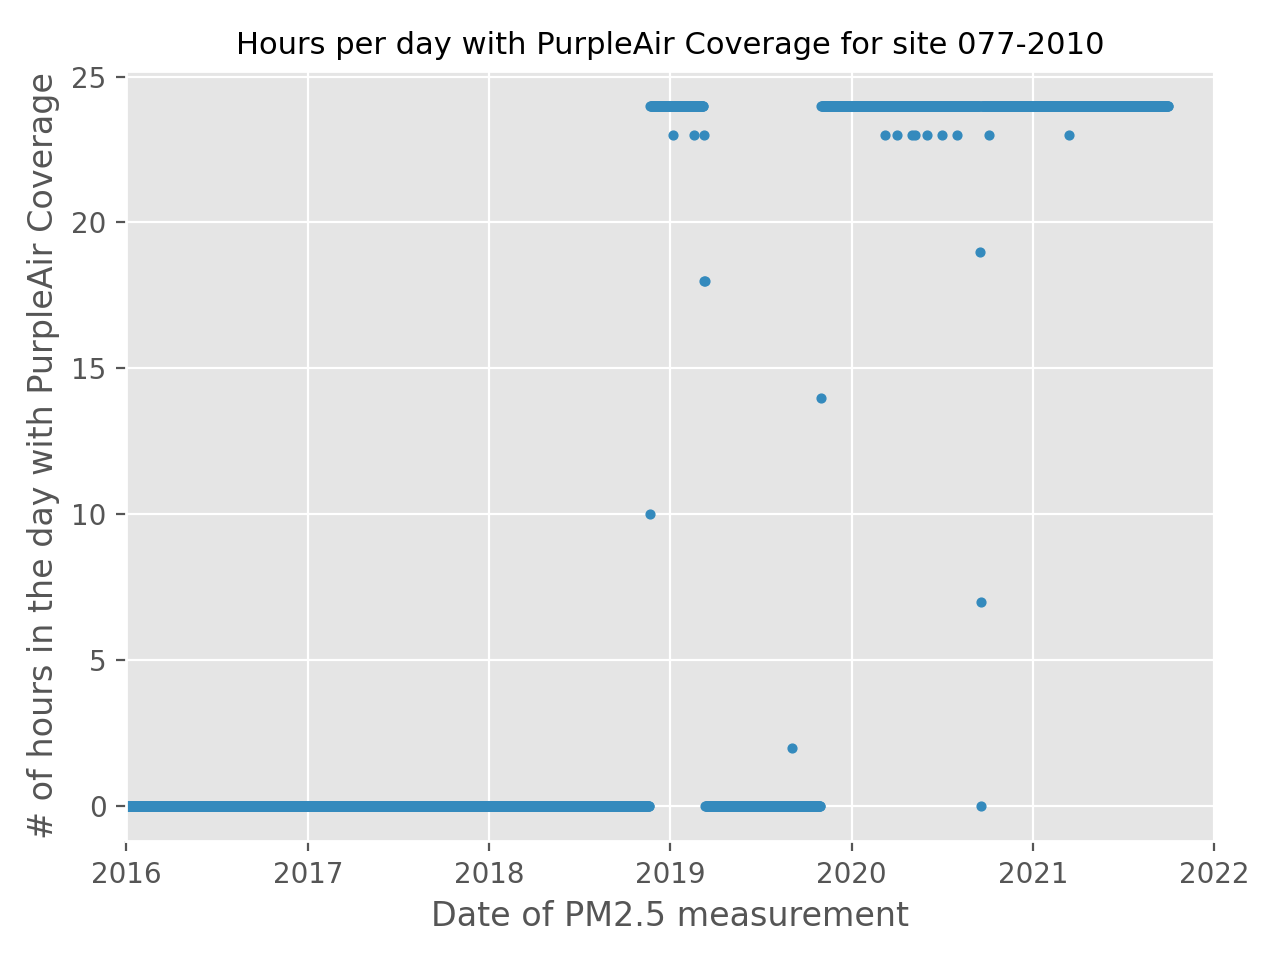
\includegraphics[width=0.8\textwidth]{appendix/site_plots/site-077-2010_pa-daily-covereage.png}
\caption{Scatter plot indicating the number of hours in each day that this NAAQS monitor has PurpleAir coverage. An hour has PurpleAir coverage if there are any PurpleAir sensor readings within the 5-mile radius of the monitor site for that hour. The weighted average is calculated for that hour using all the available PurpleAir readings within 5 miles. This monitor is at site 2010 in county 077 (FIPS code).}
\label{fig:hourly_coverage_077-2010}
\end{figure}
\begin{figure}
\centering
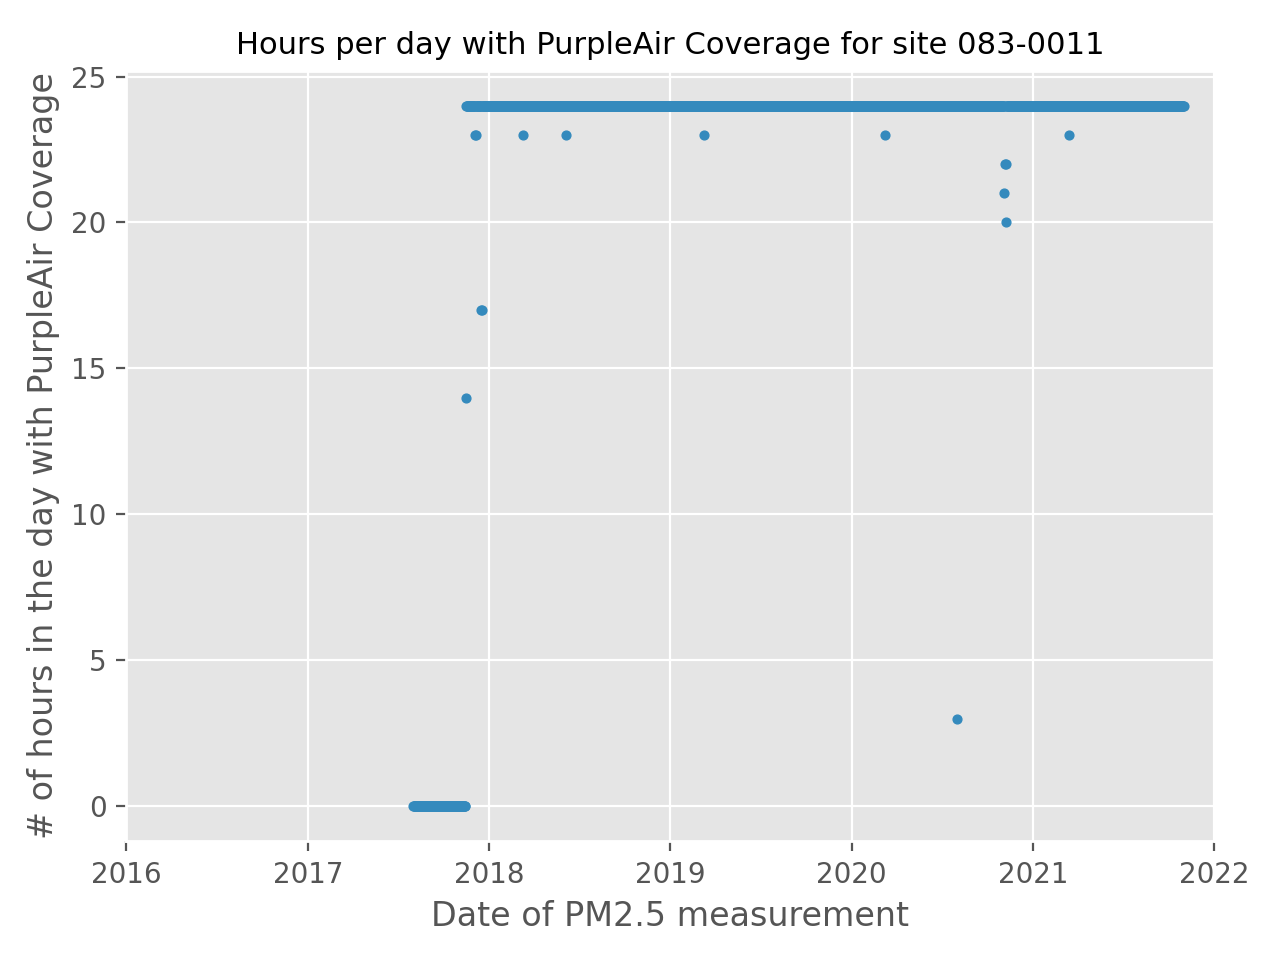
\includegraphics[width=0.8\textwidth]{appendix/site_plots/site-083-0011_pa-daily-covereage.png}
\caption{Scatter plot indicating the number of hours in each day that this NAAQS monitor has PurpleAir coverage. An hour has PurpleAir coverage if there are any PurpleAir sensor readings within the 5-mile radius of the monitor site for that hour. The weighted average is calculated for that hour using all the available PurpleAir readings within 5 miles. This monitor is at site 0011 in county 083 (FIPS code).}
\label{fig:hourly_coverage_083-0011}
\end{figure}
\begin{figure}
\centering
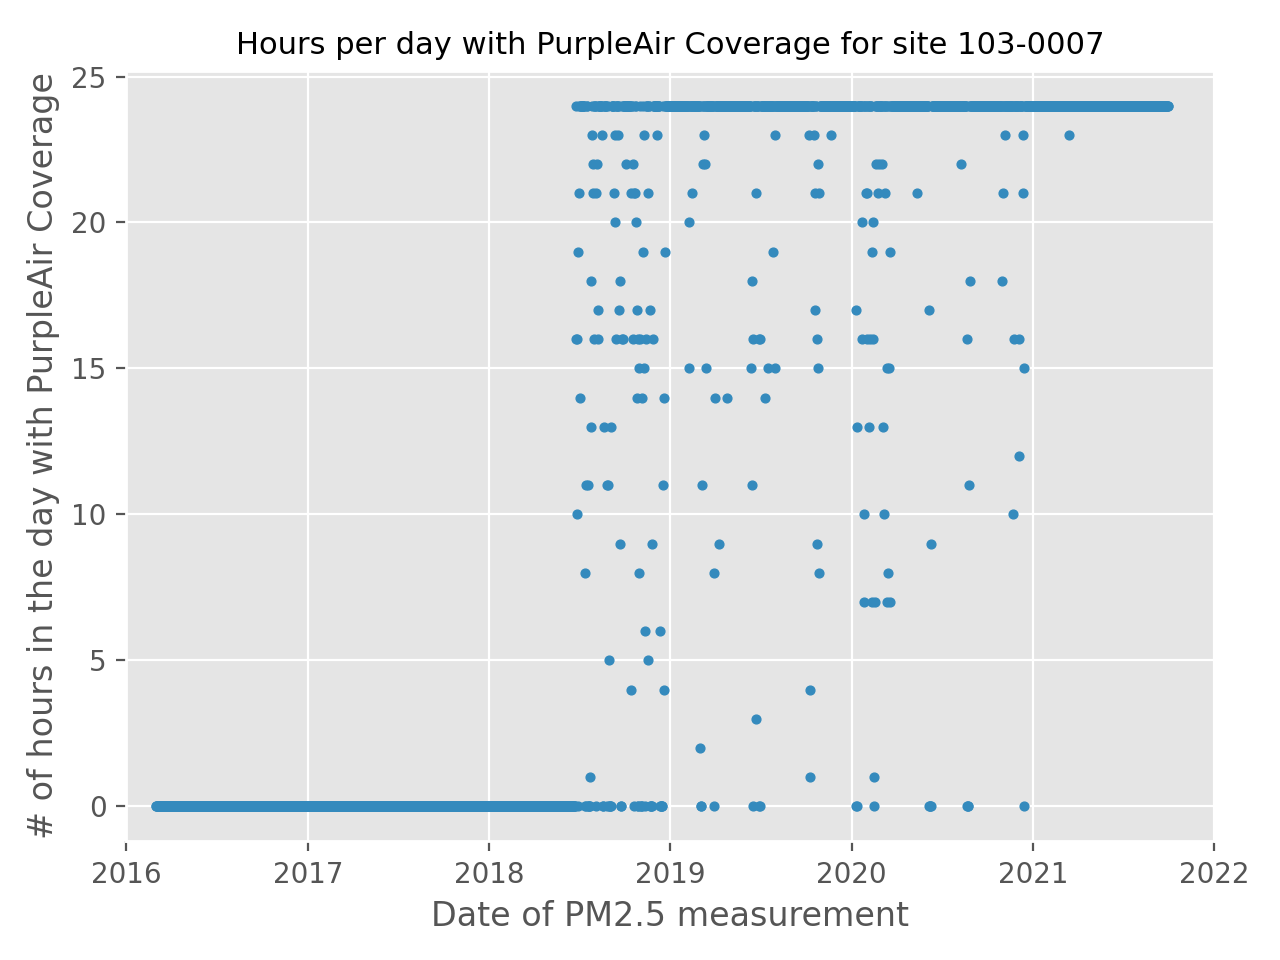
\includegraphics[width=0.8\textwidth]{appendix/site_plots/site-103-0007_pa-daily-covereage.png}
\caption{Scatter plot indicating the number of hours in each day that this NAAQS monitor has PurpleAir coverage. An hour has PurpleAir coverage if there are any PurpleAir sensor readings within the 5-mile radius of the monitor site for that hour. The weighted average is calculated for that hour using all the available PurpleAir readings within 5 miles. This monitor is at site 0007 in county 103 (FIPS code).}
\label{fig:hourly_coverage_103-0007}
\end{figure}
%=========================================
%  PurpleAir EPA Non-missing Comparison
%=========================================
\begin{figure}
\centering
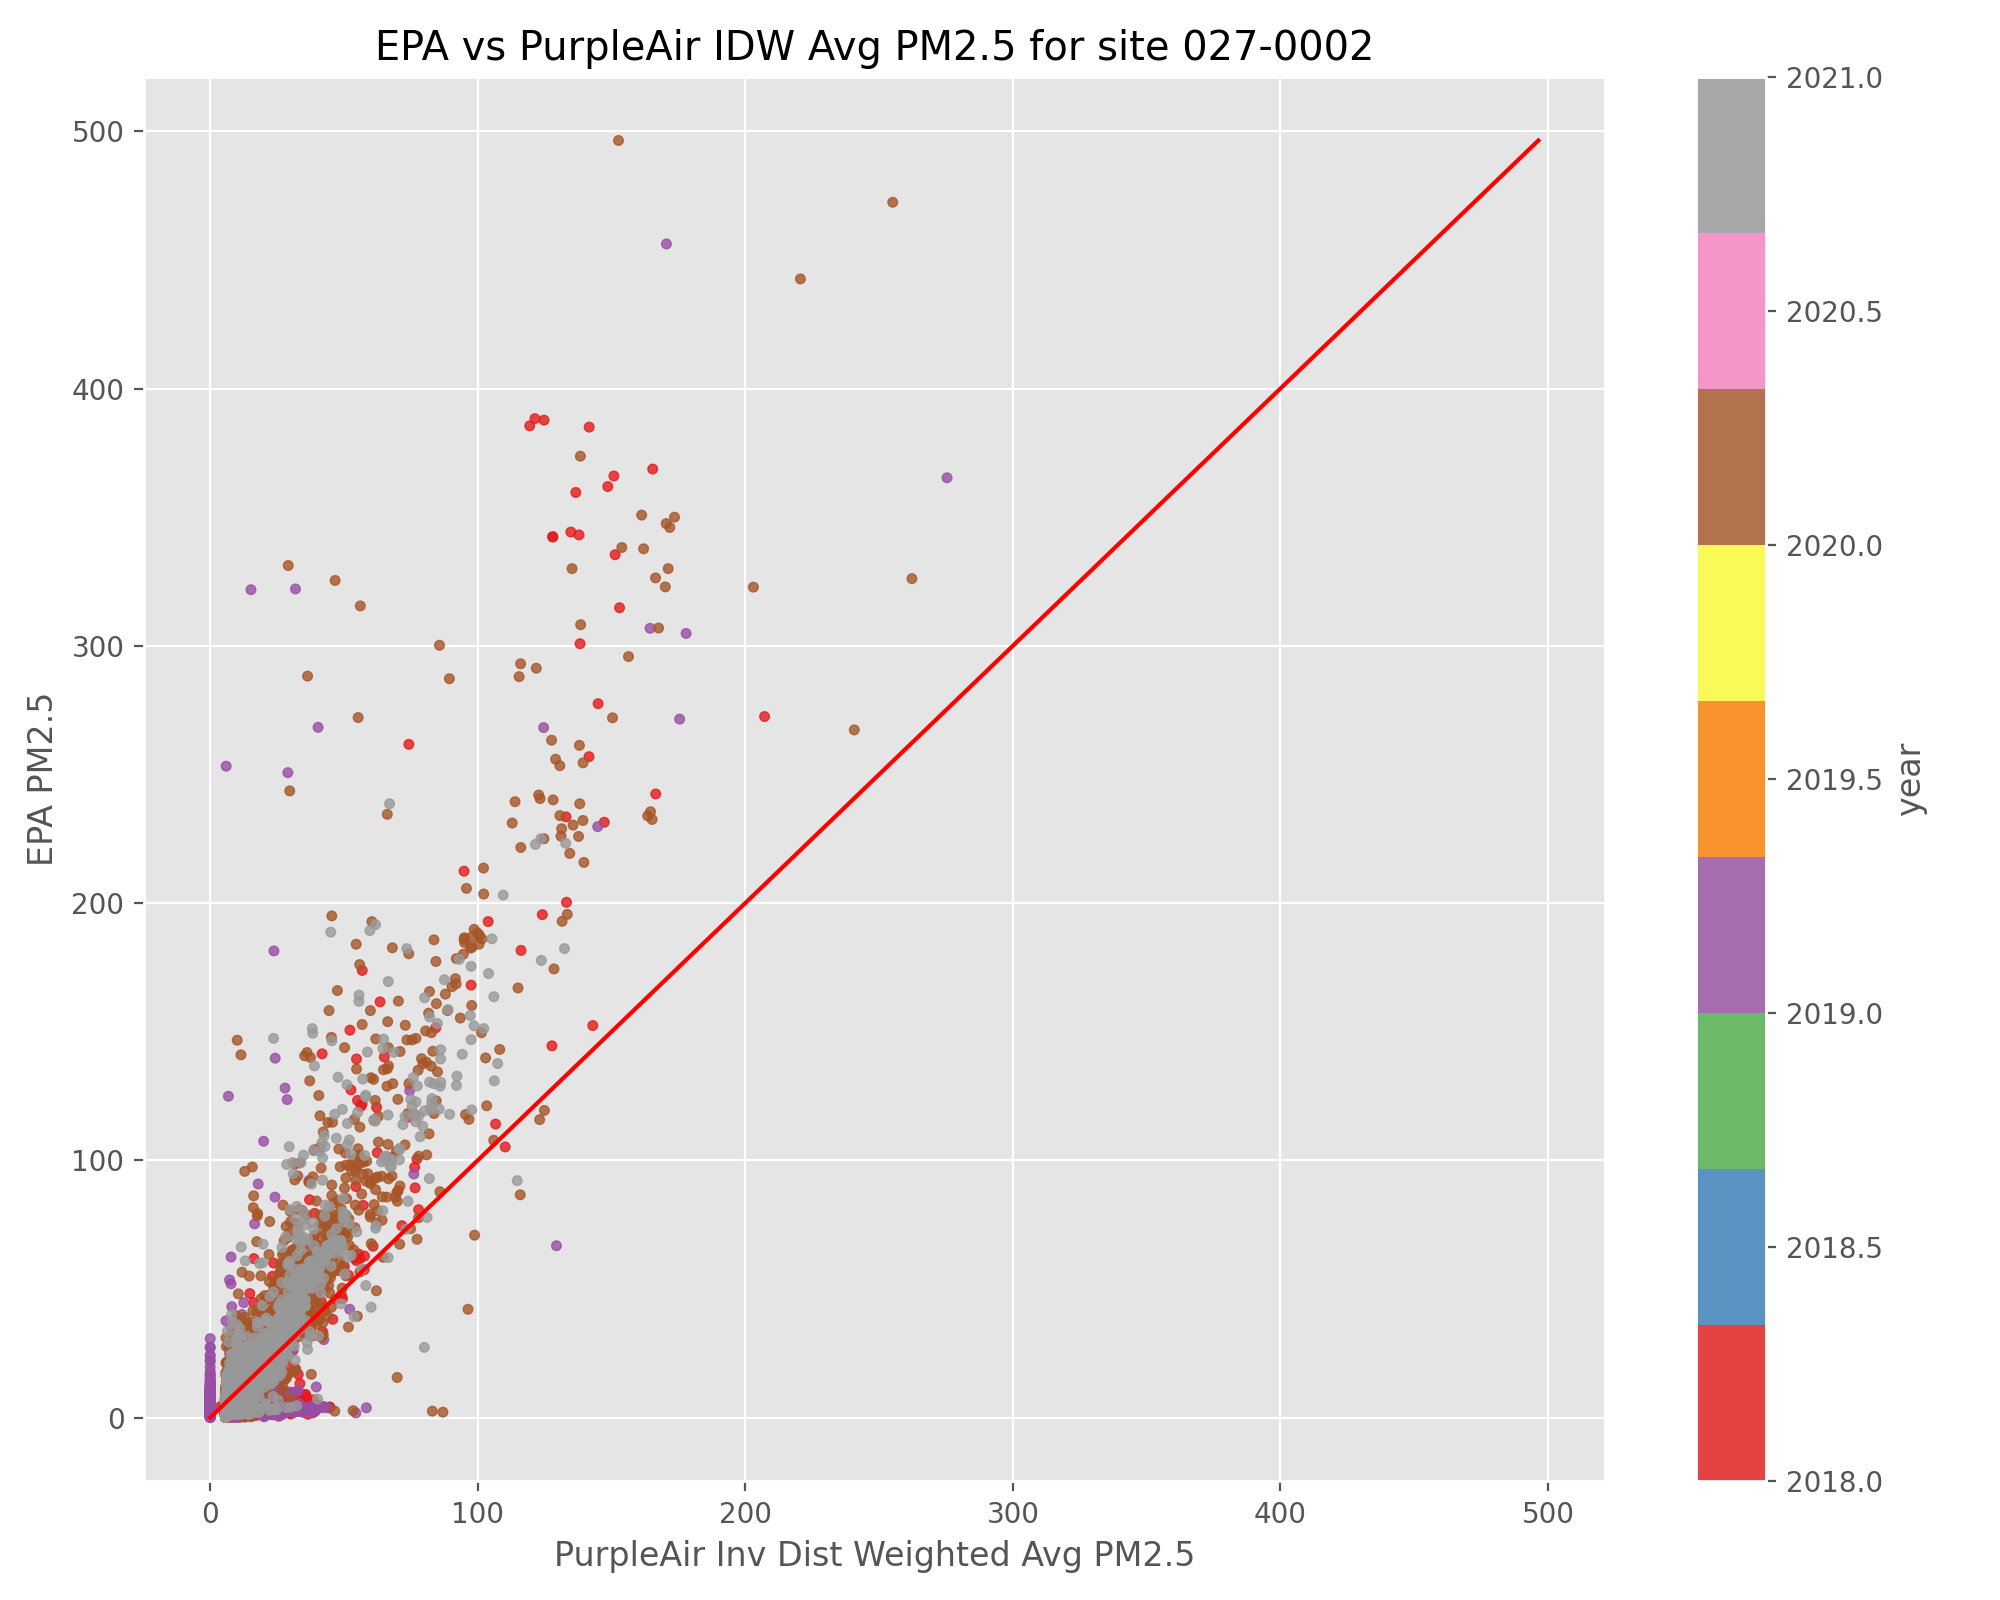
\includegraphics[width=0.8\textwidth]{appendix/site_plots/site-027-0002_epa-pa-hourly-plot.png}
\caption{Scatter plot comparing reported hourly PM2.5 measurements: the x-axis represents the IDW-weighted average of PurpleAir measurements, the y-axis represents reported NAAQS-primary monitor measurements. The red line is a 45$^\circ$ line, representing perfect correlation between the PurpleAir average and the NAAQS-primary monitor. This monitor is at site 0002 in county 027 (FIPS code).}
\label{fig:pa-epa-compare_027-0002}
\end{figure}
\begin{figure}
\centering
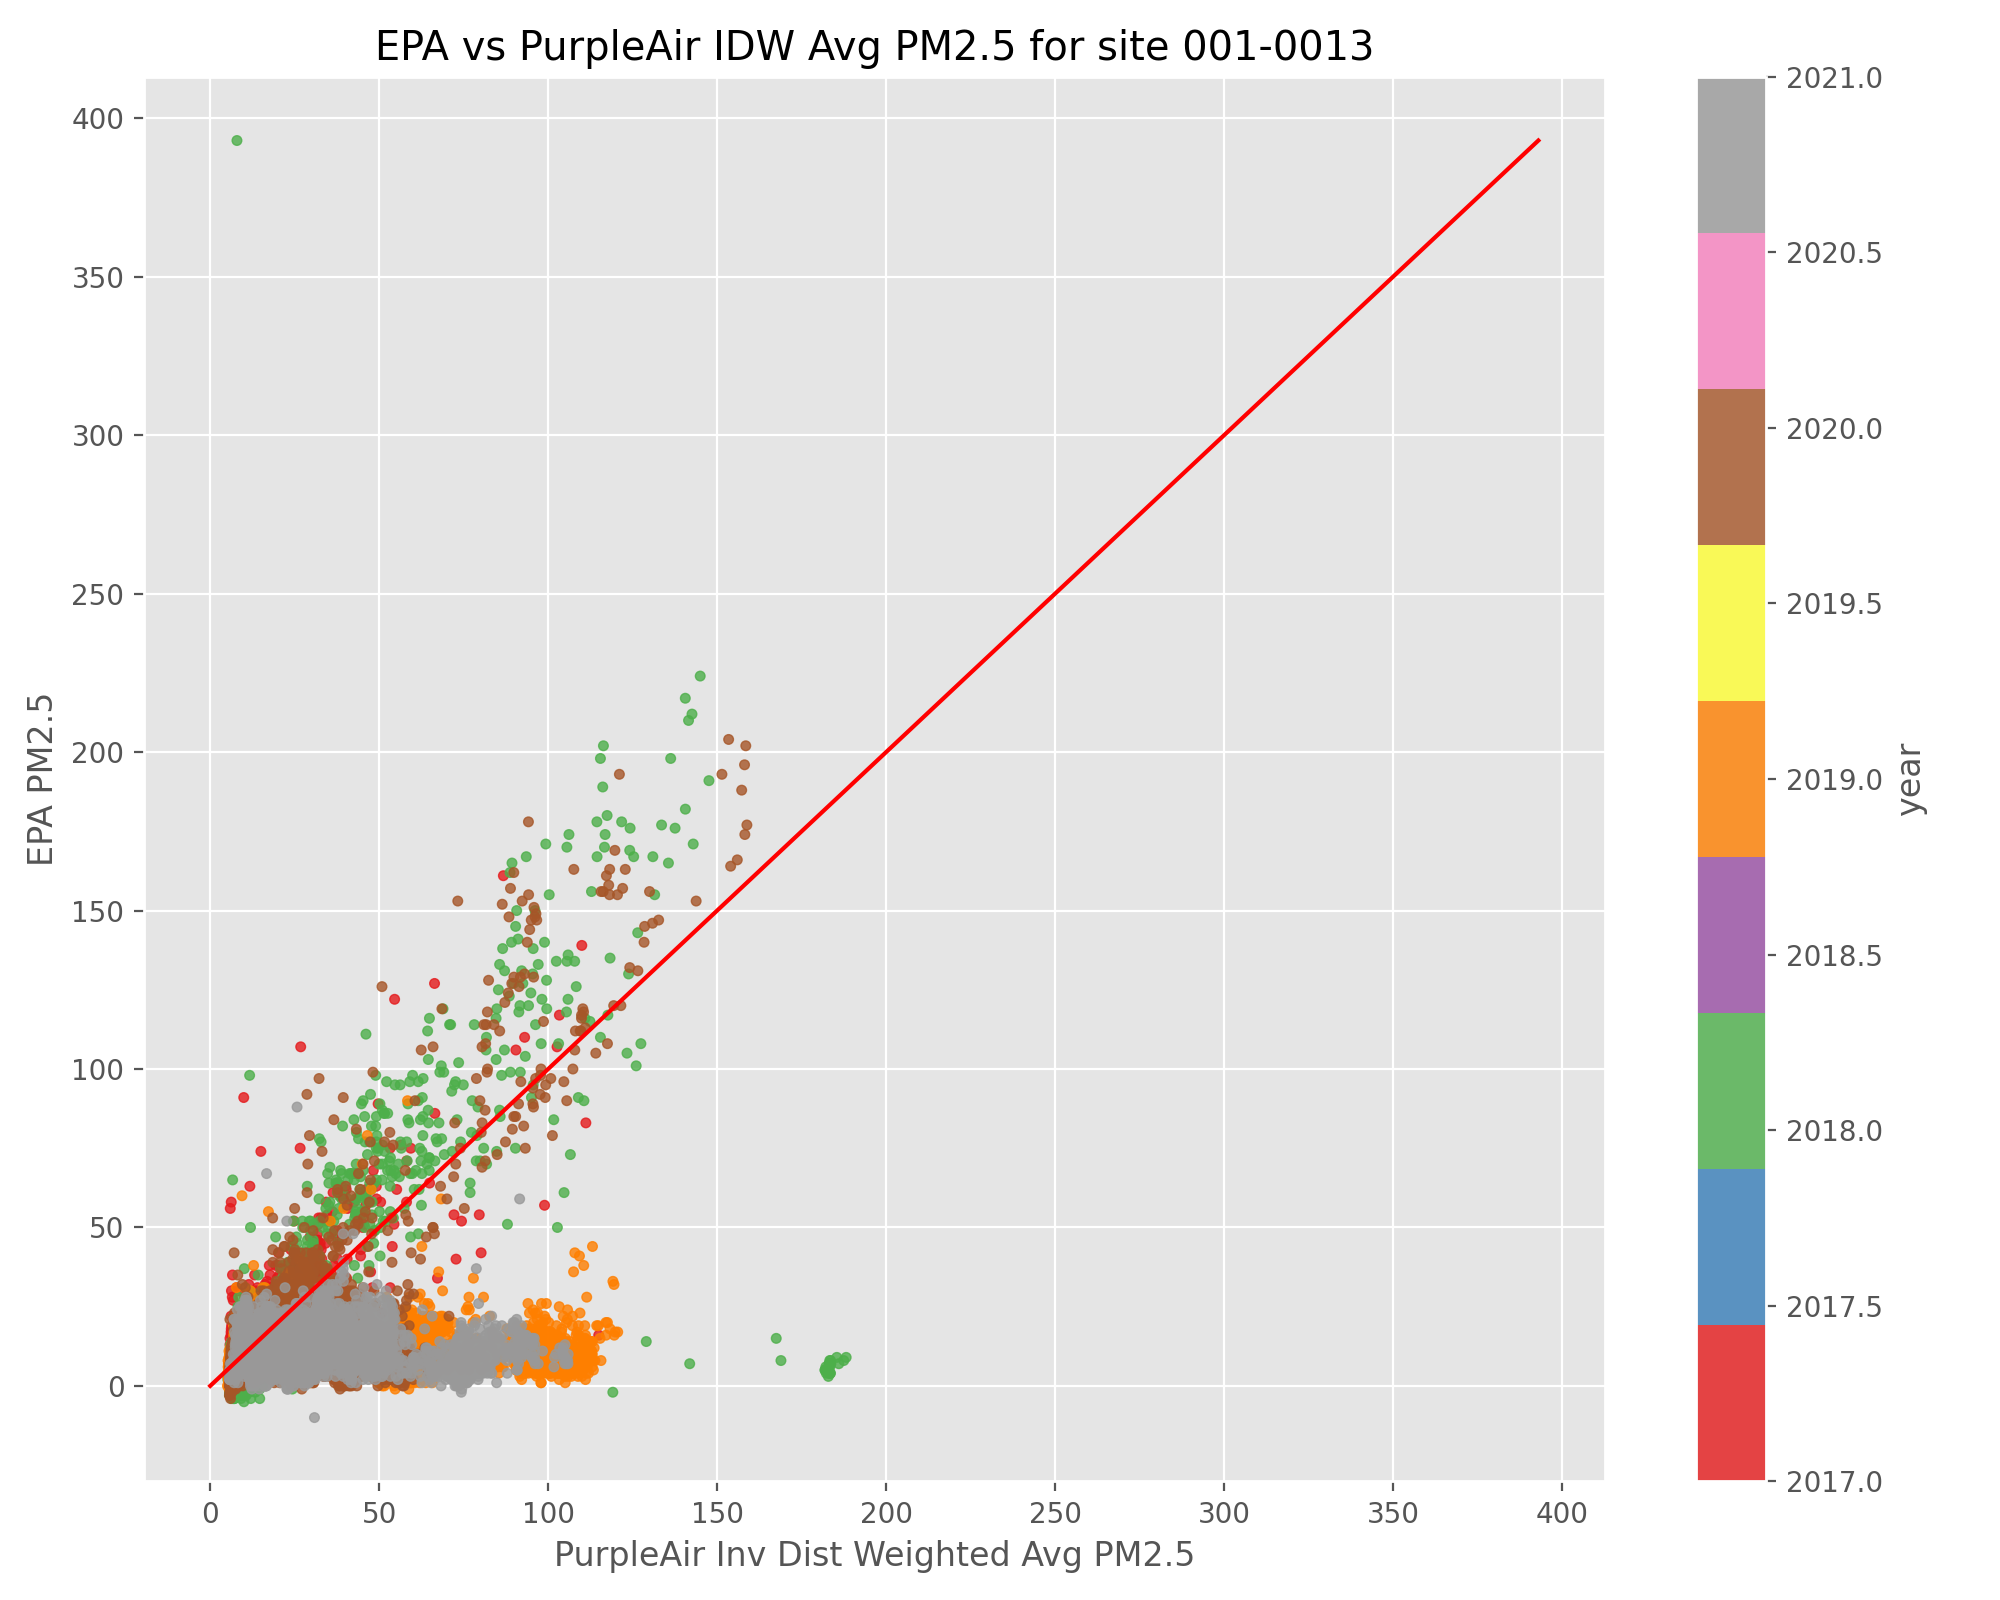
\includegraphics[width=0.8\textwidth]{appendix/site_plots/site-001-0013_epa-pa-hourly-plot.png}
\caption{Scatter plot comparing reported hourly PM2.5 measurements: the x-axis represents the IDW-weighted average of PurpleAir measurements, the y-axis represents reported NAAQS-primary monitor measurements. The red line is a 45$^\circ$ line, representing perfect correlation between the PurpleAir average and the NAAQS-primary monitor. This monitor is at site 0013 in county 001 (FIPS code).}
\label{fig:pa-epa-compare_001-0013}
\end{figure}
\begin{figure}
\centering
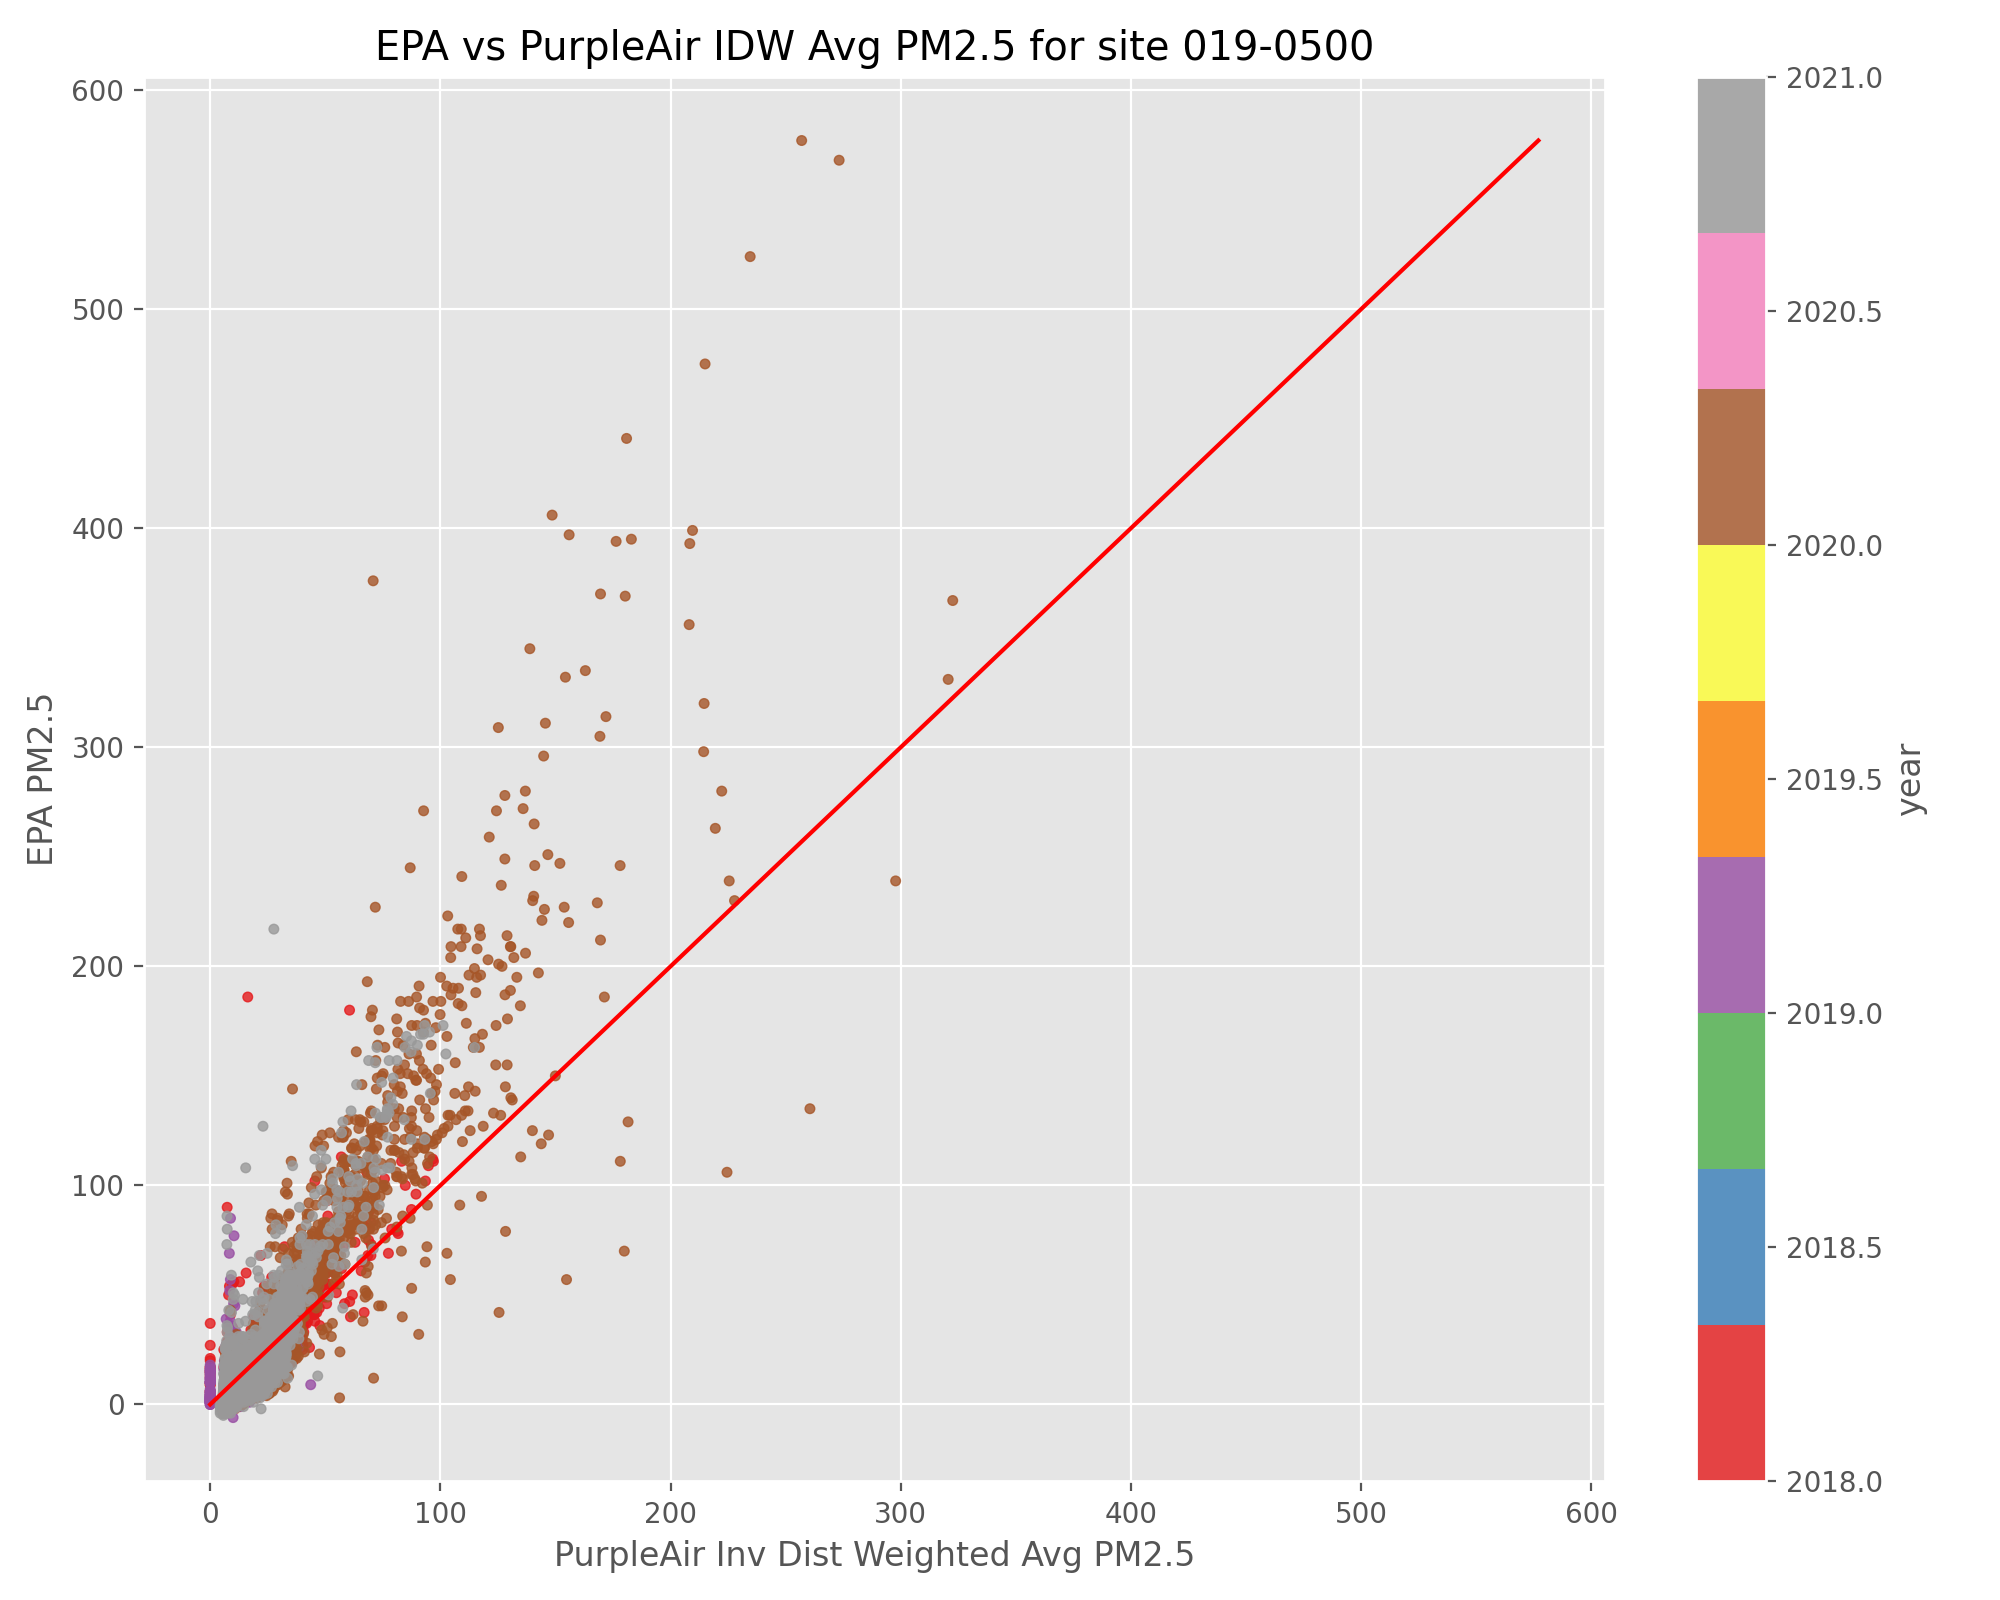
\includegraphics[width=0.8\textwidth]{appendix/site_plots/site-019-0500_epa-pa-hourly-plot.png}
\caption{Scatter plot comparing reported hourly PM2.5 measurements: the x-axis represents the IDW-weighted average of PurpleAir measurements, the y-axis represents reported NAAQS-primary monitor measurements. The red line is a 45$^\circ$ line, representing perfect correlation between the PurpleAir average and the NAAQS-primary monitor. This monitor is at site 0500 in county 019 (FIPS code).}
\label{fig:pa-epa-compare_019-0500}
\end{figure}
\begin{figure}
\centering
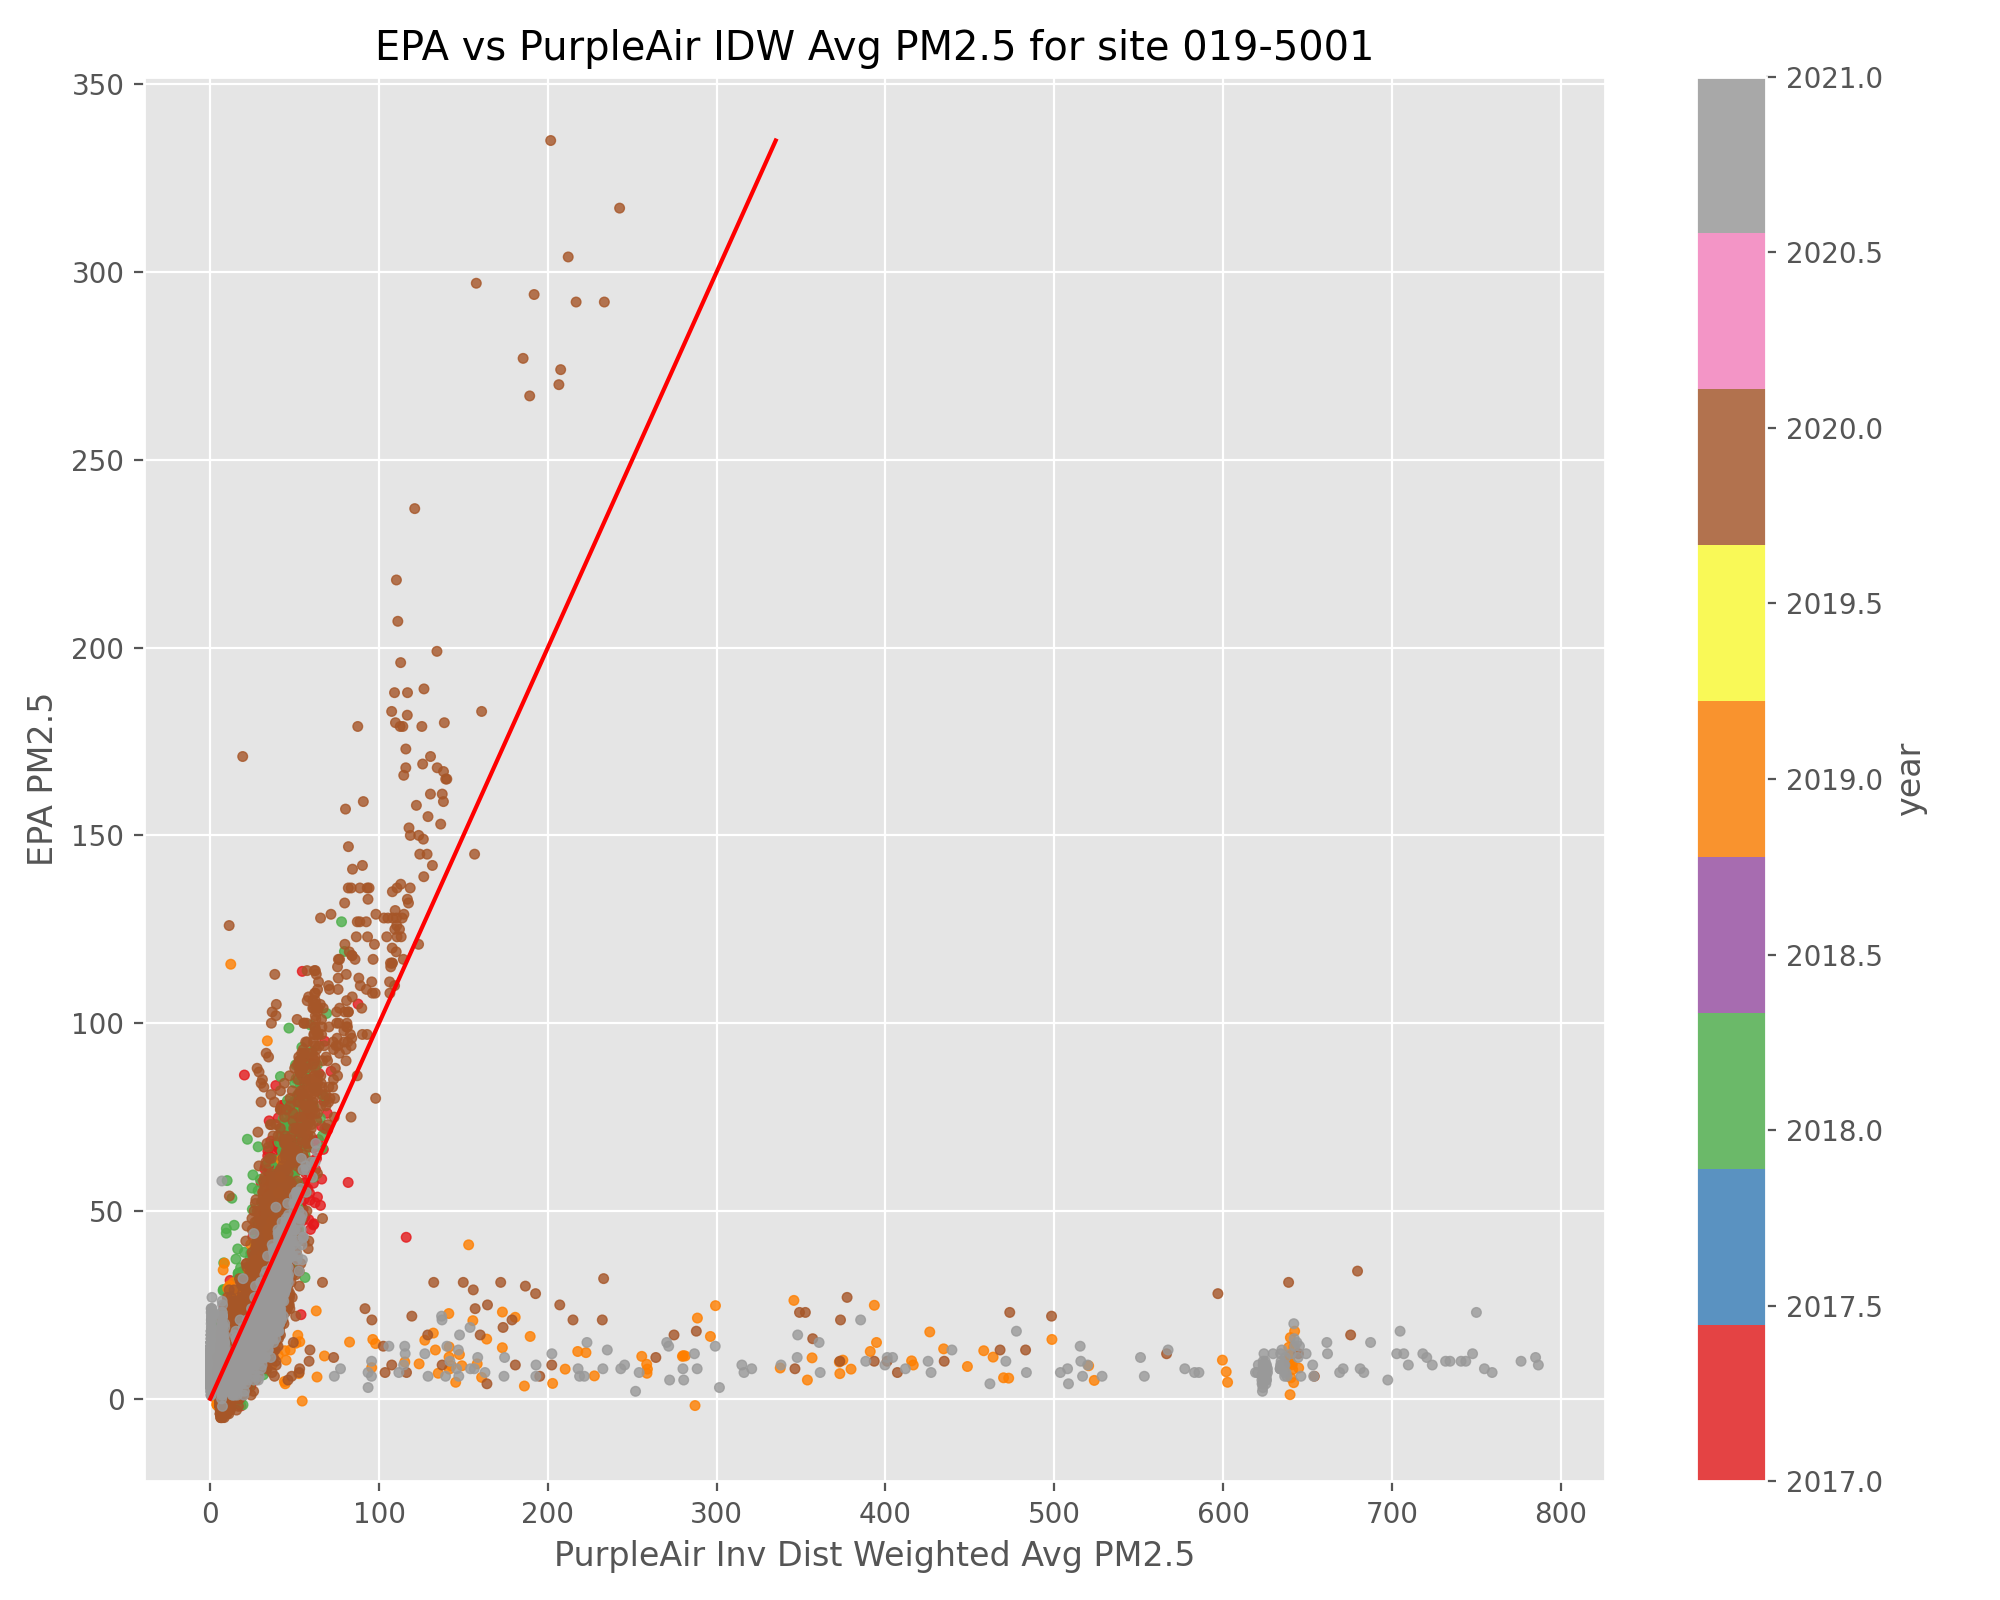
\includegraphics[width=0.8\textwidth]{appendix/site_plots/site-019-5001_epa-pa-hourly-plot.png}
\caption{Scatter plot comparing reported hourly PM2.5 measurements: the x-axis represents the IDW-weighted average of PurpleAir measurements, the y-axis represents reported NAAQS-primary monitor measurements. The red line is a 45$^\circ$ line, representing perfect correlation between the PurpleAir average and the NAAQS-primary monitor. This monitor is at site 5001 in county 019 (FIPS code).}
\label{fig:pa-epa-compare_019-5001}
\end{figure}
\begin{figure}
\centering
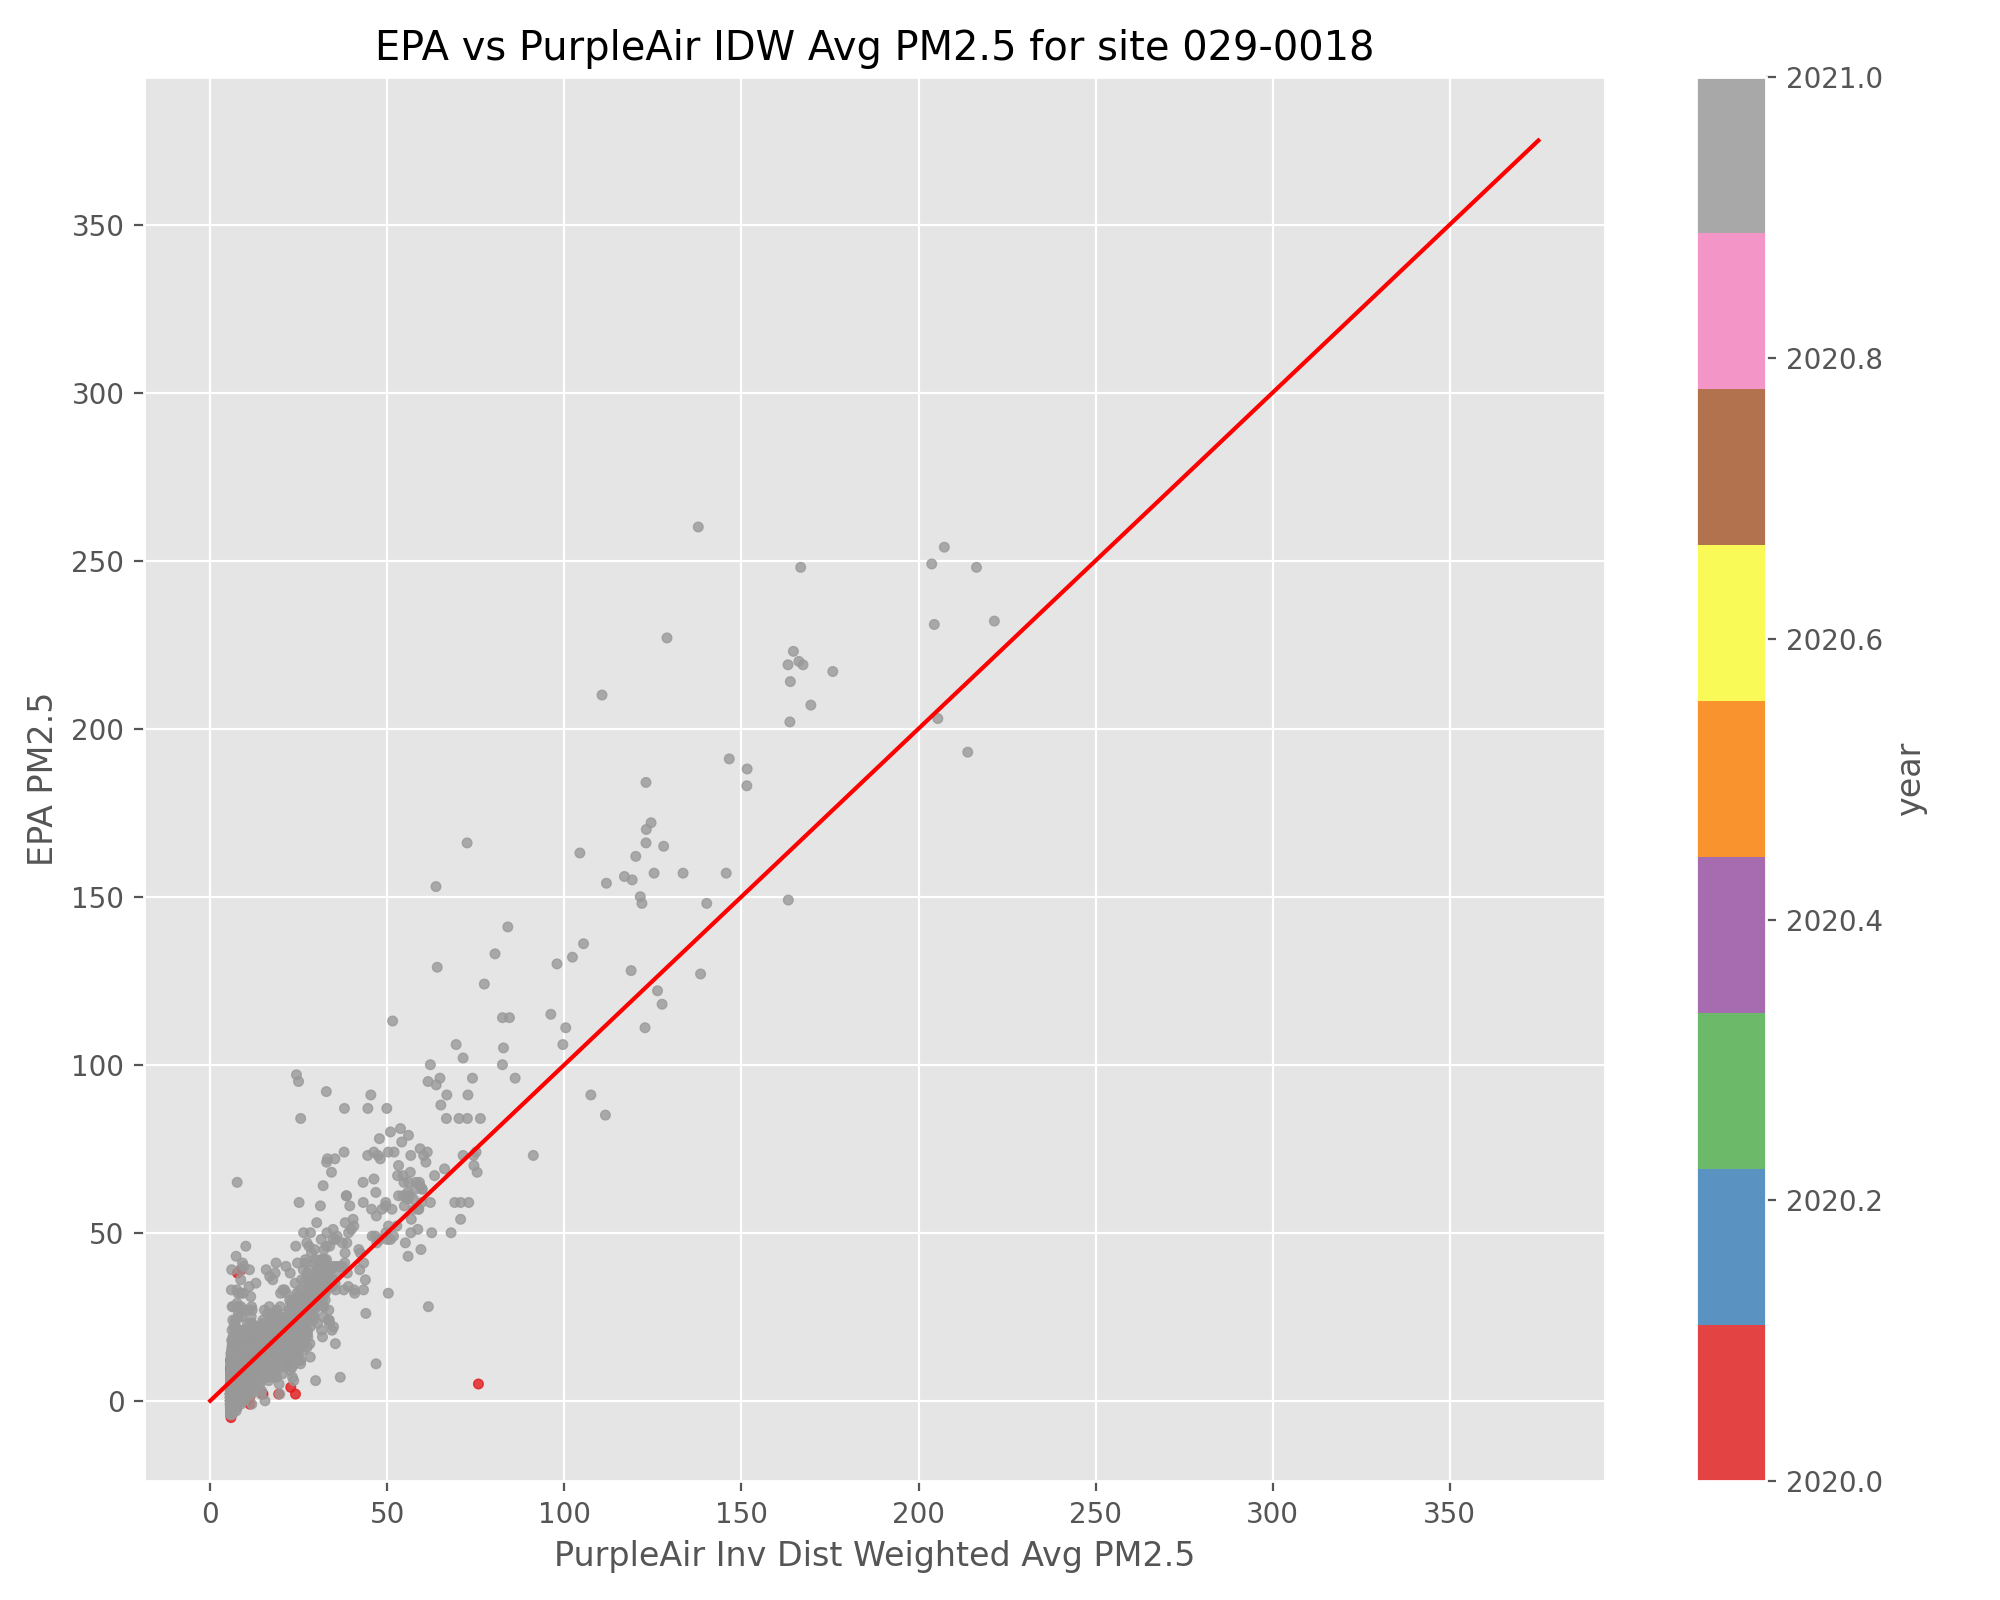
\includegraphics[width=0.8\textwidth]{appendix/site_plots/site-029-0018_epa-pa-hourly-plot.png}
\caption{Scatter plot comparing reported hourly PM2.5 measurements: the x-axis represents the IDW-weighted average of PurpleAir measurements, the y-axis represents reported NAAQS-primary monitor measurements. The red line is a 45$^\circ$ line, representing perfect correlation between the PurpleAir average and the NAAQS-primary monitor. This monitor is at site 0018 in county 029 (FIPS code).}
\label{fig:pa-epa-compare_029-0018}
\end{figure}
\begin{figure}
\centering
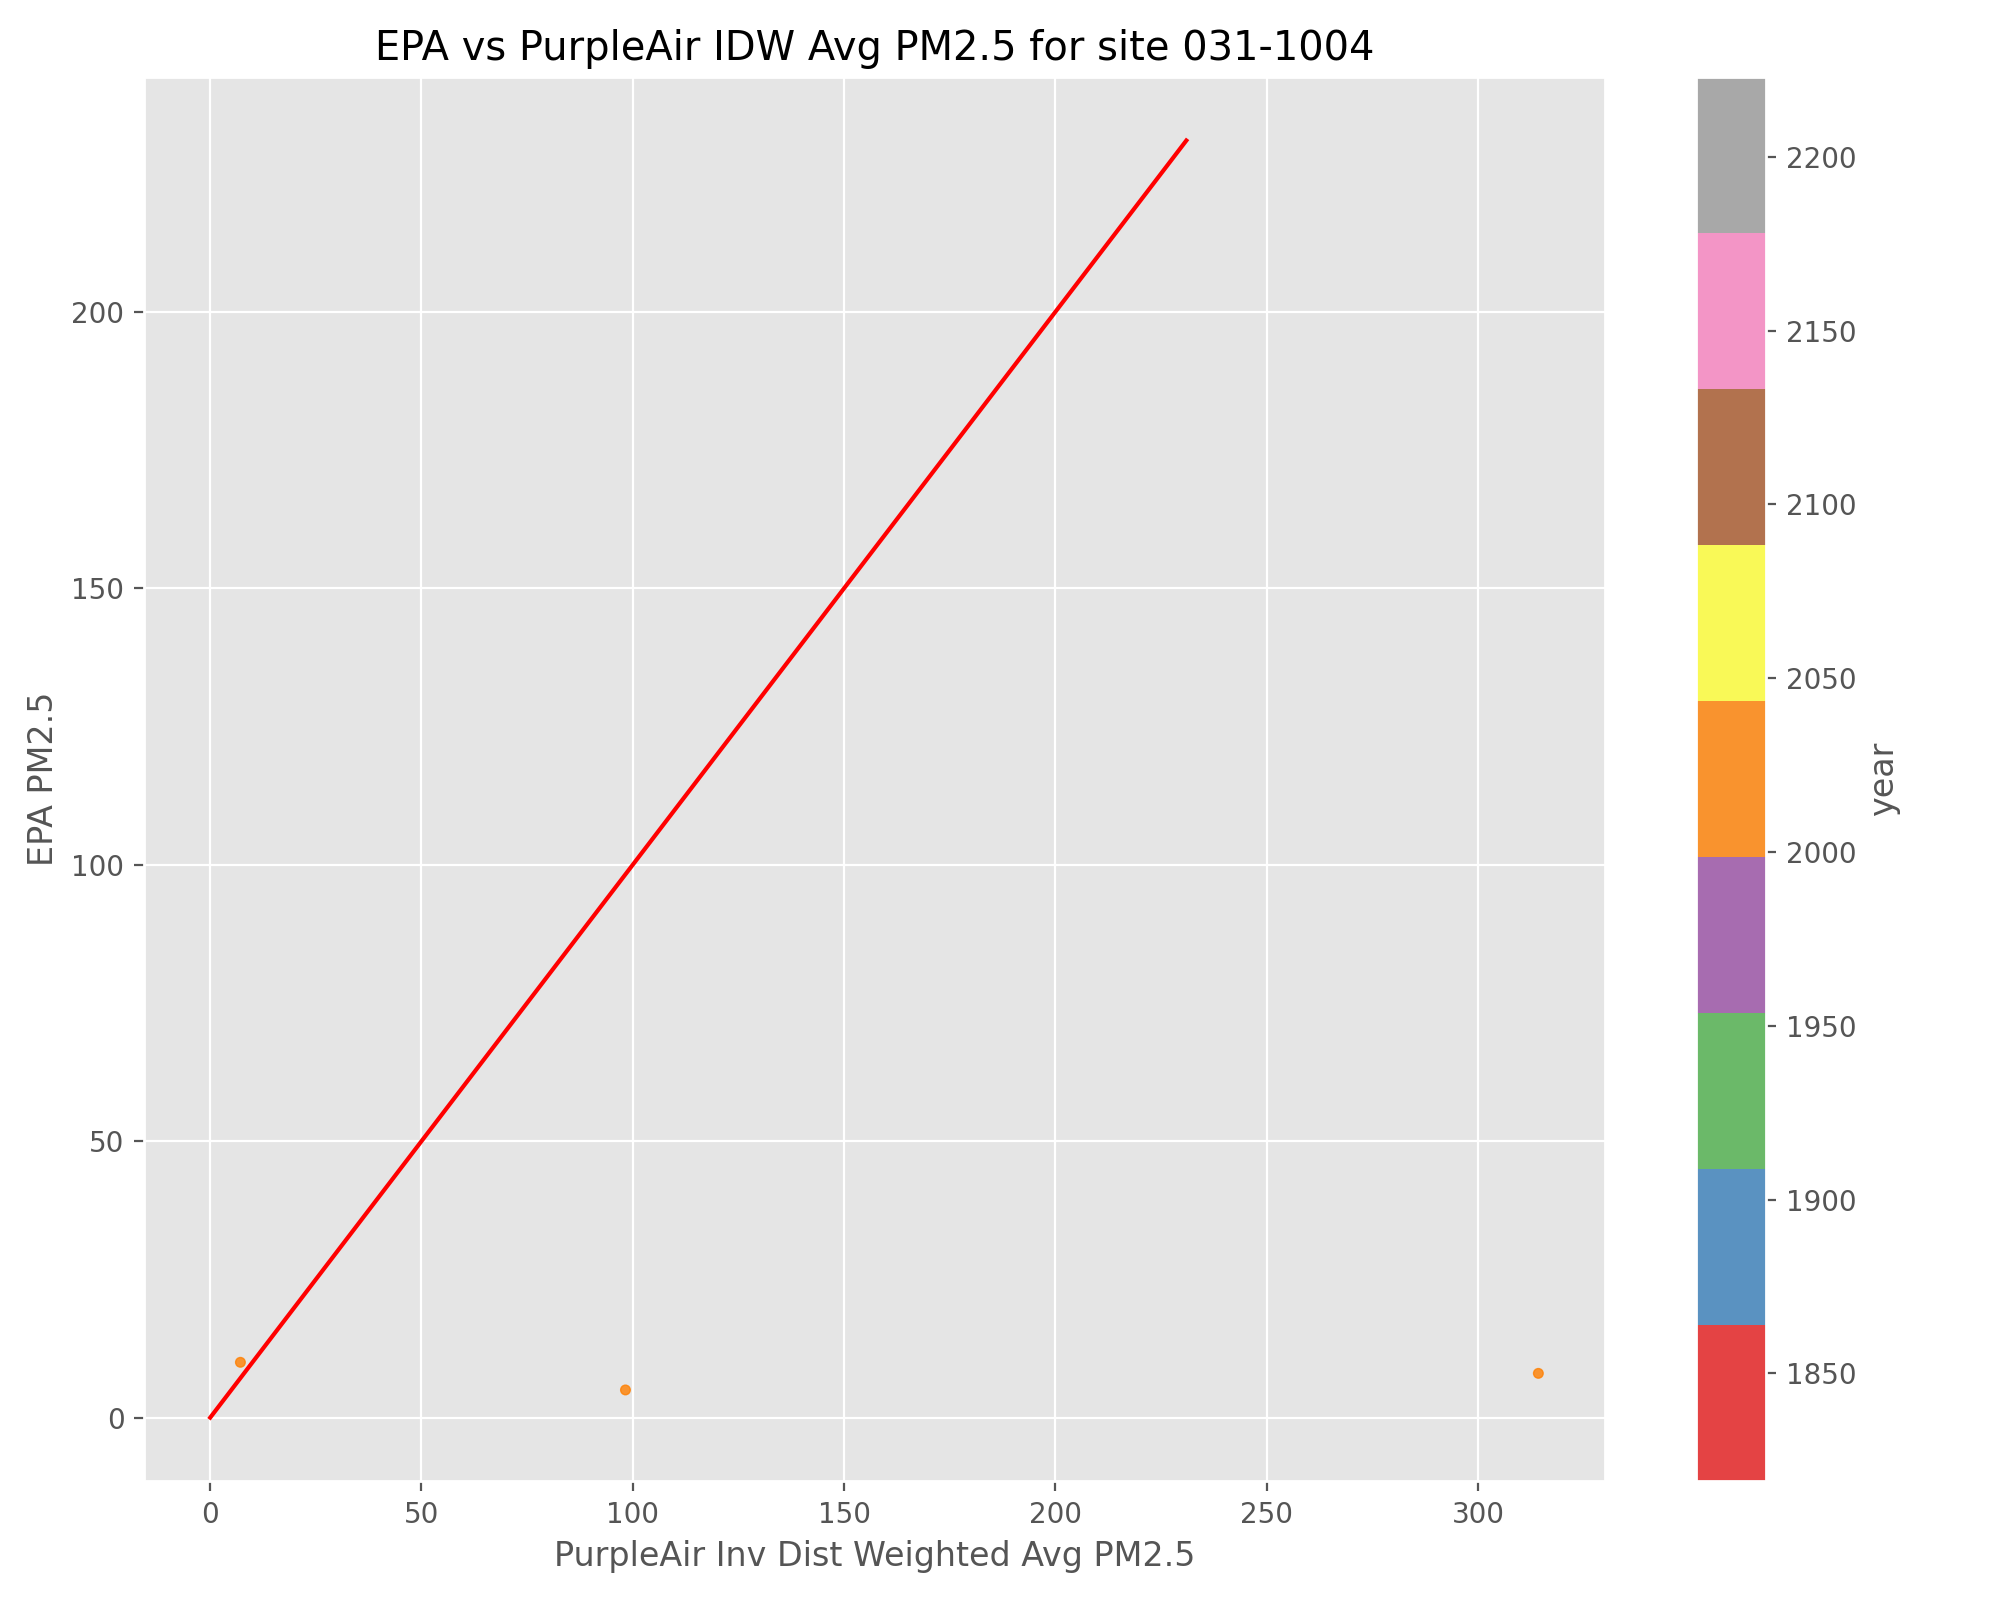
\includegraphics[width=0.8\textwidth]{appendix/site_plots/site-031-1004_epa-pa-hourly-plot.png}
\caption{Scatter plot comparing reported hourly PM2.5 measurements: the x-axis represents the IDW-weighted average of PurpleAir measurements, the y-axis represents reported NAAQS-primary monitor measurements. The red line is a 45$^\circ$ line, representing perfect correlation between the PurpleAir average and the NAAQS-primary monitor. This monitor is at site 1004 in county 031 (FIPS code).}
\label{fig:pa-epa-compare_031-1004}
\end{figure}
\begin{figure}
\centering
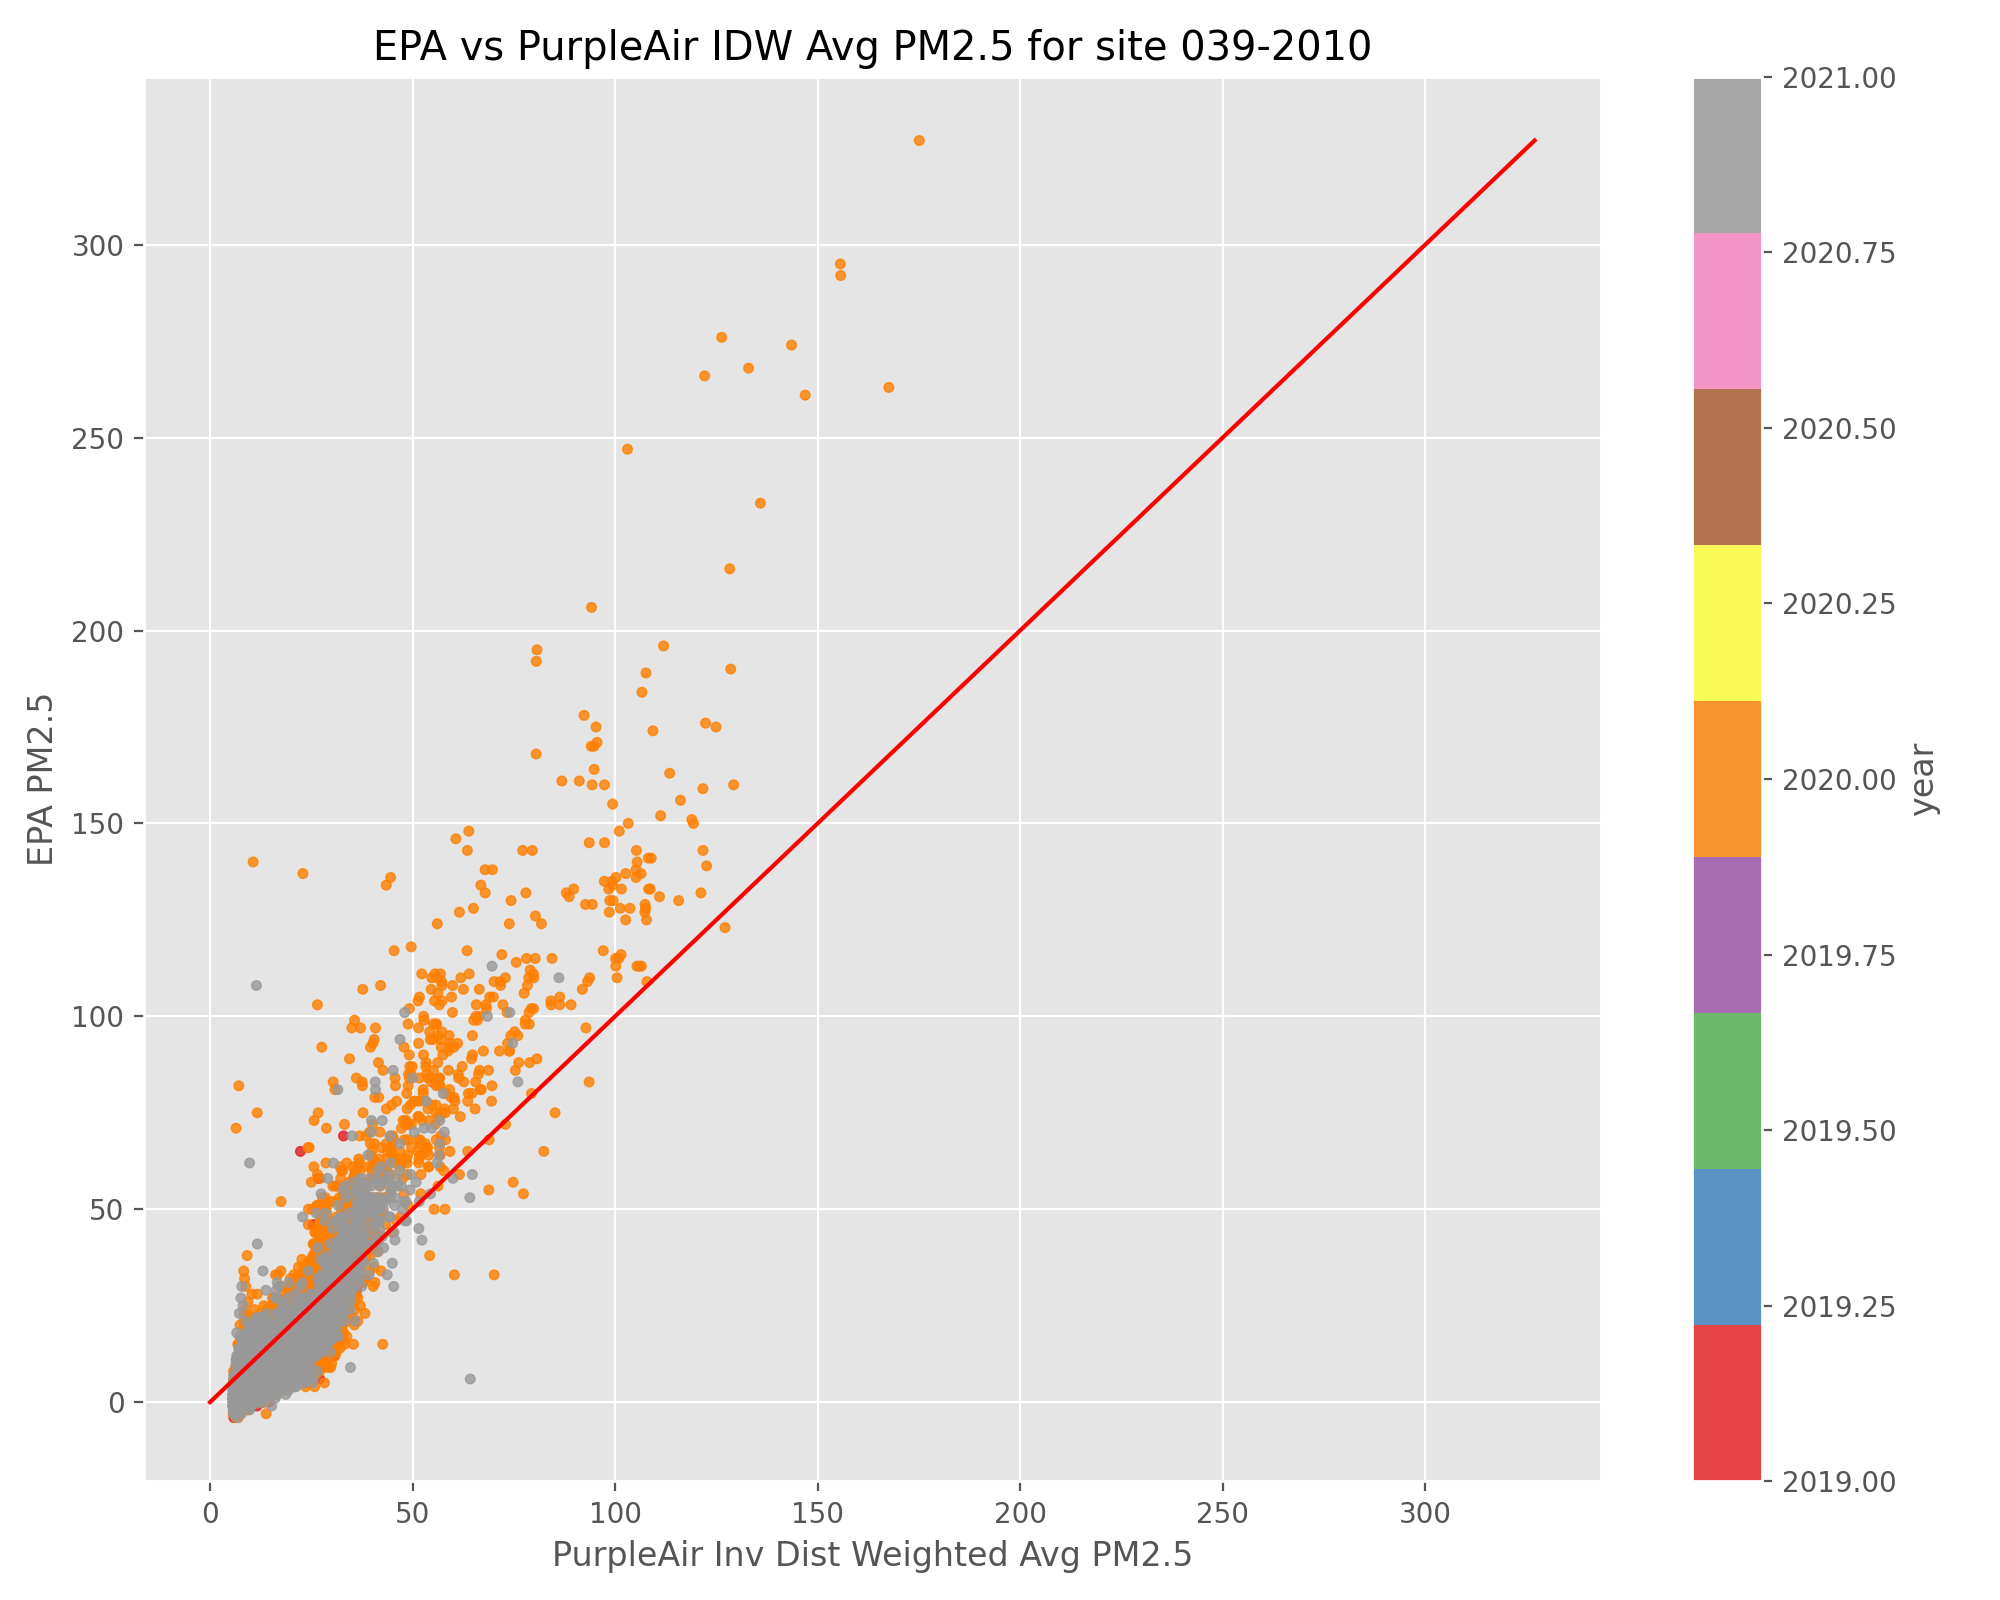
\includegraphics[width=0.8\textwidth]{appendix/site_plots/site-039-2010_epa-pa-hourly-plot.png}
\caption{Scatter plot comparing reported hourly PM2.5 measurements: the x-axis represents the IDW-weighted average of PurpleAir measurements, the y-axis represents reported NAAQS-primary monitor measurements. The red line is a 45$^\circ$ line, representing perfect correlation between the PurpleAir average and the NAAQS-primary monitor. This monitor is at site 2010 in county 039 (FIPS code).}
\label{fig:pa-epa-compare_039-2010}
\end{figure}
\begin{figure}
\centering
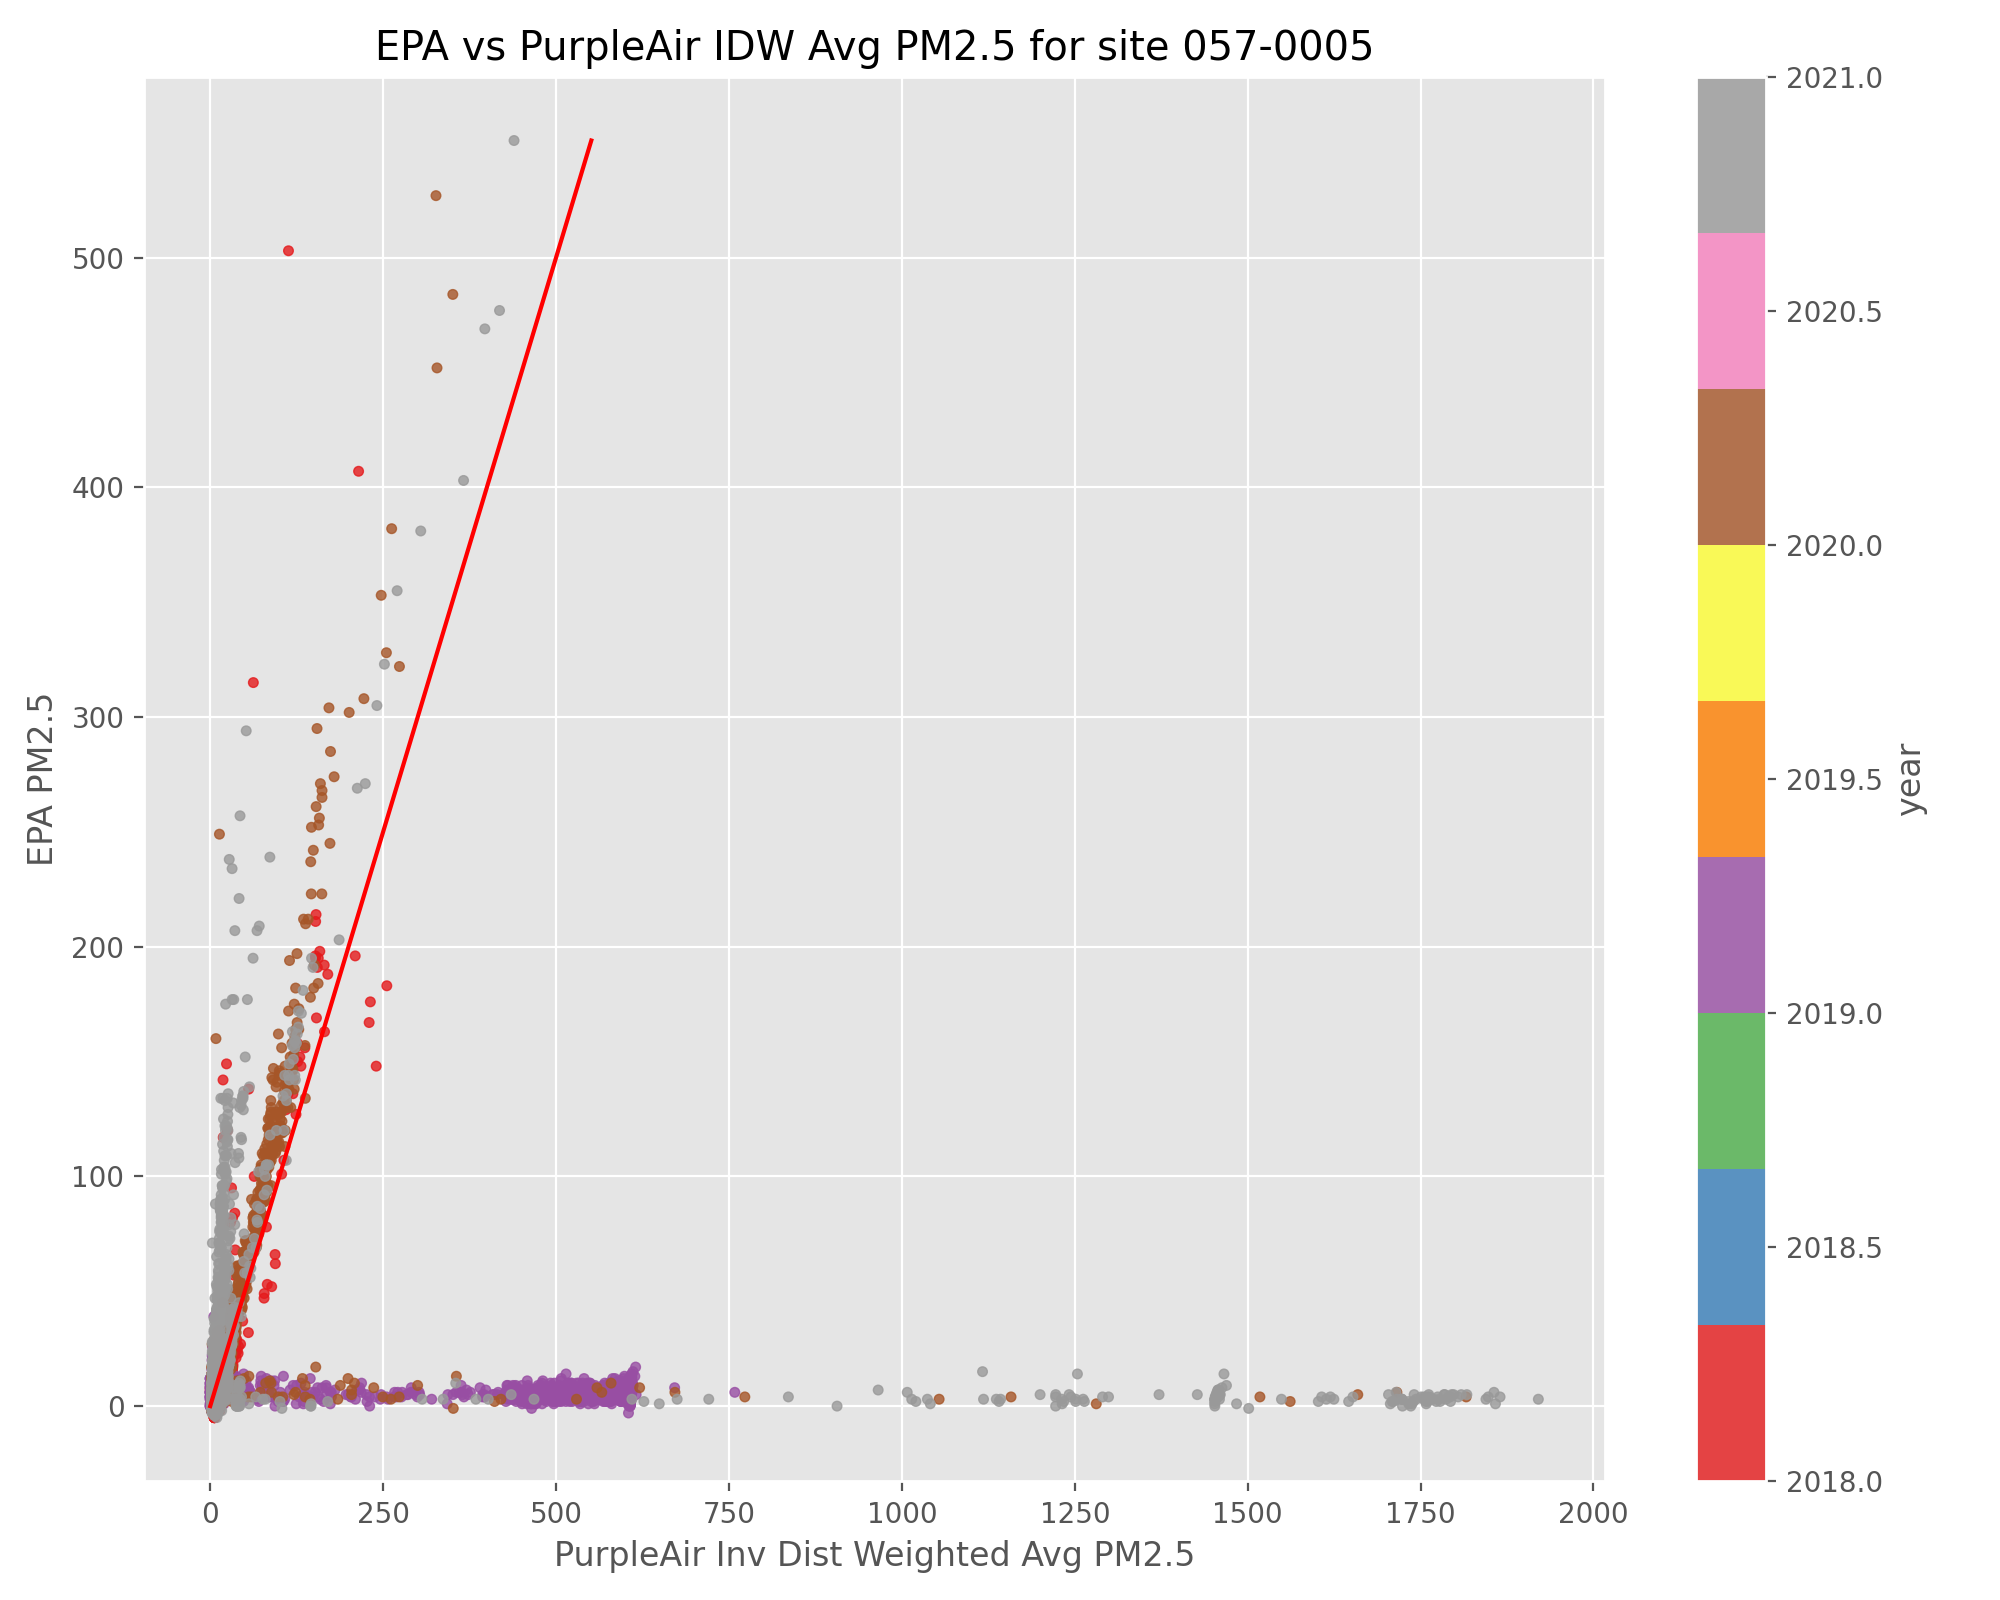
\includegraphics[width=0.8\textwidth]{appendix/site_plots/site-057-0005_epa-pa-hourly-plot.png}
\caption{Scatter plot comparing reported hourly PM2.5 measurements: the x-axis represents the IDW-weighted average of PurpleAir measurements, the y-axis represents reported NAAQS-primary monitor measurements. The red line is a 45$^\circ$ line, representing perfect correlation between the PurpleAir average and the NAAQS-primary monitor. This monitor is at site 0005 in county 057 (FIPS code).}
\label{fig:pa-epa-compare_057-0005}
\end{figure}
\begin{figure}
\centering
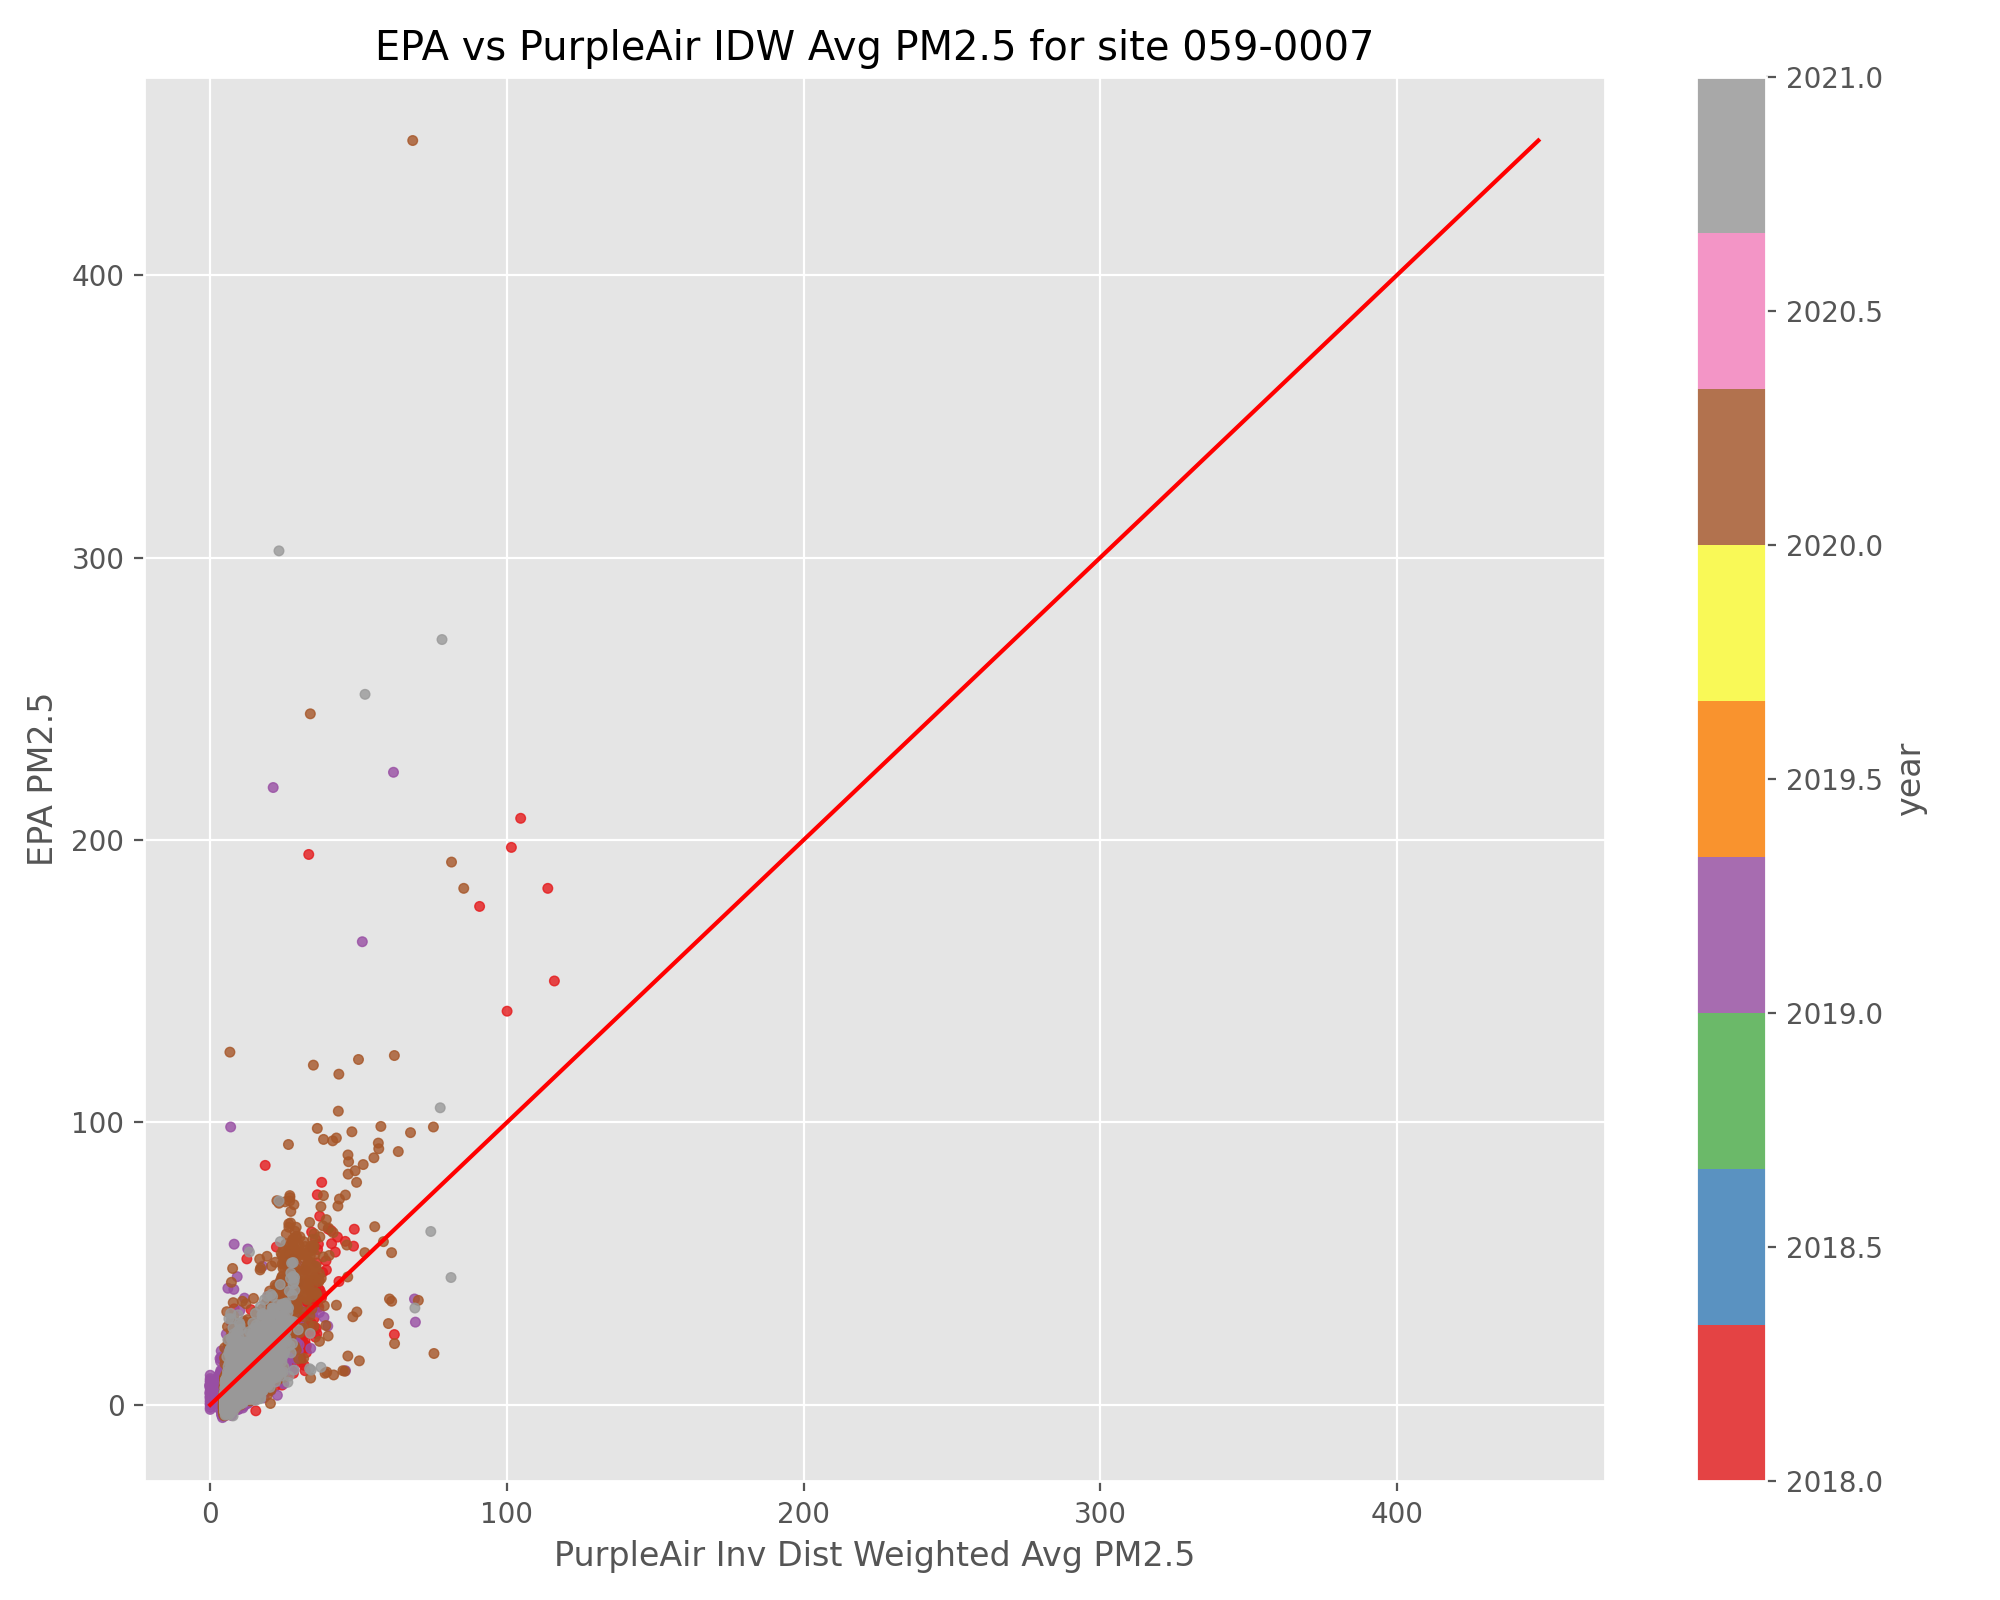
\includegraphics[width=0.8\textwidth]{appendix/site_plots/site-059-0007_epa-pa-hourly-plot.png}
\caption{Scatter plot comparing reported hourly PM2.5 measurements: the x-axis represents the IDW-weighted average of PurpleAir measurements, the y-axis represents reported NAAQS-primary monitor measurements. The red line is a 45$^\circ$ line, representing perfect correlation between the PurpleAir average and the NAAQS-primary monitor. This monitor is at site 0007 in county 059 (FIPS code).}
\label{fig:pa-epa-compare_059-0007}
\end{figure}
\begin{figure}
\centering
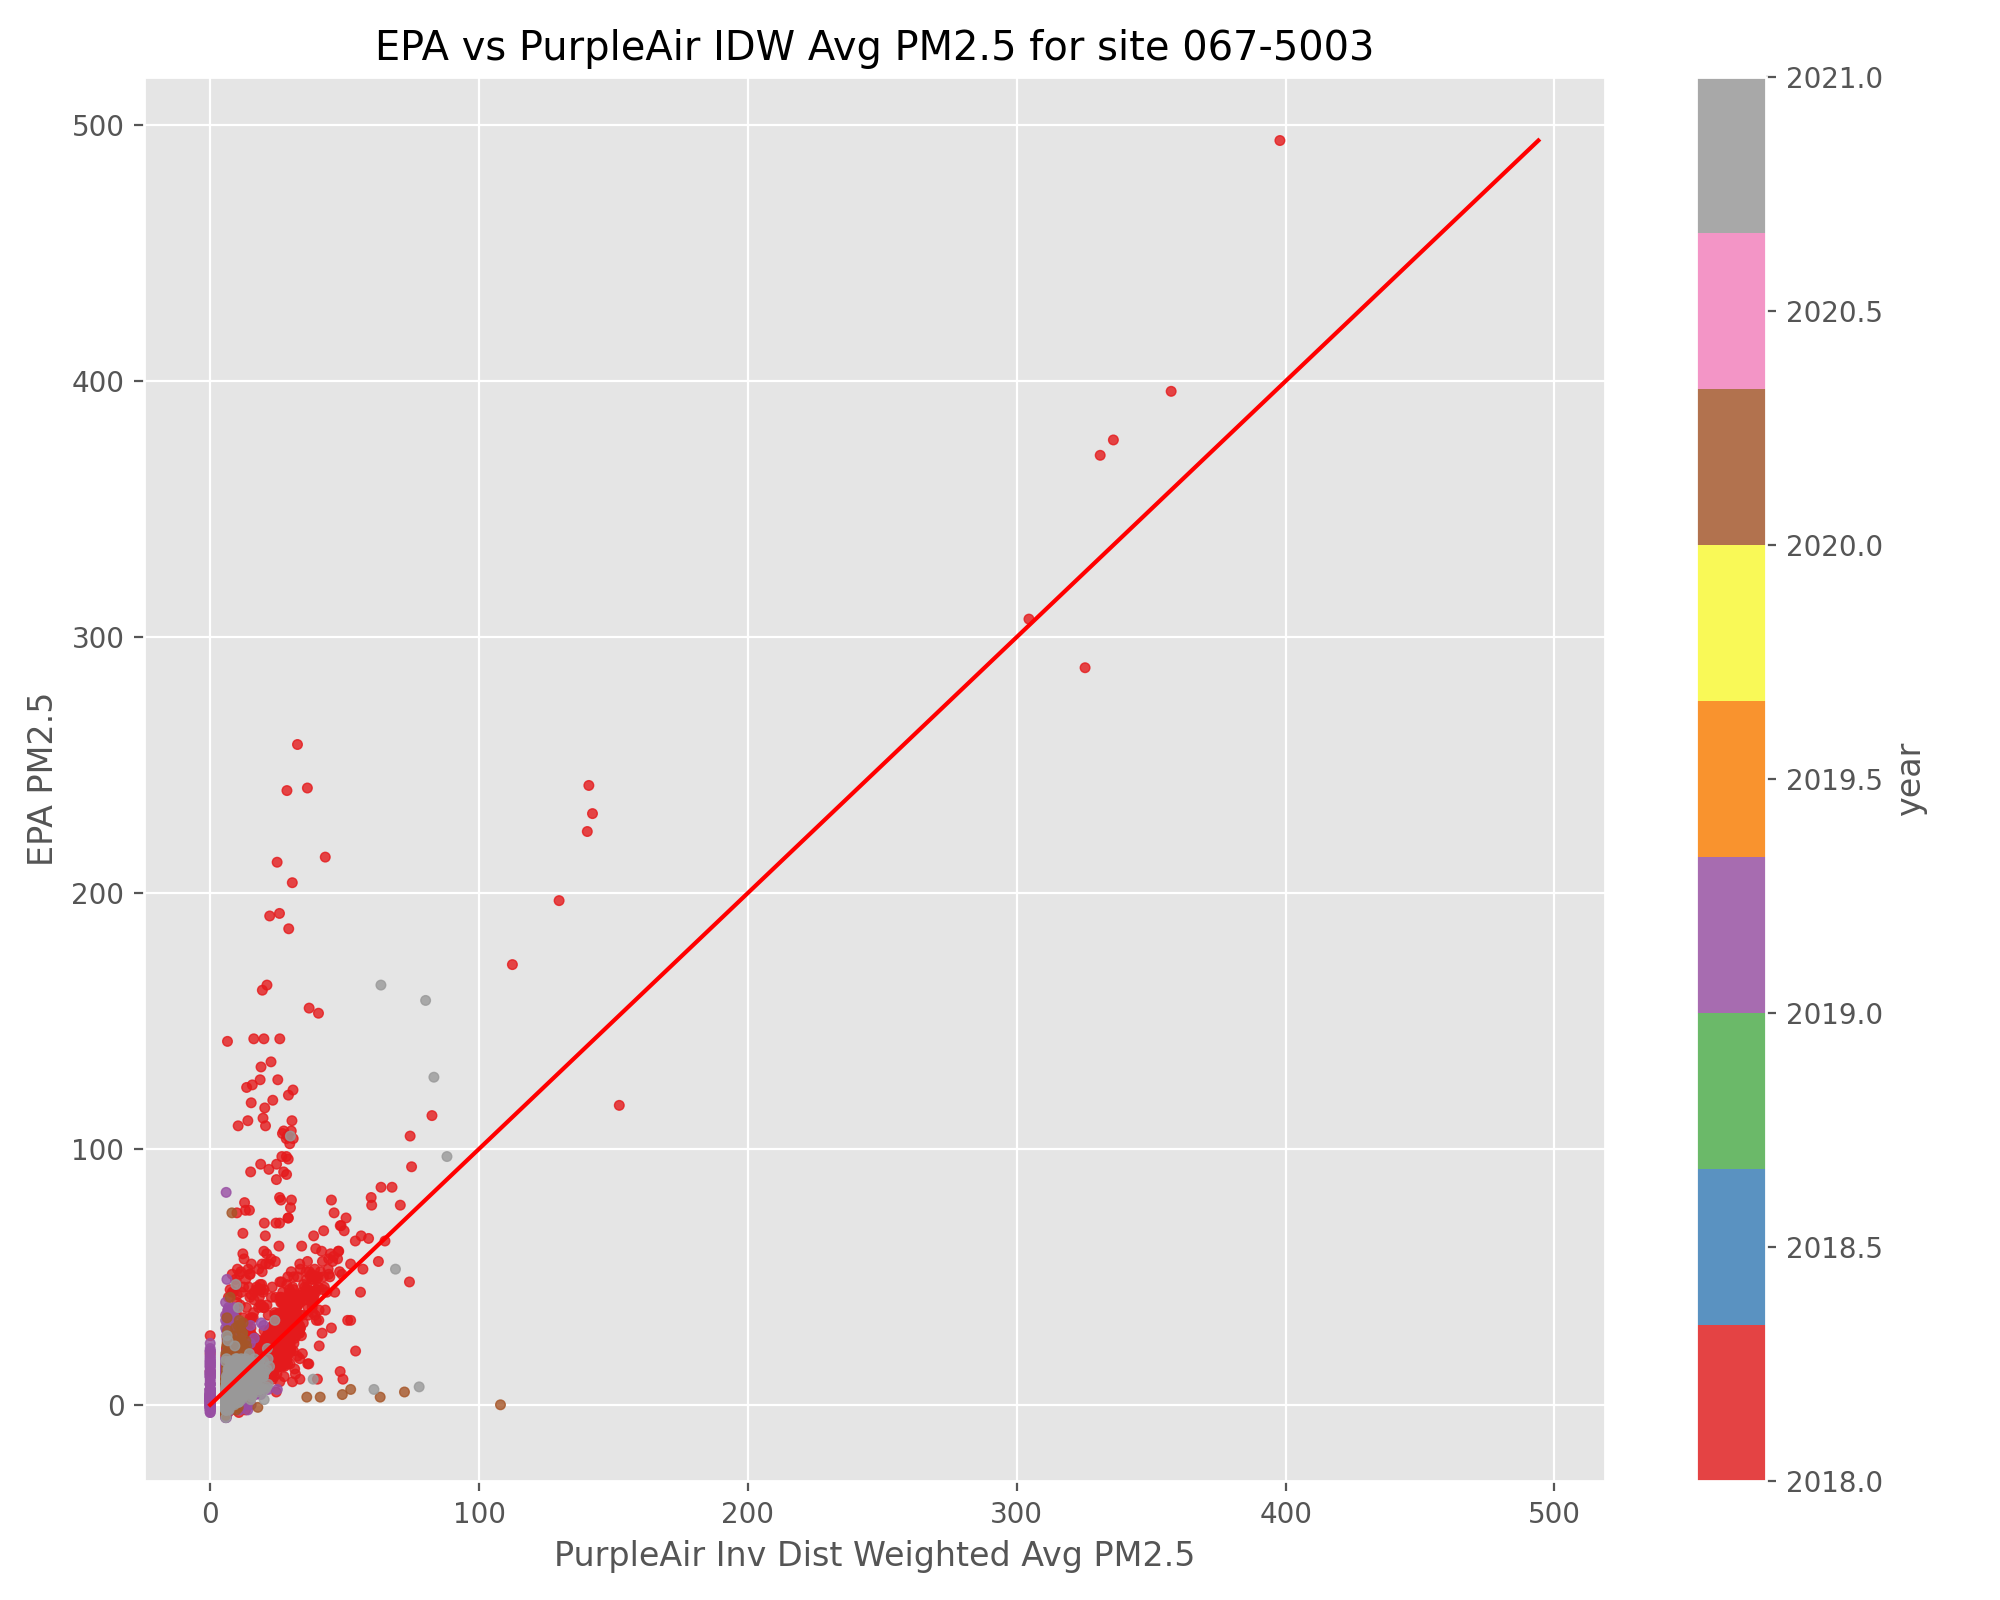
\includegraphics[width=0.8\textwidth]{appendix/site_plots/site-067-5003_epa-pa-hourly-plot.png}
\caption{Scatter plot comparing reported hourly PM2.5 measurements: the x-axis represents the IDW-weighted average of PurpleAir measurements, the y-axis represents reported NAAQS-primary monitor measurements. The red line is a 45$^\circ$ line, representing perfect correlation between the PurpleAir average and the NAAQS-primary monitor. This monitor is at site 5003 in county 067 (FIPS code).}
\label{fig:pa-epa-compare_067-5003}
\end{figure}
\begin{figure}
\centering
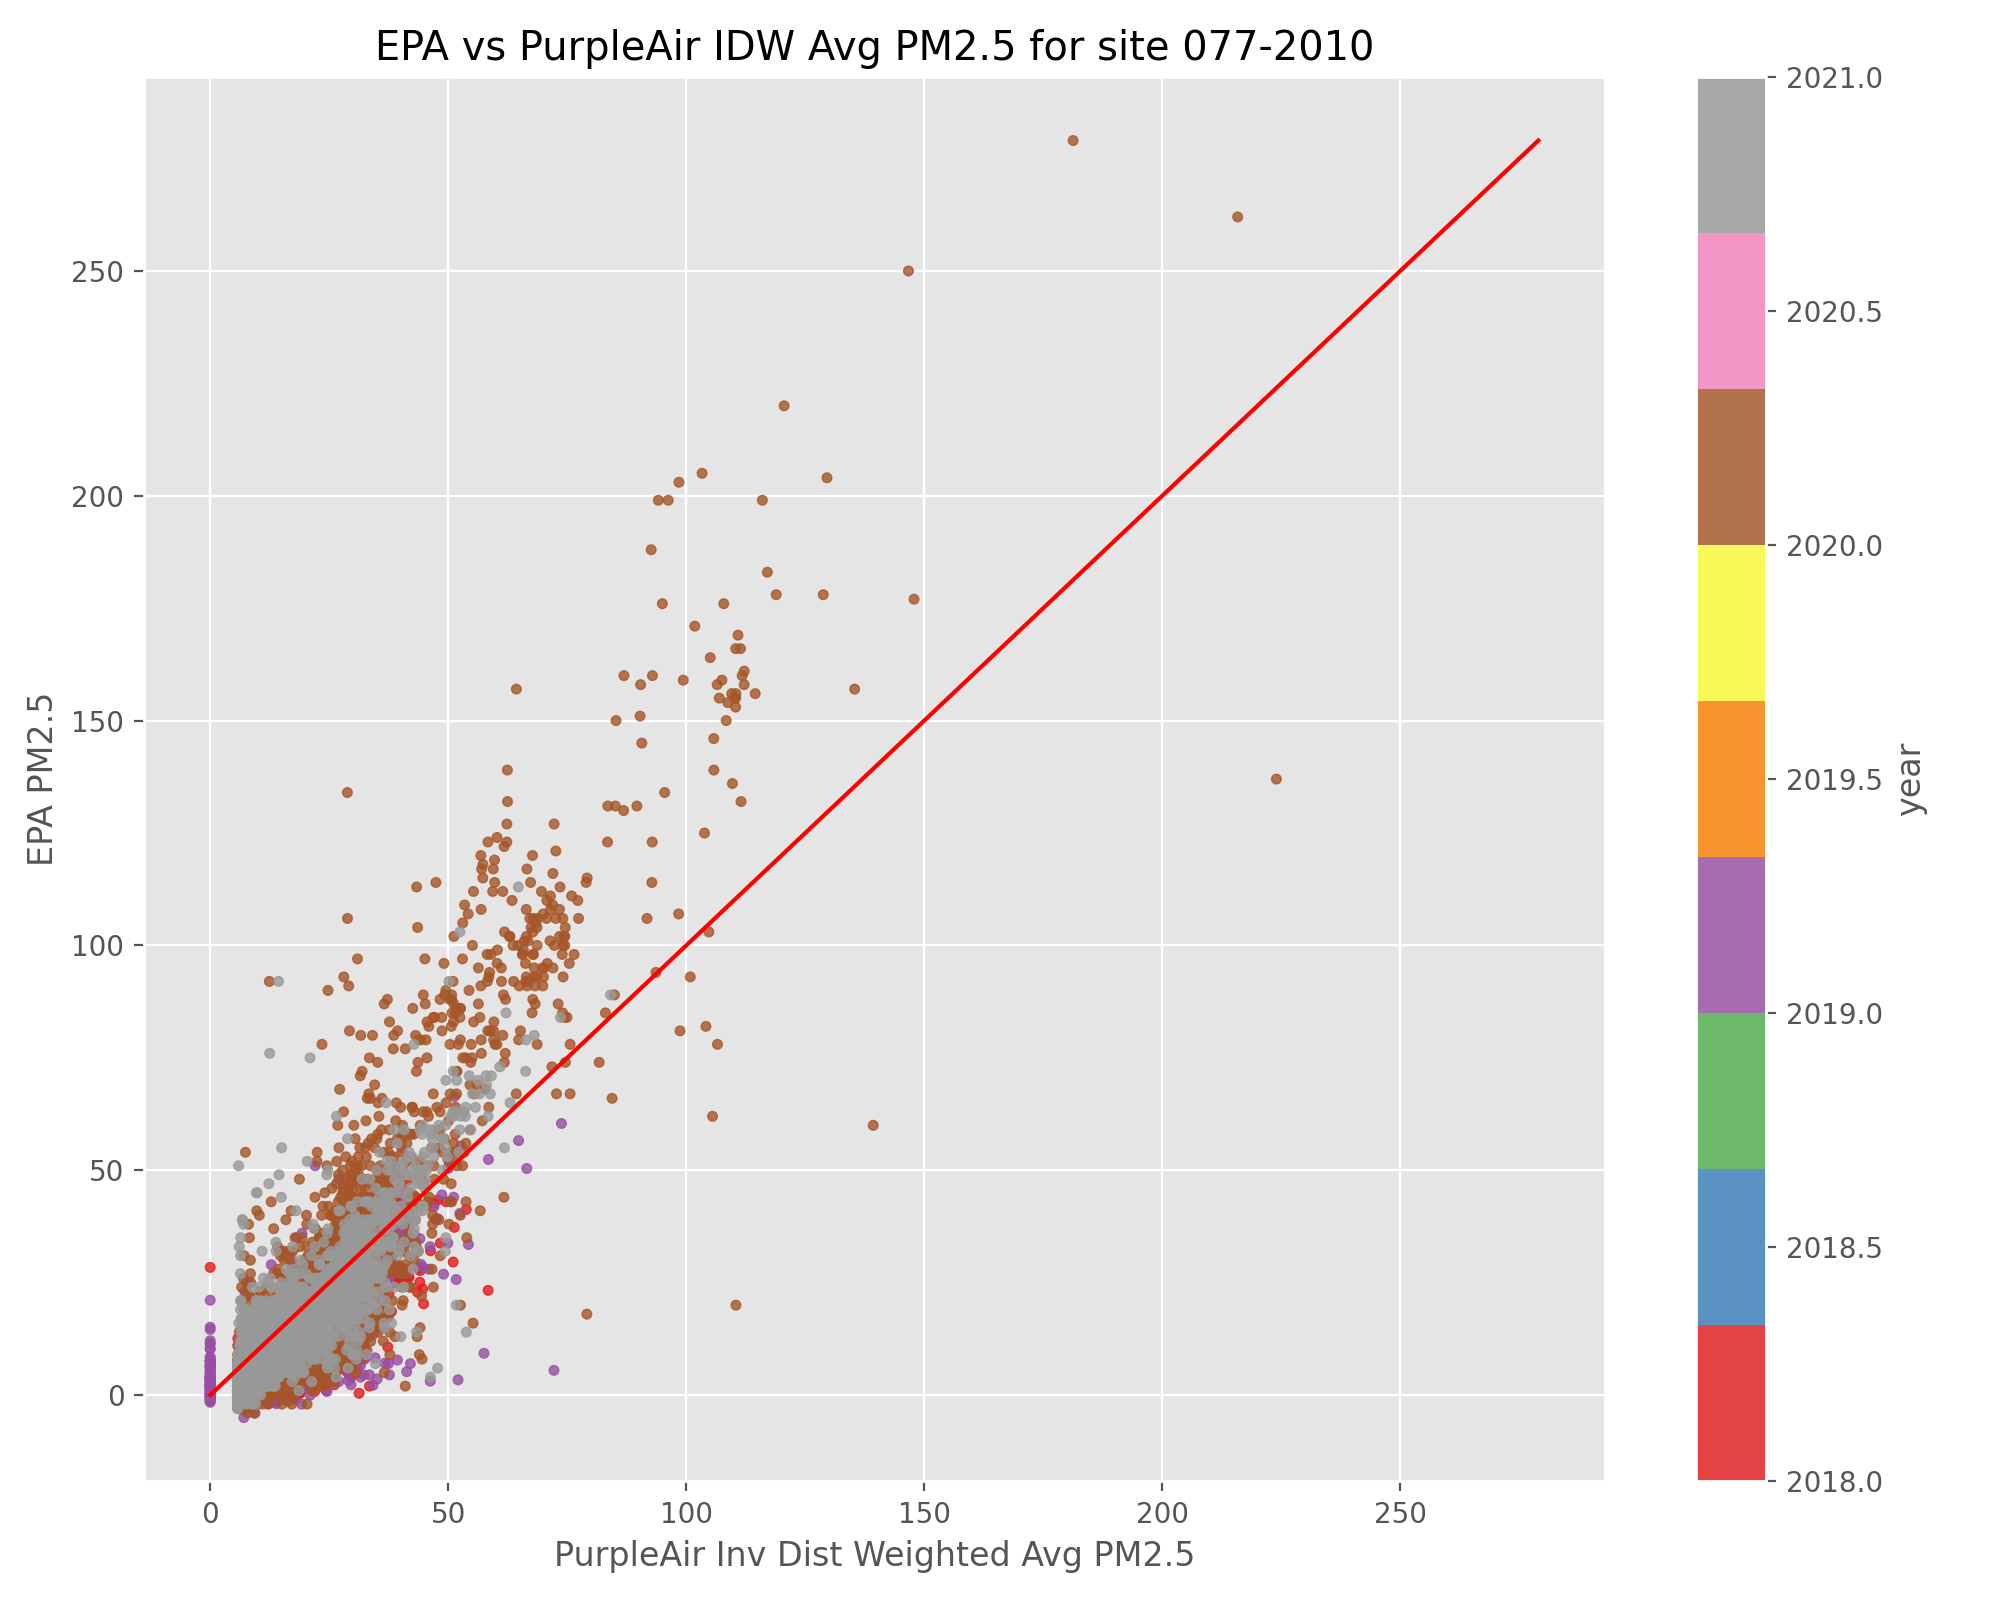
\includegraphics[width=0.8\textwidth]{appendix/site_plots/site-077-2010_epa-pa-hourly-plot.png}
\caption{Scatter plot comparing reported hourly PM2.5 measurements: the x-axis represents the IDW-weighted average of PurpleAir measurements, the y-axis represents reported NAAQS-primary monitor measurements. The red line is a 45$^\circ$ line, representing perfect correlation between the PurpleAir average and the NAAQS-primary monitor. This monitor is at site 2010 in county 077 (FIPS code).}
\label{fig:pa-epa-compare_077-2010}
\end{figure}
\begin{figure}
\centering
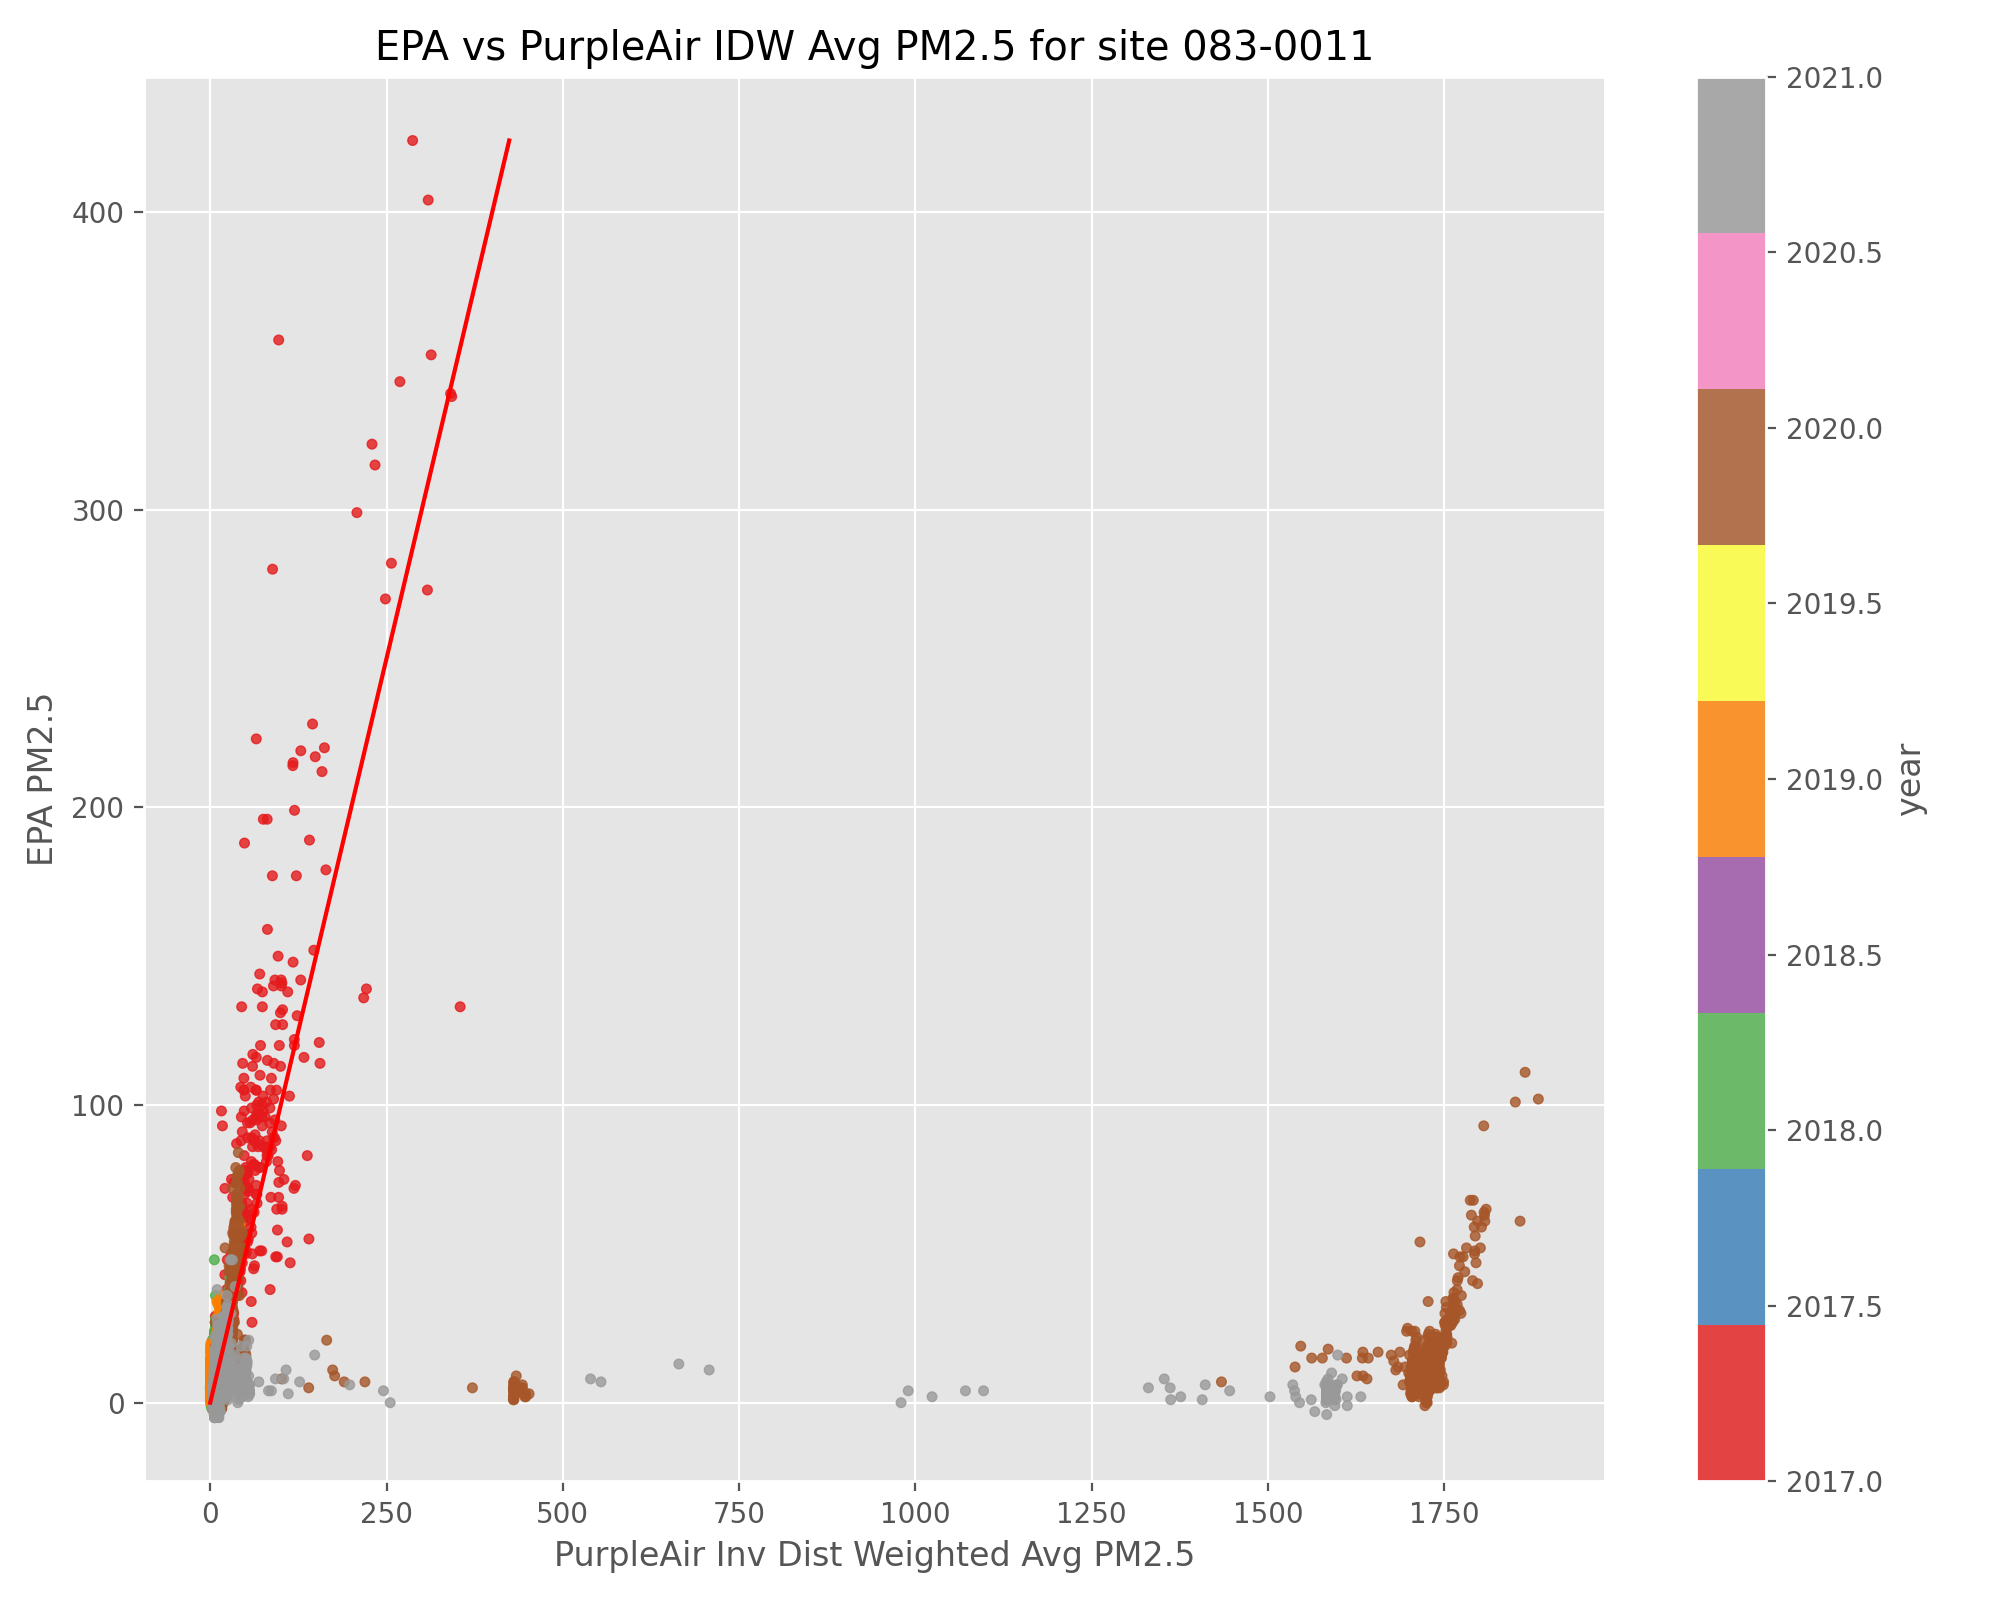
\includegraphics[width=0.8\textwidth]{appendix/site_plots/site-083-0011_epa-pa-hourly-plot.png}
\caption{Scatter plot comparing reported hourly PM2.5 measurements: the x-axis represents the IDW-weighted average of PurpleAir measurements, the y-axis represents reported NAAQS-primary monitor measurements. The red line is a 45$^\circ$ line, representing perfect correlation between the PurpleAir average and the NAAQS-primary monitor. This monitor is at site 0011 in county 083 (FIPS code).}
\label{fig:pa-epa-compare_083-0011}
\end{figure}
\begin{figure}
\centering
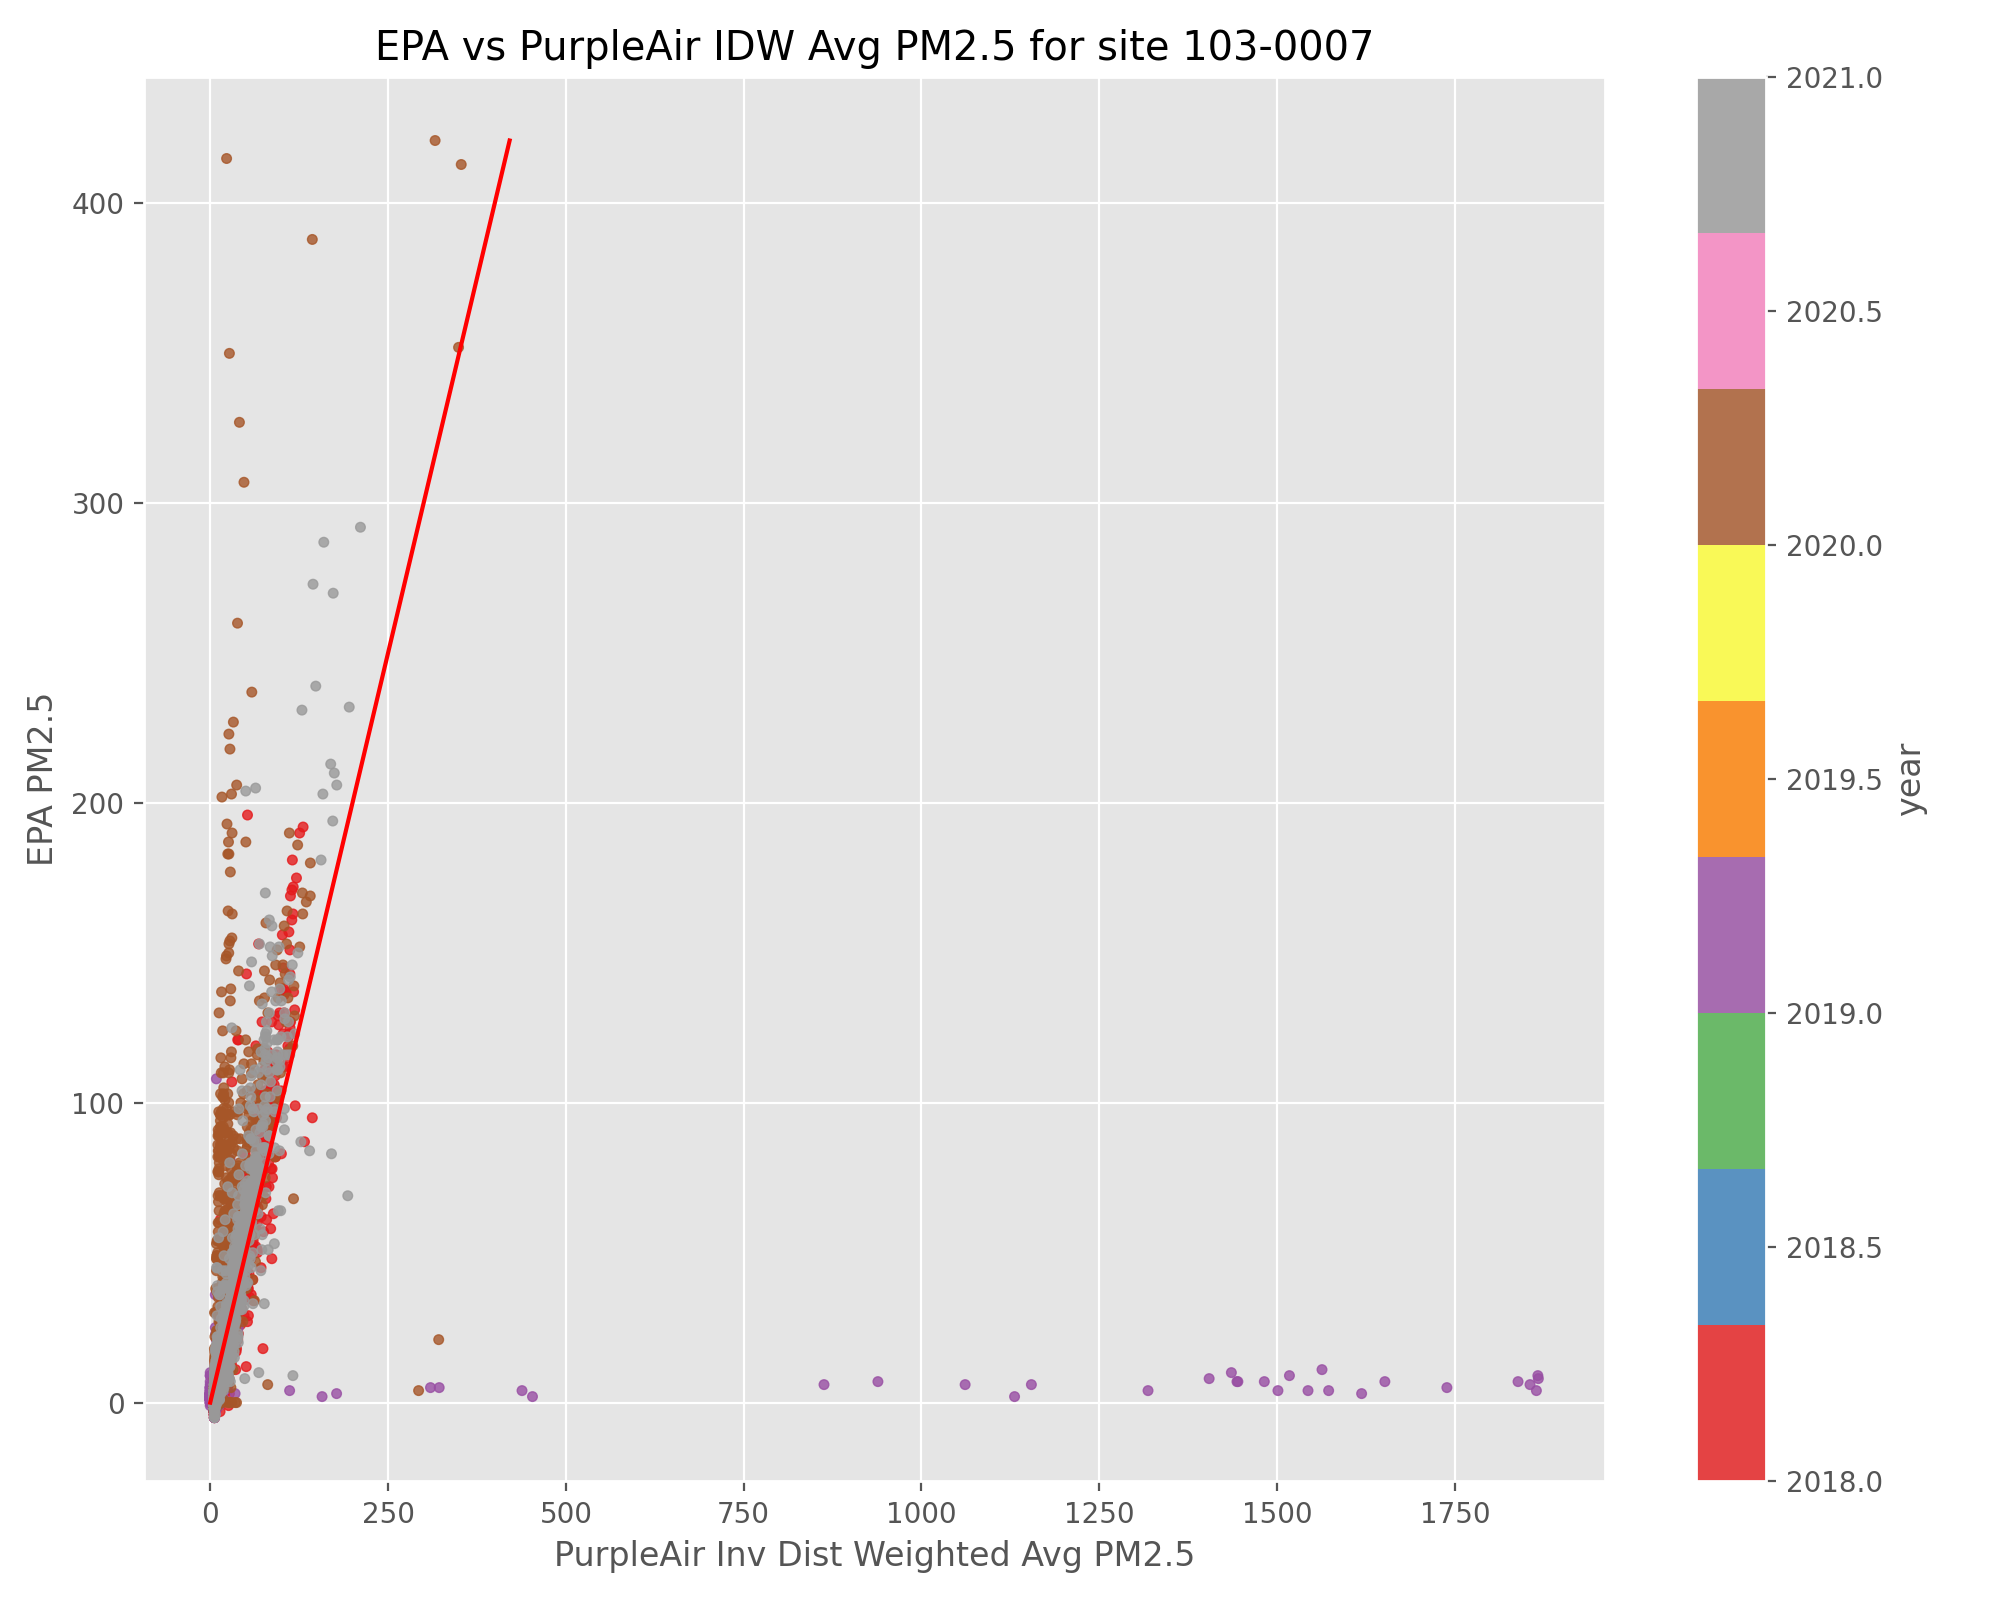
\includegraphics[width=0.8\textwidth]{appendix/site_plots/site-103-0007_epa-pa-hourly-plot.png}
\caption{Scatter plot comparing reported hourly PM2.5 measurements: the x-axis represents the IDW-weighted average of PurpleAir measurements, the y-axis represents reported NAAQS-primary monitor measurements. The red line is a 45$^\circ$ line, representing perfect correlation between the PurpleAir average and the NAAQS-primary monitor. This monitor is at site 0007 in county 103 (FIPS code).}
\label{fig:pa-epa-compare_103-0007}
\end{figure}
%=========================================
%  Kernel Density Comparison
%=========================================
\begin{figure}
\centering
\includegraphics[width=0.8\textwidth]{appendix/site_plots/site-001-0013_epa-pa-missing-density.png}
\caption{Comparison of PM2.5 concentration densities for two sets of hours: reported (blue) and missing (red) hourly observations of the NAAQS monitor. Both densities use the hourly PurpleAir PM2.5 concentration estimates for this site, calculated using the IDW average of PurpleAir sensors within 5 miles of the NAAQS monitor location. This monitor is at site 0013 in county 001 (FIPS code).}
\label{fig:missing-density_001-0013}
\end{figure}






\begin{figure}
\centering
\includegraphics[width=0.8\textwidth]{appendix/site_plots/site-019-5001_epa-pa-missing-density.png}
\caption{Comparison of PM2.5 concentration densities for two sets of hours: reported (blue) and missing (red) hourly observations of the NAAQS monitor. Both densities use the hourly PurpleAir PM2.5 concentration estimates for this site, calculated using the IDW average of PurpleAir sensors within 5 miles of the NAAQS monitor location. This monitor is at site 5001 in county 019 (FIPS code).}
\label{fig:missing-density_019-5001}
\end{figure}

\begin{figure}
\centering
\includegraphics[width=0.8\textwidth]{appendix/site_plots/site-027-0002_epa-pa-missing-density.png}
\caption{Comparison of PM2.5 concentration densities for two sets of hours: reported (blue) and missing (red) hourly observations of the NAAQS monitor. Both densities use the hourly PurpleAir PM2.5 concentration estimates for this site, calculated using the IDW average of PurpleAir sensors within 5 miles of the NAAQS monitor location. This monitor is at site 0002 in county 027 (FIPS code).}
\label{fig:missing-density_027-0002}
\end{figure}

\begin{figure}
\centering
\includegraphics[width=0.8\textwidth]{appendix/site_plots/site-029-0018_epa-pa-missing-density.png}
\caption{Comparison of PM2.5 concentration densities for two sets of hours: reported (blue) and missing (red) hourly observations of the NAAQS monitor. Both densities use the hourly PurpleAir PM2.5 concentration estimates for this site, calculated using the IDW average of PurpleAir sensors within 5 miles of the NAAQS monitor location. This monitor is at site 0018 in county 029 (FIPS code).}
\label{fig:missing-density_029-0018}
\end{figure}

\begin{figure}
\centering
\includegraphics[width=0.8\textwidth]{appendix/site_plots/site-039-2010_epa-pa-missing-density.png}
\caption{Comparison of PM2.5 concentration densities for two sets of hours: reported (blue) and missing (red) hourly observations of the NAAQS monitor. Both densities use the hourly PurpleAir PM2.5 concentration estimates for this site, calculated using the IDW average of PurpleAir sensors within 5 miles of the NAAQS monitor location. This monitor is at site 2010 in county 039 (FIPS code).}
\label{fig:missing-density_039-2010}
\end{figure}

\begin{figure}
\centering
\includegraphics[width=0.8\textwidth]{appendix/site_plots/site-057-0005_epa-pa-missing-density.png}
\caption{Comparison of PM2.5 concentration densities for two sets of hours: reported (blue) and missing (red) hourly observations of the NAAQS monitor. Both densities use the hourly PurpleAir PM2.5 concentration estimates for this site, calculated using the IDW average of PurpleAir sensors within 5 miles of the NAAQS monitor location. This monitor is at site 0005 in county 057 (FIPS code).}
\label{fig:missing-density_057-0005}
\end{figure}

\begin{figure}
\centering
\includegraphics[width=0.8\textwidth]{appendix/site_plots/site-059-0007_epa-pa-missing-density.png}
\caption{Comparison of PM2.5 concentration densities for two sets of hours: reported (blue) and missing (red) hourly observations of the NAAQS monitor. Both densities use the hourly PurpleAir PM2.5 concentration estimates for this site, calculated using the IDW average of PurpleAir sensors within 5 miles of the NAAQS monitor location. This monitor is at site 0007 in county 059 (FIPS code).}
\label{fig:missing-density_059-0007}
\end{figure}

\begin{figure}
\centering
\includegraphics[width=0.8\textwidth]{appendix/site_plots/site-067-5003_epa-pa-missing-density.png}
\caption{Comparison of PM2.5 concentration densities for two sets of hours: reported (blue) and missing (red) hourly observations of the NAAQS monitor. Both densities use the hourly PurpleAir PM2.5 concentration estimates for this site, calculated using the IDW average of PurpleAir sensors within 5 miles of the NAAQS monitor location. This monitor is at site 5003 in county 067 (FIPS code).}
\label{fig:missing-density_067-5003}
\end{figure}

\begin{figure}
\centering
\includegraphics[width=0.8\textwidth]{appendix/site_plots/site-077-2010_epa-pa-missing-density.png}
\caption{Comparison of PM2.5 concentration densities for two sets of hours: reported (blue) and missing (red) hourly observations of the NAAQS monitor. Both densities use the hourly PurpleAir PM2.5 concentration estimates for this site, calculated using the IDW average of PurpleAir sensors within 5 miles of the NAAQS monitor location. This monitor is at site 2010 in county 077 (FIPS code).}
\label{fig:missing-density_077-2010}
\end{figure}

\begin{figure}
\centering
\includegraphics[width=0.8\textwidth]{appendix/site_plots/site-083-0011_epa-pa-missing-density.png}
\caption{Comparison of PM2.5 concentration densities for two sets of hours: reported (blue) and missing (red) hourly observations of the NAAQS monitor. Both densities use the hourly PurpleAir PM2.5 concentration estimates for this site, calculated using the IDW average of PurpleAir sensors within 5 miles of the NAAQS monitor location. This monitor is at site 0011 in county 083 (FIPS code).}
\label{fig:missing-density_083-0011}
\end{figure}

\begin{figure}
\centering
\includegraphics[width=0.8\textwidth]{appendix/site_plots/site-103-0007_epa-pa-missing-density.png}
\caption{Comparison of PM2.5 concentration densities for two sets of hours: reported (blue) and missing (red) hourly observations of the NAAQS monitor. Both densities use the hourly PurpleAir PM2.5 concentration estimates for this site, calculated using the IDW average of PurpleAir sensors within 5 miles of the NAAQS monitor location. This monitor is at site 0007 in county 103 (FIPS code).}
\label{fig:missing-density_103-0007}
\end{figure}


\end{document}
